\documentclass[12pt,a4paper,openright,twoside]{book}
\usepackage[utf8]{inputenc}
\usepackage{phd-thesis}
\usepackage{code-lstlistings}
\usepackage{notes}
\usepackage{shortcuts}
\usepackage{svg}
\usepackage{booktabs}
\usepackage{tabularx}
\usepackage{array}
\usepackage{amssymb}
\usepackage[table]{xcolor}
\usepackage{xspace}
\usepackage{pifont}

\newcommand{\prop}[2]{(\texttt{#1},\;#2)\xspace}
\newcommand{\lbl}[1]{\texttt{#1}\xspace}
\newcommand{\ftemporal}{\tau}
\newcommand{\fts}{\phi}
\newcommand{\oot}{\textit{OoT}}
\newcommand{\ourapproach}{STGraph\xspace}
\newcommand{\eop}{\hfill $\Box$}  
\renewcommand{\sf}[1]{\textsf{\textup{#1}}}  
\renewcommand{\tt}[1]{\texttt{\textup{#1}}}  


\newcommand{\algemph}[1]{\algcolor{lightgray}{#1}}
\renewcommand{\sf}[1]{\textsf{\textup{#1}}}
\newcommand{\answer}[1]{\answerns{#1}\\}
\newcommand{\answerns}[1]{$\Box$ #1}
\newcommand{\dfd}[1]{\textup{#1}}
\newcommand{\serv}[1]{\tt{#1}}

% --- pacchetti (se non già presenti nel preambolo della tesi) ---
\usepackage{algorithm}
\usepackage{algpseudocode}
\algdef{SE}[SWITCH]{Switch}{EndSwitch}[1]{\textbf{switch} #1}{\textbf{end switch}}
\algdef{SE}[CASE]{Case}{EndCase}[1]{\textbf{case} #1}{}
\algtext*{EndCase}
\algnewcommand\algorithmicforeach{\textbf{for each}}
\algdef{S}[FOR]{ForEach}[1]{\algorithmicforeach\ #1\ \algorithmicdo}
\algdef{SE}[DOWHILE]{Do}{doWhile}{\algorithmicdo}[1]{\algorithmicwhile\ #1}%
\newcommand{\algcolor}[2]{\hspace*{-\fboxsep}\colorbox{#1}{\parbox{\linewidth}{#2}}}
\usepackage{listings}
\usepackage{booktabs}
\usepackage{multirow}
\usepackage{subcaption}
\usepackage{threeparttable}


% --- ambienti numerati (se non già definiti altrove nella tesi) ---
\newtheorem{definition}{Definition}[chapter]
\newtheorem{example}{Example}[chapter]

% --- stile per il listato Cypher ---
\lstdefinestyle{mystyle}{
    commentstyle=\color{gray},
    keywordstyle=\color{magenta},
    basicstyle=\ttfamily\footnotesize,
    keywords={MATCH,WHERE,RETURN},
    breaklines=true,
    keepspaces=true,
    showstringspaces=false,
}
\lstset{style=mystyle}
% Definizione di una colonna X allineata a sinistra
\newcolumntype{Y}{>{\raggedright\arraybackslash}X}


\definecolor{mpgreen}{RGB}{76, 153, 0}
\newcommand{\mpa}[1]{{\color{mpgreen}#1}}

\mainlinespacing{1.241} % line spacing in mainmatter, comment to default (1)

\begin{document}
	
\frontmatter
\input{front}

\begin{abstract}
Max 2000 characters, strict.
\end{abstract}

\begin{dedication} % this is optional
Dedication
\end{dedication}

\begin{acknowledgements} % this is optional
Pippo
\end{acknowledgements}

%----------------------------------------------------------------------------------------
\tableofcontents   
\listoffigures     % (optional) comment if empty
\lstlistoflistings % (optional) comment if empty
%----------------------------------------------------------------------------------------

\mainmatter

%----------------------------------------------------------------------------------------
\begin{introduction}
\label{chap:introduction}
\section*{Context and Motivations}
\addcontentsline{toc}{section}{Context and Motivations}

Throughout the course of its evolution, human society has been continuously and profoundly shaped by the advancement of technology.
%
From the invention of the wheel to the advent of personal computers, each technological breakthrough has had profound effects on how individuals interact with one another and with their environment.
%
Since the turn of the millennium, the rise of digital technologies has transformed the way we live, work, and communicate, propelling humankind into a new digital era.
%
As society transitioned toward this digital paradigm, the concept of data began to gain value, ultimately becoming pivotal in what is now referred to as a digital society.
%
As this digital transformation continues to unfold, driven by the widespread adoption of cloud infrastructures, smart services, and the Internet of Things (IoT), generated data has exponentially grown \mpa{{some\_ref}} not only in sheer volume but also in variety, presenting unprecedented opportunities alongside critical challenges in data management.
%
Furthermore, the availability of vast amounts of data has paved the way for the practical deployment of advanced, data-intensive technologies, such as machine learning, artificial intelligence, and digital twins.
%
Despite their long-standing theoretical foundations, these approaches remained constrained for decades by a lack of adequate computational infrastructure and sufficient data, but are now actively transforming numerous aspects of society.

Within the past decade, the emergence of digital twins has garnered significant attention across multiple domains, including manufacturing, healthcare, smart cities, and agriculture.
%
A digital twin represents one of the most advanced paradigms enabled by digital transformation, serving as a dynamic virtual replica of a physical entity, a complex system, or operational process.
%
By capturing the physical entity's underlying characteristics and continuously reflecting its state and behavior, a digital twin enables advanced simulation, predictive modeling, monitoring, and performance optimization within a virtual environment.

As reflected by their progression along the Gartner Hype Cycle~\mpa{{some\_ref}}, digital twins have evolved from an emerging research concept into an increasingly adopted technological paradigm across a wide range of application domains.
%
However, this growing maturity has also exposed significant limitations that hinder their large-scale adoption and, in particular, the development of interoperable Digital Twin.
%
Most existing digital twins have been developed as domain-specific, vertically integrated solutions, independently designed to address the requirements of individual application scenarios.
%
As a result, they rely on heterogeneous software architectures, data representations, and application-specific information models, leading to fragmented data environments in which the information generated by individual digital twins remains largely confined within isolated silos.
%
This fragmentation hinders the integration and reuse of data across independently developed digital twins, ultimately limiting interoperability, scalability, and the applicability of digital twin ecosystems to more complex, cross-domain scenarios.

Achieving interoperability is therefore becoming a fundamental requirement for the next generation of digital twin systems and, consequently, for the software infrastructures supporting them.
%
Beyond enabling information exchange, interoperability provides the foundation for integrating independently developed digital twins into larger ecosystems, where heterogeneous information can be jointly analyzed and exploited to support increasingly complex cyber-physical scenarios.
%
This challenge can be considered from two complementary dimensions.
%
The first concerns the software infrastructure supporting digital twins. Current implementations are typically developed as self-contained solutions, creating the need for common architectural foundations capable of supporting the deployment, integration, and management of heterogeneous digital twins within shared environments.
%
The second concerns the data management and semantic dimension. Even when digital twins can be deployed within a common infrastructure, the heterogeneity of the data they produce and consume, together with the use of domain-specific data models, schemas, and representations, poses significant challenges to data integration.
%
Data originating from different digital twins may differ not only in their structure and format, but also in their temporal characteristics, granularity, metadata, and underlying semantics, making their integration and joint querying a non-trivial data management problem.
%
Addressing these challenges requires common approaches to data modeling, integration, and governance, together with architectural foundations capable of supporting the heterogeneous and continuously evolving workloads associated with digital twin applications.
%
Taken together, these requirements motivate the development of software infrastructures specifically designed to support digital twin ecosystems rather than individual digital twins in isolation.

These requirements point toward the need for dedicated software infrastructures capable of supporting the deployment, management, and integration of heterogeneous digital twins within a shared environment.
%
Such infrastructures can be envisioned as Digital Twin Platforms (DTPs): software environments designed around the specific data and operational requirements of digital twin systems, providing the architectural and data management foundations required to deploy, integrate, and manage multiple digital twins within a common environment.
%
A Digital Twin Platform therefore provides a natural architectural foundation for addressing the fragmentation of current digital twin solutions, bringing together the infrastructure and data management mechanisms required to support digital twin ecosystems.
%
The importance of such foundations is likely to become even more pronounced with the recent emergence of large language models and increasingly capable agentic systems.
%
By combining access to heterogeneous information with advanced reasoning and decision-making capabilities, these technologies may enable digital twins to evolve from primarily reactive representations of physical systems toward more proactive entities capable of autonomously analyzing information, initiating actions, and, ultimately, interacting with other digital twins.
%
Emerging visions of interconnected digital twins forming distributed ``Digital Brains'' further illustrate the potential of this evolution.
%
However, realizing such scenarios requires digital twins to first overcome their current fragmentation: the ability of intelligent agents to reason over information, communicate, and coordinate actions ultimately depends on interoperable underlying systems and shared representations of the data they exchange.
%
In this context, Digital Twin Platforms can provide the common technological foundation upon which such interconnected ecosystems can be built, combining architectural support for heterogeneous digital twins with the data management capabilities required to make their information accessible, interpretable, and interoperable.

\section*{Overview and Contribution}
\addcontentsline{toc}{section}{Overview and Contribution}

This thesis approaches these challenges from a data-oriented perspective, arguing that the development of interoperable Digital Twin ecosystems should be grounded in the data they collect, produce, and exchange.
%
Rather than considering the digital twin primarily as a standalone software application, the work first investigates the characteristics and requirements of the underlying data produced and exploited by digital twins, using them as the basis for identifying suitable data models and mechanisms for their integration and management.
%
From this perspective, establishing common data models and, where possible, standardized representations for digital twins constitutes a fundamental step toward interoperability and, consequently, toward the design of effective Digital Twin Platforms.
%
Once these data requirements and representations have been established, the corresponding software infrastructure can be designed according to the characteristics of the data and the operational requirements of digital twin systems.
%
This includes supporting heterogeneous data sources, different data models and formats, varying collection frequencies, and continuous data streams, while providing the scalability and architectural capabilities required by distributed digital twin deployments.
%
The thesis therefore follows a bottom-up perspective, moving from data characteristics and requirements, through data modeling and management, toward the architectural foundations required to support interoperable Digital Twin ecosystems.
%
Within this perspective, the Digital Twin Platform represents the architectural context in which these elements are brought together: a common software foundation in which digital twins can be deployed and managed, while their heterogeneous data can be integrated, governed, and exploited across the ecosystem.
%
Such infrastructures can be envisioned as a Digital Twin Platform:
in this thesis, such term is used to denote a standardized framework that supports the modeling, deployment, management, and interoperability of ecosystems of Digital Twins throughout their lifecycle.
%
Rather than treating data management as a supporting component of the platform, this perspective places data at the core of its design, providing a foundation for addressing the architectural requirements of interoperable digital twin ecosystems.
%
Accordingly, the thesis investigates the Digital Twin Platform not merely as an infrastructure for hosting digital twins, but as a software and data management foundation through which heterogeneous digital twins can be integrated into interoperable ecosystems.

\subsection*{Problem Statement}

The goal of this thesis is to contribute to the development of interoperable Digital Twin ecosystems through the investigation of architectures and methods for Digital Twin Platforms, adopting a data-oriented perspective.
The research focuses on understanding the data management challenges arising from Digital Twin applications and on identifying the models, technologies, methods, and architectural foundations required to address them within a common platform.
%
Working towards this goal, the thesis investigates the following research questions:

\begin{rqlist}
\item[RQ1] \textit{What are the data characteristics and requirements emerging from Digital Twin applications, and to what extent can existing data management technologies satisfy them?}

\item[RQ2] \textit{How can data models, data management approaches, and governance mechanisms support the integration and interoperability of heterogeneous Digital Twin data?} 

\item[RQ3] \textit{How can software architectures support the deployment and management of heterogeneous Digital Twins while satisfying their data and operational requirements?} 

\end{rqlist}


Together, these questions follow the bottom-up perspective adopted throughout the thesis, moving from the characteristics and requirements of Digital Twin data toward the data models, management mechanisms, governance approaches, and software architectures required to support interoperable Digital Twin ecosystems. The answers to these questions contribute to the definition of the architectural and methodological foundations of a Digital Twin Platform, conceived as a common environment for the deployment, management, integration, and interoperability of ecosystems of Digital Twins.

\subsection*{Contributions}
\mpa{list of publications with brief description}

\subsection*{Structure of the thesis}
Accordingly, the thesis is organized into three main parts, each addressing a different aspect of the research problem and contributing to the development of the Digital Twin Platform from complementary perspectives.

\paragraph{Foundations}
\Cref{part:foundations} provides the background notions and concepts required to understand the context and research problem addressed in this thesis.
%
In \Cref{chap:evolving_intertwined_world}, a background is provided on the growing value of data in the digital society, illustrating how the increasing availability of large-scale data has enabled the adoption of advanced data-intensive technologies, including digital twins, and how data management solutions are evolving to meet these demands.
%
In \Cref{chap:digital_twins} the thesis provides a background on digital twins, illustrating their evolution from a research concept to an adopted technological paradigm, and highlighting the challenges that currently hinder their large-scale adoption.
%
Finally, in \Cref{chap:data_oriented_perspective} and within the broader vision of a Digital Twin Platform, the thesis identifies the main characteristics and requirements of digital twin data, illustrating how they can be used to inform the design of data models, management mechanisms, and software infrastructures capable of supporting interoperable digital twin ecosystems.

\paragraph{Architectures}
In \Cref{part:architectures}, the thesis investigates the architectural foundations required to support interoperable digital twin ecosystems within a Digital Twin Platform.
%
Specifically, in \Cref{chap:dataplat} and within a national research project, the thesis explores a data platform solution tailored for precision agriculture, identifying and illustrating the requirements of digital twin applications and how they can be addressed through a general-purpose software infrastructure.
%
This work provides a concrete architectural perspective on how the data and operational requirements identified in the foundations of the thesis can be translated into platform capabilities.
%
Complementarily, following the requirements identified in \Cref{chap:dataplat}, \Cref{chap:stgraph} presents a data model for digital twins, illustrating how such requirements can be addressed through a dedicated and novel data management approach within a Digital Twin Platform.

\paragraph{Methods and applications}
In \Cref{part:methods-applications} and based on the previous findings, the thesis investigates governance techniques and methods facilitating the management of digital twin data within a Digital Twin Platform.
%
In \Cref{sec:process-driven-design}, a methodology is proposed to guide the deployment of data-intensive applications within a data platform, illustrating how the characteristics of the data can be used to produce a blueprint for the design of the underlying software infrastructure.
%
Similarly, in \Cref{sec:llm-guided-metadata-exploration}, a method is proposed to facilitate the governance of heterogeneous data, leveraging large language models to support the discovery and understanding of their metadata.
%
These methods complement the architectural and data management foundations of the Digital Twin Platform by addressing the processes required to design, deploy, and govern data-intensive applications within it.

Finally, in \Cref{chap:applications}, the thesis illustrates some applications relying on the proposed Digital Twin Platform.
%
Within \Cref{sec:smarter}, the thesis presents a digital twin application for precision agriculture and illustrates how the proposed platform can be used to support its deployment and operation.
%
In \Cref{sec:s2g}, the thesis presents a novel technique for anomaly detection in complex sensor networks, illustrating how, within a Digital Twin Platform, the previously identified data model and management techniques can enable novel data analytics.

\end{introduction}
%----------------------------------------------------------------------------------------

%

%%%%%%%%%%%%%%%%%%%%%%%%%%%
%%%%%%%%%%%%%%%%%%%%%%%%%%%

\part{Foundations}
\label{part:foundations}
%%%%%%%%%%%%%%%%%%%%%%%%%%%
\chapter{An Evolving and Intertwined World}
\label{chap:evolving_intertwined_world}
The ongoing digital transformation of science, industry, and society has progressively changed both the role assigned to data and the software infrastructures used to manage it. Early information systems were primarily concerned with recording and managing operational events. As analytical techniques and computational infrastructures matured, these records became the basis for information, knowledge, and decision support. Subsequently, the widespread deployment of sensors, connected devices, distributed computing, and streaming infrastructures extended the scope of digital systems from enterprise processes to continuously monitored physical environments.

This evolution can therefore be considered from two complementary and increasingly intertwined perspectives. The first concerns the changing role and value attributed to data: from a record of an event, to information about that event, to knowledge derived from collections of observations, and ultimately to a basis for decision and action. The second concerns the evolution of the computational infrastructures required to support these transformations: from transactional information systems and analytical warehouses to distributed cloud data platforms, continuous processing infrastructures, and cyber-physical systems.

The two trajectories are not independent. Each new class of systems has emerged in response to new requirements concerning the scale, variety, timeliness, and use of data, while the increasing availability of data has, in turn, enabled new computational capabilities. The history of digital systems can therefore be interpreted not simply as a succession of technologies, but as an intertwined evolution in which changes in the role of data and changes in computing infrastructures continuously influence one another.

These trajectories increasingly converge as digital systems become capable of continuously observing and interacting with physical processes. Data is no longer only a record of what has happened, but a basis for understanding what is happening, estimating what may happen next, and supporting decisions concerning what should happen. This progression provides the technological and conceptual background against which the recent proliferation of Digital Twin systems and artificial intelligence should be understood.

This chapter traces these developments as a foundation for the remainder of the thesis. It focuses on the evolution of data and of the computational infrastructures surrounding it, with particular attention to the changing requirements for data management that accompanied each stage.

% =========================================================================
\section{Digitalization -- From Data to Wisdom}
\label{sec:digitalization_data_knowledge}
% =========================================================================

The history of digital information systems can be interpreted as a progressive transformation in the role of data. In the earliest stages of electronic data processing, computational systems were primarily employed to automate repetitive calculations and to maintain records of organizational activities. Financial transactions, inventory movements, administrative records, and other operational events were represented as structured data whose primary purpose was to document the state of an organization and support the execution of its processes.

The introduction of the relational data model provided a rigorous foundation for the management of such information. Relational Database Management Systems, together with Online Transaction Processing (OLTP), established an architectural paradigm centered on structured schemas, transactional consistency, integrity constraints, and reliable updates \cite{codd1970,gray1992}. At this stage, the requirements imposed on data management were therefore primarily concerned with correctness, consistency, persistence, and efficient access to operational data. Data was mainly an operational asset: its value depended on its ability to faithfully represent the state of the processes that generated it.

As organizations accumulated increasing amounts of operational data, a new opportunity emerged. Data generated by individual transactions could also be exploited beyond the process in which it had originally been produced. Organizations began to integrate data across processes and over time in order to obtain aggregated indicators, identify historical patterns, compare operational states, and support planning and management decisions. This shift motivated the development of Data Warehousing and Business Intelligence architectures, which enabled integrated and multidimensional analysis of historical organizational data \cite{inmon1992,kimball2002}.

The role of data consequently expanded from operational record to analytical resource. Transactional systems were primarily concerned with faithfully recording the state of operational processes, whereas analytical infrastructures enabled organizations to examine trends, correlations, historical behaviour, and organizational performance across time and across processes. The change was not only a change in how data was used; it also introduced new requirements for how data had to be managed. Data originating from multiple operational systems had to be integrated, consolidated, transformed, and organized according to analytical purposes.

A useful conceptual representation of this progression is provided by the Data--Information--Knowledge--Wisdom (DIKW) framework (\Cref{fig:dikw}). Widely discussed as a conceptual model of increasing levels of meaning, it distinguishes between data as observations, information as contextualized and organized data, knowledge as the result of identifying relationships and patterns, and wisdom as the informed application of knowledge to judgement and decision making \cite{ackoff1989,rowley2007}.

\begin{figure}[htbp]
    \centering
    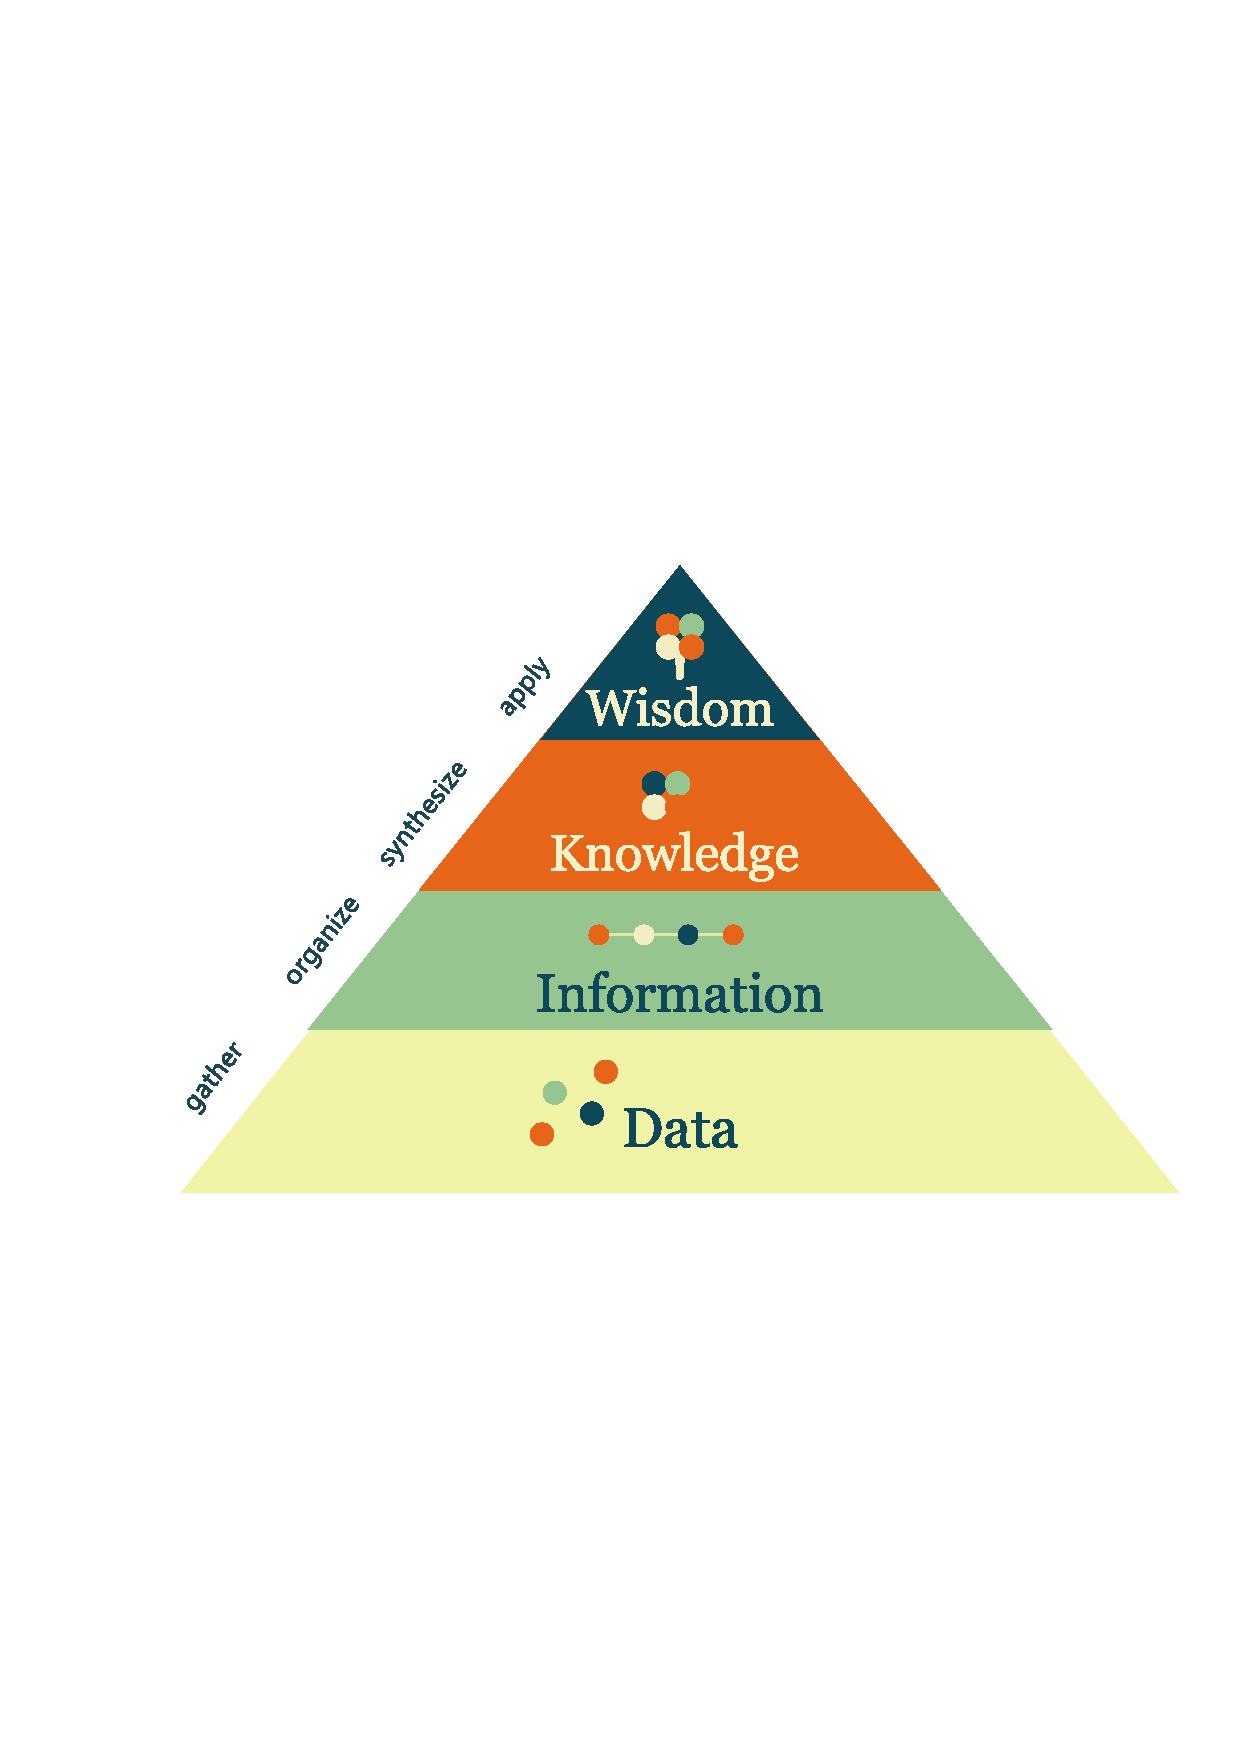
\includegraphics[trim=0 260pt 0 260pt, clip, width=0.75\textwidth]{parts/foundations/images/dikw_pyramid.pdf}
    \caption{Conceptual representation of DIKW pyramid.}
    \label{fig:dikw}
\end{figure}


The relevance of this framework in the context of digitalization lies less in the existence of a strict hierarchy than in the progressive transformation it emphasizes. The increasing value of data derives from the ability to move beyond its mere collection and towards its interpretation and use. Operational databases provide the means to capture observations reliably; analytical infrastructures organize and contextualize them; analytical methods extract patterns and models; and decision-support mechanisms make the resulting knowledge useful for planning and action.

This evolution also changed the requirements imposed on the infrastructures supporting data processing. As long as the principal objective was the reliable recording of operational events, relatively stable schemas and transaction-oriented workloads were sufficient. As data began to be integrated across systems and analyzed historically, systems had to support larger datasets, increasingly complex queries, heterogeneous sources, and transformations between operational and analytical representations.

The growing diversity of digital sources further amplified these requirements. Web applications, distributed software systems, multimedia repositories, machine logs, and eventually sensor infrastructures generated data with substantially greater volume and variety, often without the rigid structures traditionally associated with transactional systems. Data management therefore progressively moved beyond centralized relational databases towards scalable distributed infrastructures capable of storing and processing heterogeneous, semi-structured collections of data.

NoSQL solutions, data lakes and big data platforms emerged in response to these requirements, providing mechanisms for the large-scale storage and distributed processing of heterogeneous data. Later data lakehouse architectures attempted to combine the flexibility of large-scale data storage with stronger transactional, performance, and governance capabilities. Across these developments, a common trend can be observed: as the amount and diversity of data increased, the computational infrastructure had to become increasingly capable of integrating and processing data that could no longer be treated as a small collection of homogeneous, stable records. Consequently, data management in terms of integration and governance became just as important, if not more so, than the ability to efficiently store and retrieve data.

At the same time, the temporal dimension of data became increasingly important. Traditional analytical workloads were predominantly retrospective. They aimed to explain historical behaviour, compare past states, and identify patterns in accumulated records. As digital systems began to generate data continuously, however, a new requirement emerged: information had to be processed while the underlying process was still unfolding.

Streaming architectures consequently introduced a complementary computational model in which data could be ingested, transformed, enriched, and analyzed continuously rather than exclusively through periodic batch execution. The evolution from batch-oriented to continuous processing reduced the temporal distance between the observation of an event and the computational response to it.

This change was particularly relevant for predictive analytics. Once historical data could be combined with statistical and machine-learning methods, information systems were no longer limited to describing what had happened. They could estimate future states, identify emerging conditions, forecast demand, predict failures, and support decisions under uncertainty. The analytical objective consequently shifted from retrospective description towards anticipation.

More recent advances in artificial intelligence extend this trajectory further. Large-scale machine-learning systems can derive increasingly complex representations and predictions from heterogeneous data, while generative AI systems can synthesize information and interact with it through increasingly flexible interfaces. Emerging agentic AI systems further combine these capabilities with reasoning, planning, tool use, and execution. In this setting, data is not merely an input to an isolated analytical process. It becomes part of the context upon which a computational system bases decisions and actions.

The resulting progression can therefore be understood as a gradual reduction in the temporal and conceptual distance between data and action. Early information systems primarily recorded what had happened. Analytical systems transformed accumulated records into information and knowledge. Predictive systems increasingly estimated future states. Agentic AI systems can use such information to support decisions and, in some contexts, participate directly in their execution.

This progression continuously raises the requirements imposed on data management. The larger and more heterogeneous the datasets become, and the closer computation moves towards operational decision making, the more important it becomes that data can be obtained, processed, and interpreted in a timely and reliable manner. The relevant challenge is consequently no longer only how to store more data or process it faster, but how to manage data in ways that preserve its usefulness as it moves across increasingly heterogeneous computational environments.

While continuous data collection and storage techniques have become increasingly mature, the integration and governance of heterogeneous data needed to continuously derive meaningful knowledge and support timely action remain open challenges.

% =========================================================================
\section{From Information Systems to Cyber-Physical Systems}

\label{sec:dss_to_cps}

% =========================================================================

The evolution of data-intensive information systems was accompanied by a progressive expansion of the physical processes that could be digitally observed and computationally managed. Early information systems primarily operated on data generated by organizational activities and transactions. As analytical capabilities matured, these data were increasingly used to support monitoring, planning, and decision making through Business Intelligence, analytical models, and Decision Support Systems (DSS).

The emergence of the Internet of Things (IoT), together with advances in sensing technologies, embedded electronics, communication networks, and distributed computing, progressively extended this computational capability beyond traditional enterprise applications. Physical assets and environments could increasingly be equipped with sensors and connected devices capable of continuously acquiring and transmitting measurements about their state. In the context of Industry~4.0, this pervasive instrumentation became an important enabler of increasingly connected and data-intensive industrial environments.

The availability of continuous physical observations introduced a fundamental change in the relationship between information systems and the processes they represented. Instead of operating primarily on data generated by human or organizational activities, computational infrastructures could increasingly incorporate observations originating directly from the physical processes being monitored. These observations could then be integrated with information systems, analytical models, and decision mechanisms to support increasingly timely responses.

This convergence between information processing and physical processes provided the basis for the development of \textbf{Cyber-Physical Systems} (CPS). CPS are systems in which computational and communication capabilities are tightly integrated with physical processes through sensing and actuation, establishing feedback interactions between their cyber and physical components \cite{lee2008,nist_cps}. In a CPS, computational processes do not merely represent or analyze a physical process, but can continuously observe its state and, through appropriate control mechanisms, influence its evolution. Sensing, computation, communication, and actuation therefore form an integrated loop connecting the physical and cyber domains.

The transition from conventional Information Systems and DSS to CPS can therefore be understood as a change in the role and temporal relevance of data within the computational loop. In traditional information systems, data often describe organizational activities whose relevant state changes on timescales compatible with human decision making and periodic information processing. Pervasive sensing and CPS extend this model to physical processes characterized by substantially different dynamics. Some processes may evolve relatively slowly, allowing observations to be collected, aggregated, and analyzed over relatively long periods. Others may change continuously or rapidly, requiring observations to be processed and decisions to be taken within increasingly short time windows.

This distinction introduces an important temporal dimension to data-intensive systems. As the rate at which physical processes evolve increases, the interval available between observing a system, processing the corresponding information, and taking an appropriate decision becomes progressively smaller. The value of an observation may therefore depend not only on its accuracy or availability, but also on whether it can be acquired, transmitted, interpreted, and acted upon within the relevant temporal window of the physical process. Data management consequently becomes increasingly intertwined with the operational requirements of the systems that generate and consume the data.

At the same time, pervasive digitalization makes physical processes increasingly observable through multiple and independently developed systems. A single physical entity may be described through sensor measurements, information maintained by enterprise systems, engineering models, historical observations, simulation results, and analytical outputs. These sources may differ in structure, semantics, granularity, temporal resolution, and purpose. The challenge is therefore not only to acquire physical observations, but also to maintain meaningful relationships among the different forms of information describing the same physical entity or process.

This requirement motivates a further abstraction of the relationship between physical processes and their digital representations. Rather than treating physical observations only as inputs to individual monitoring or control loops, digital systems can maintain persistent virtual representations associated with physical entities or processes. Such representations can combine information originating from different sources and from different stages of the entity's lifecycle, providing a computational view that can be used for monitoring, analysis, simulation, prediction, and coordination.

This is the conceptual space in which the Digital Twin paradigm has emerged. Digital Twins and CPS should not, however, be understood as successive technologies in a simple evolutionary chain. Rather, they represent complementary perspectives on the digitalization of physical processes. CPS focus on the integration of computation, communication, sensing, and actuation with physical processes, enabling computational systems to observe and influence their operation. Digital Twins focus on maintaining and exploiting digital representations of physical entities or processes, potentially integrating information from multiple systems and over extended periods of their lifecycle. A CPS may therefore incorporate one or more Digital Twins as part of its computational capabilities, while a Digital Twin may operate as a component of a larger cyber-physical environment without itself constituting a complete CPS.

From this perspective, Digital Twins extend the role of digital information beyond the immediate feedback loops of individual cyber-physical systems. A Digital Twin can maintain a persistent and information-rich representation of an entity, combining current observations with historical data, contextual information, models, and analytical results. This representation can subsequently be exploited for purposes that extend beyond real-time control, including simulation, prediction, optimization, lifecycle management, and coordination with other digital representations.

The increasing integration of pervasive sensing, CPS, and Digital Twins therefore changes both the scale and the temporal characteristics of data-intensive systems. Physical processes can be observed continuously, their digital representations can be maintained over time, and computational decisions can increasingly be made within narrow temporal windows. At the same time, these representations may depend on information produced by multiple systems and serving different purposes. The resulting data-management problem is consequently characterized not only by increasing data volumes and velocities, but also by the need to manage heterogeneous information that is continuously produced, consumed, and transformed across interconnected computational and physical processes.

These characteristics motivate the need for data management approaches and software infrastructures capable of supporting Digital Twins as components of larger, interconnected ecosystems. In particular, the ability to integrate information originating from different sources, while respecting the temporal and operational requirements of the physical processes they represent, becomes a fundamental requirement for moving from isolated Digital Twins toward interoperable Digital Twin ecosystems.


% =========================================================================

\section{The Role of Data in a Digital Society}

\label{sec:role_of_data}

% =========================================================================

The developments described above have progressively transformed data from an operational by-product into a strategic resource of the digital economy. Data is now continuously or repeatedly generated by enterprise systems, software applications, connected devices, industrial equipment, and physical infrastructures. Its increasing economic and technological importance is well captured by the expression \emph{``data is the new oil''}\footnote{The phrase is widely attributed to British mathematician and data scientist Clive Humby\cite{humby2006data}.}.

The metaphor is particularly useful because the value of oil does not arise from extraction alone. Crude oil must be transported, refined, and processed before it becomes a useful product. Data follows a similar principle. Raw data has limited value in isolation: it must be collected, stored, transformed, integrated, and interpreted before it can contribute to information, knowledge, and ultimately action. Databases, data warehouses, distributed data platforms, stream-processing infrastructures, and analytical methods can therefore be viewed as the infrastructure through which raw data is progressively transformed into something that can be used.

The scale of this resource has grown rapidly. IoT Analytics estimates 18.5 billion connected IoT devices in 2024 and 21.1 billion by the end of 2025, with approximately 39 billion forecast for 2030\footnote{IoT Analytics, ``State of IoT: Number of Connected IoT Devices,'' \url{https://iot-analytics.com/number-connected-iot-devices/}, updated October 2025.}. Beyond the physical volume of data generated, its economic relevance is also measurable. The European Data Market Study 2024--2026 estimates the EU27 data market at approximately EUR~90 billion in 2024, up from EUR~82 billion in 2023, while the broader data economy---including the direct and indirect economic impacts of data---reached approximately EUR~579 billion in 2024, with a baseline projection reaching approximately EUR~815 billion by 2030 \cite{eudatamarket2024}.

These figures also highlight an important distinction: the value of data does not derive simply from its existence or volume, but from the capability to make it useful. The same principle has accompanied the evolution of information systems throughout the previous decades. Data Warehouses transformed operational records into analytical information; Big Data platforms enabled the management of large heterogeneous datasets; streaming infrastructures enabled continuous processing; and analytical methods transformed accumulated observations into models and knowledge.

The oil metaphor has, however, increasingly been challenged on precisely the dimension of sustainability it seems to evoke. Oil is a finite, extractive resource whose consumption is inherently exhaustible; data, by contrast, is typically assumed to be effectively limitless and immaterial, infinitely copiable at negligible marginal cost, and detached from any physical substrate that could itself be depleted. Taffel critically examines this assumption, arguing that the metaphor implicitly frames digital technologies as clean, renewable, and sustainable, whereas an infrastructural analysis of the material conditions underpinning data reveals a rather different picture: the substantial quantities of energy, minerals, and fossil fuels required to sustain global data infrastructure, together with the environmental costs of its manufacturing and disposal \cite{taffel2021}. From this perspective, the metaphor does not merely simplify; it actively obscures the environmental footprint of the digital economy it purports to describe.

The rapid growth of data centres and, more recently, of artificial intelligence workloads has made this material dimension increasingly difficult to ignore. The International Energy Agency, in a report explicitly examining the relationship between energy demand and artificial intelligence, estimates that data centres consumed approximately 415~TWh of electricity in 2024, around 1.5\% of global electricity consumption, and projects consumption to reach approximately 945~TWh by 2030 in its base case, representing just under 3\% of global electricity demand. The report attributes a substantial share of this growth to the rapid expansion of AI-specific data centres and workloads \cite{iea2025}. In parallel, the 2024 United States Data Center Energy Usage Report estimates approximately 66 billion litres of direct water consumption by US data centres in 2023, compared with 21.2 billion litres in 2014 \cite{shehabi2024}.

These figures make clear that digitalization is not detached from the physical world: digital infrastructures depend on physical resources, energy, communication networks, hardware, and facilities, and their sustainability cannot be taken for granted simply because data itself appears immaterial.

The increasing collection and exploitation of data also raises a further set of concerns, distinct from its material or economic dimensions: questions of privacy, security, ownership, and governance over who may access, combine, and repurpose it. These concerns become more pressing as data increasingly moves across organizational boundaries and independently developed systems, a tendency this thesis returns to when discussing the data governance mechanisms required for Digital Twin Ecosystems in \Cref{chap:data_oriented_perspective}. The greater the scale and pervasiveness of digital observations, the greater the importance of being able to determine and trace how data is collected, processed, shared, retained, and reused.

The increasing importance of data is also accompanied by a change in the type of value expected from it. Historical data remains fundamental for identifying patterns and training models, but modern AI systems increasingly use data to estimate future states, generate recommendations, and support decisions. Emerging agentic AI systems further extend this trajectory by combining information retrieval, reasoning, tool use, and increasingly autonomous execution.

This development does not eliminate the underlying data-management problem. On the contrary, it makes the quality and usability of the data substrate increasingly important. Systems capable of reasoning or acting upon information depend on data to be interpreted correctly, placed in context, and accessed in a timely manner, properties that are often clustered into the data quality concept. As the outputs of computational systems become increasingly connected to operational decisions and physical processes, the consequences of poorly managed or isolated data also become more significant.

The evolution described in this chapter can therefore be read as a progression from data as record to data as resource, and from data as passive representation to data as an active component of computational decision loops -- with each transition raising, rather than resolving, the underlying requirement to integrate and govern the resulting data reliably. Digital Twins represent the most recent stage of this progression, maintaining persistent representations of physical entities that draw on multiple sources over their operational lifetime; the specific challenges this raises for independently developed Digital Twins are examined in detail in the next chapter.

This requirement is set to become more pressing, not less. As growing numbers of Digital Twins, and of digital systems more generally, are expected to coexist and collaborate rather than operate in isolation, the data they produce and consume increasingly needs to be shared, reconciled, and jointly interpreted across systems that were never designed together. Meeting this requirement calls for governance mechanisms substantially stronger than those sufficient for a single, self-contained system -- covering the quality, provenance, semantics, and access of data as it moves across organizational and technical boundaries. This is not a concern confined to Digital Twins. The same dependence on well-integrated, well-governed data underlies the emerging generation of AI agents: systems that retrieve information, reason over it, and act with increasing autonomy are only as reliable as the data they draw upon. An agent reasoning over incomplete, inconsistent, or poorly governed data does not merely risk a wrong answer; it risks acting on one. Ensuring the integration and governance of data is therefore not a narrow architectural concern, but an increasingly general precondition for extending autonomous computational systems into the physical world without their errors compounding unchecked.

The challenge emerging at this stage is consequently not only how to collect, store, or process increasingly large amounts of data, but how to provide the architectural and data foundations that make its integration and governance possible across independently developed systems.

The following chapters build on this observation. First, the Digital Twin paradigm is examined in greater detail, including its definitions, characteristics, and current implementations, in order to identify the requirements that distinguish Digital Twin environments from traditional information systems. These requirements motivate a subsequent shift towards a data-oriented perspective, in which data models, architectures, and the mechanisms used to structure and manage Digital Twin data become central to achieving interoperability among independently developed Digital Twin systems.


\chapter{Digital Twins}
\label{chap:digital_twins}
The evolution of digital systems described in the previous chapter provides the technological and conceptual context in which the Digital Twin paradigm has emerged. Increasing sensing capabilities, pervasive connectivity, distributed computing, and continuous data processing have made it possible to establish increasingly rich and persistent digital representations of physical entities and processes. Digital Twins build upon these capabilities by connecting physical systems with digital counterparts that can be used for monitoring, analysis, simulation, prediction, optimization, and decision support.

Despite the growing adoption of the term, however, Digital Twin remains a broad and heterogeneous concept. Different communities and application domains have proposed distinct definitions, architectures, and implementation approaches, often reflecting specific technological or operational requirements. This diversity has enabled the development of highly specialized solutions, but has also contributed to a fragmented landscape with limited interoperability between independently developed Digital Twin systems. As a result, the potential benefits of Digital Twins are often constrained by the difficulty of sharing and reusing information across different systems, applications, and domains.

This chapter examines the Digital Twin paradigm from this perspective. It first discusses the historical development of the concept and the heterogeneous interpretations that have emerged around its definition. It then examines reference architectures and the properties commonly associated with Digital Twins, highlighting the increasing complexity of the models, data, and computational capabilities involved. Building on this architectural discussion, it characterizes the data that Digital Twins produce and consume, and the requirements that follow from its unique characteristics. The discussion subsequently turns to the main challenges emerging from the proliferation of Digital Twin solutions. Finally, the chapter considers interoperability and standardization as emerging requirements for moving from isolated Digital Twin implementations towards interconnected Digital Twin ecosystems.

% =========================================================================

\section{History and Definition}
\label{sec:history-and-definition}
% =========================================================================
The Digital Twin concept origins are traced to Michael Grieves' work on Product Lifecycle Management (PLM)~\cite{grieves2014digital} at the beginning of the 2000s, where it was conceived as a virtual representation of a product throughout its lifecycle. The original conceptualisation introduced three fundamental components that characterize a DT, as also shown in \Cref{fig:grieves_dt}:
\begin{itemize}
    \item a \textit{physical space} and its products;
    \item a \textit{virtual space} with virtual representations of the products;
    \item a \textit{connection} between the two spaces, entailing an information flow between the two entities.
\end{itemize}

\begin{figure}[ht]
    \centering
    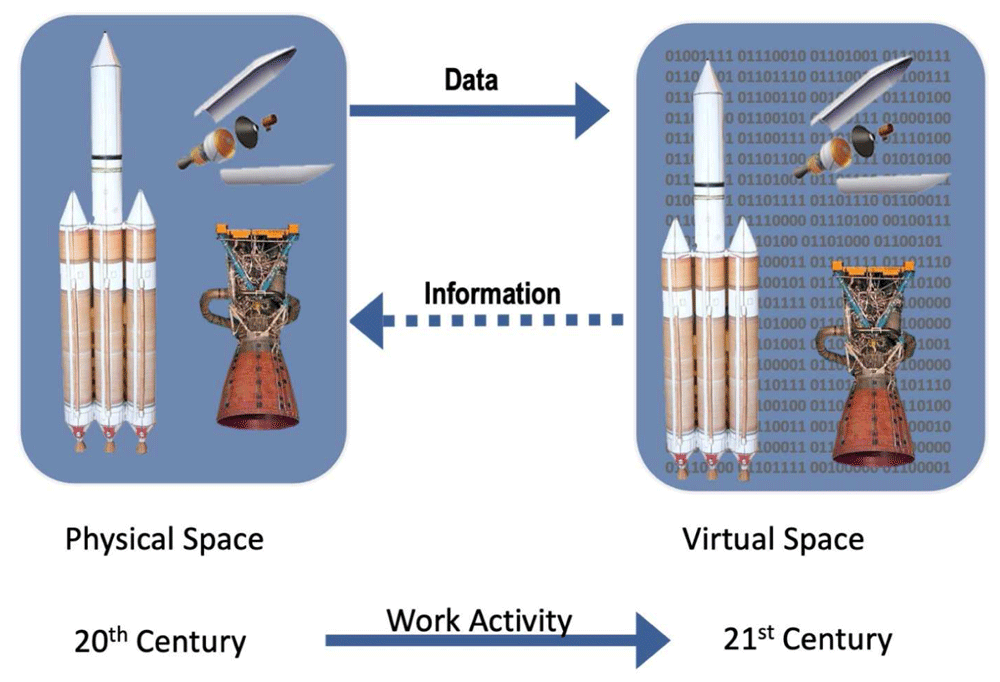
\includegraphics[width=0.65\textwidth]{parts/foundations/images/dt_model_grieves.png}
    \caption{The original DT conceptual model by Grieves, from~\cite{grieves2014digital}} 
    \label{fig:grieves_dt}
\end{figure}

Grieves' early-2000s work is generally regarded as the conceptual origin, while subsequent contributions associated the concept with the term \emph{Digital Twin} and extended it to aerospace and other engineering domains \cite{grieves2002,glaessgen2012,wuni2026}. 

This distinction is important because it places the relationship between the physical and digital spaces at the centre of the concept. The Digital Twin was conceived not merely as a model that could represent a physical object, but as a digital representation connected to it through an ongoing flow of information. In the original formulations, this connection enabled data describing the physical system to be incorporated into the virtual representation, while the information generated within the virtual space could be used to inform decisions concerning the physical system \cite{grieves2014digital,glaessgen2012}.

The subsequent diffusion of the concept was closely related to the development of Industry~4.0, the Internet of Things, industrial connectivity, and data analytics. As physical systems became increasingly instrumented and connected, the continuous acquisition of operational data made it possible to maintain increasingly dynamic digital representations. Digital Twins consequently moved beyond their original product-lifecycle-oriented formulation and were adopted across manufacturing, aerospace, energy, buildings, transportation, healthcare, smart cities, and other domains \cite{qi2021,liu2021,tao2022}.

The growth of the research field reflects this broad diffusion. Tao et al. reported more than 1,000 Digital Twin-related papers per year for three consecutive years beginning in 2019, with 2,934 papers published in 2021 \cite{tao2022}. More recent analyses show an even stronger increase. Wuni et al., analysing scientific and practitioner literature up to 2024, report a substantial growth in Digital Twin publications and identify the last decade as the period in which the vast majority of currently circulating definitions were introduced \cite{wuni2026}. The resulting literature is correspondingly broad, spanning multiple disciplines, application domains, technological approaches, and interpretations of the Digital Twin concept.

This rapid expansion has also created a conceptual problem. As the term has been adopted by communities with different backgrounds and objectives, Digital Twin has increasingly become an umbrella concept encompassing substantially different systems. Different studies may use the same term to describe a simulation model, a three-dimensional representation, a monitoring system, a predictive model, or a fully connected cyber-physical system. Several reviews have therefore identified the lack of a universally accepted definition as one of the persistent challenges of the field \cite{barricelli2019,jones2020,fuller2020,wuni2026}.

\begin{figure}[ht]
    \centering
    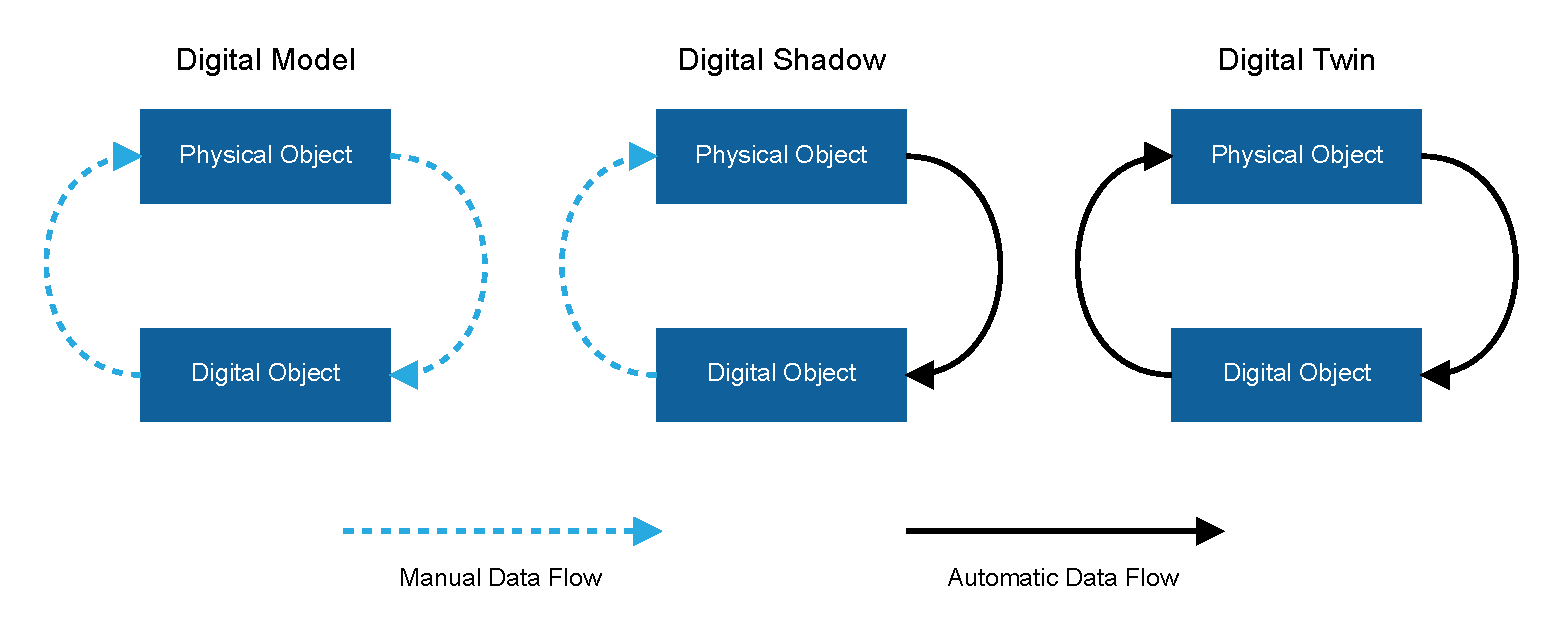
\includegraphics[scale=0.5]{parts/foundations/images/dmdsdt.pdf}
    \caption{Differences between Digital Model, Digital Shadow, and Digital Twin, adapted from Kritzinger et al.~\cite{kritzinger2018}.}
    \label{fig:dtdsdm}
\end{figure}

A particularly useful distinction in this context is the one between a \emph{Digital Model} (DM), a \emph{Digital Shadow} (DS), and a \emph{Digital Twin}, as shown in \Cref{fig:dtdsdm}. Kritzinger et al. introduced this distinction according to the degree and direction of information exchange between the physical and digital entities, a classification subsequently adopted by several reviews and studies \cite{kritzinger2018,fuller2020}. A DM represents a physical entity without an automated connection to it. Changes in the physical system therefore do not automatically propagate to the model, and changes in the model do not automatically affect the physical system.

A DS introduces an automated, but one-directional, connection. Information about changes occurring in the physical system is automatically transferred to the digital representation. The digital representation therefore provides an updated view of the physical system, but does not necessarily influence it automatically. A Digital Twin extends this relationship to bidirectional exchange: changes in the physical system can update the digital representation, while information or decisions generated in the digital space can affect the physical system \cite{kritzinger2018,fuller2020}.

The progression from DM to DT is not primarily determined by the complexity or fidelity of the digital representation, but by the nature and importance of the connection established between the physical and digital entities. A highly detailed three-dimensional simulation that is disconnected from its physical counterpart is therefore not necessarily a Digital Twin, while a less visually sophisticated representation may qualify as one if it is continuously connected to the physical system through an appropriate data flow.

The distinction also highlights the central role played by data in the Digital Twin concept. The transition from DM to DS is enabled by the introduction of an automated data flow, while the transition from DS to DT requires the ability to exchange information in both directions \cite{kritzinger2018,fuller2020}. Communication and data exchange are therefore not merely implementation details; they constitute one of the mechanisms through which the relationship between the physical and digital spaces is established.

Recent systematic analyses provide further evidence of the persistent difficulty of maintaining this conceptual distinction. Wuni et al. analysed 358 definitions from scientific and practitioner sources and found that 66.48\% captured the physical entity, its virtual counterpart, and a persistent bidirectional data and information flow, whereas 33.52\% described entities that, according to their classification, were more appropriately understood as Digital Models \cite{wuni2026}. The analysis also found that terms such as \emph{data}, \emph{information}, \emph{real-time}, \emph{representation}, and \emph{entity} are frequently present in Digital Twin definitions, while terms describing the continuous exchange itself are comparatively less represented \cite{wuni2026}.

This result is particularly relevant to the evolution of the concept. The literature has increasingly recognized that a Digital Twin cannot be reduced to a static representation. Nevertheless, the different formulations used to describe the connection, synchronization, and exchange between physical and virtual entities indicate that the data flow remains interpreted in substantially different ways across the literature. The conceptual core of the Digital Twin is therefore increasingly associated with continuity and synchronization, while the concrete mechanisms through which these properties are modelled and implemented remain strongly dependent on the application domain.

The definition of Digital Twin adopted in this thesis follows this core interpretation.

\begin{quote}
\textit{A Digital Twin is a digital representation of a physical entity or process, continuously connected to its physical counterpart through a bidirectional exchange of information. This enables the digital representation to stay updated with the physical state, while allowing insights generated in the digital space to trigger decisions and actions that directly affect the physical entity.}
\end{quote}

The digital representation may depend on multiple information sources, interact with other digital entities, and expose information that could be relevant to other applications. The more Digital Twins are deployed across interconnected domains, the more important the mechanisms governing their interaction become.

\section{Reference Architectures and Properties}
\label{sec:ref-arch}
% =========================================================================

The increasing adoption of Digital Twins has led to the development of several conceptual models and reference architectures intended to describe their main components and relationships. Although no single architectural representation has emerged as universally adopted, different proposals progressively extend the original conceptualization of the Digital Twin by introducing additional dimensions related to modelling, data, communication, and services \cite{qi2021,tao2022,liu2021}. These models provide useful abstractions for understanding how Digital Twins are structured and how their different components contribute to their operation.

The original formulation introduced by Grieves provided a deliberately simple conceptual representation based on three elements: a physical entity in the physical space, its virtual representation in the virtual space, and a connection enabling information exchange between the two \cite{grieves2014digital}. In this view, the virtual representation provides the digital counterpart of the physical entity, while the connection establishes the relationship through which information can be exchanged. The model therefore captures the fundamental physical--digital relationship underlying the Digital Twin concept.

As Digital Twin applications evolved beyond their original product-lifecycle context, more detailed architectural representations were proposed. One of the most widely referenced models is the five-dimensional Digital Twin model introduced by Tao et al., which extends the original three-part conceptualization by explicitly identifying five dimensions: \textit{physical entity}, \textit{virtual model}, \textit{connection}, \textit{data}, and \textit{service} \cite{tao2019,qi2021}. The model is illustrated in \Cref{fig:tao_dt}.

\begin{figure}[ht]
    \centering
    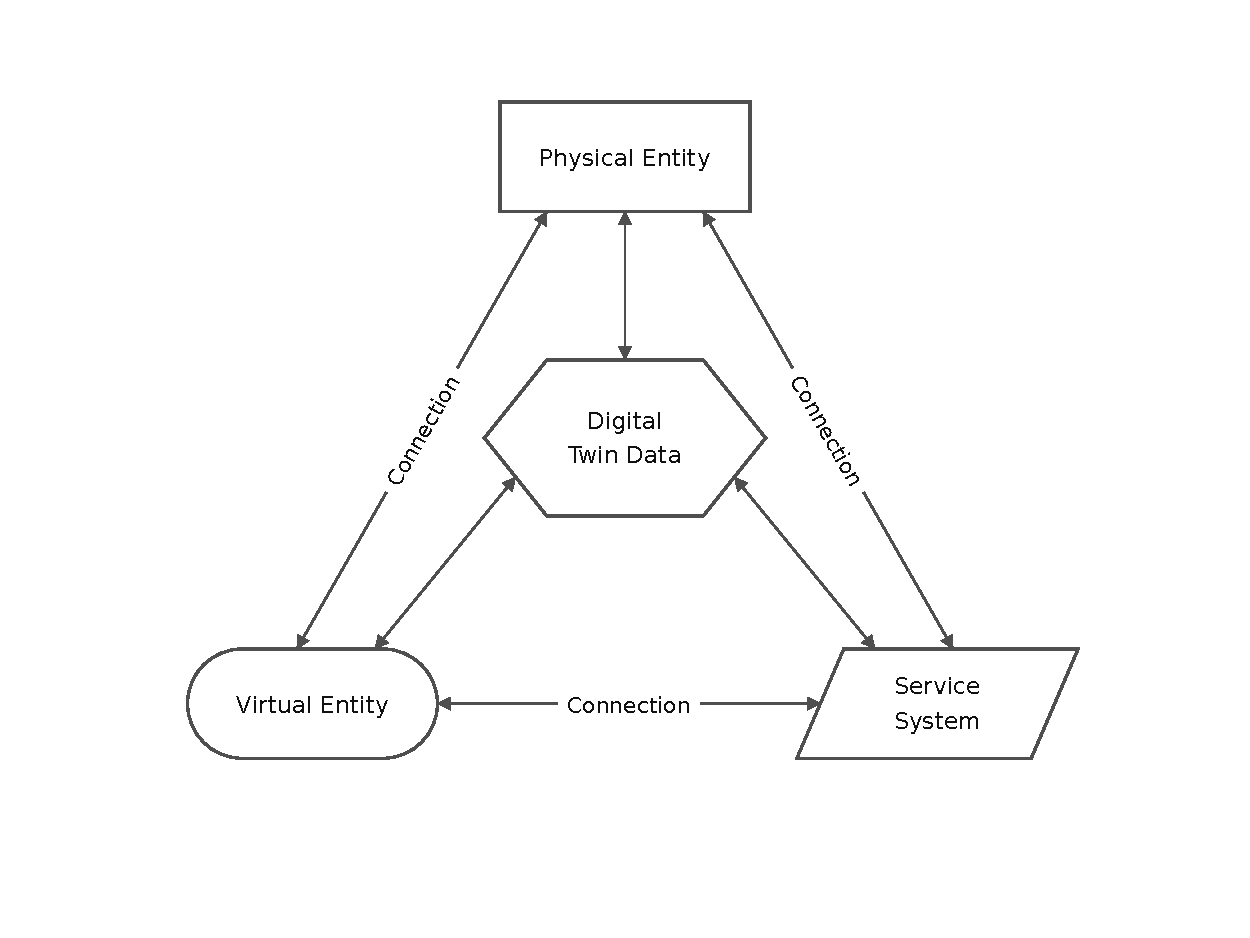
\includegraphics[scale=0.5]{parts/foundations/images/5dim_dt.pdf}
    \caption{Five-dimensional Digital Twin model, adapted from Tao et al.~\cite{tao2019,qi2021}.}
    \label{fig:tao_dt}
\end{figure}

The five-dimensional model provides a more comprehensive architectural view of a Digital Twin. The \textit{physical entity} represents the real-world object, system, or process being twinned, while the \textit{virtual model} provides its digital representation. The \textit{connection} establishes the communication between the physical and virtual spaces, enabling the exchange of information. The \textit{data} dimension captures the information generated, collected, and processed throughout the operation of the Twin, while \textit{services} represent the functionalities offered through the Digital Twin.

Within this model, the virtual representation is not necessarily limited to a single type of model. Tao et al. distinguish geometric, physical, behavioural, and rule models as complementary dimensions that can be combined to represent different aspects of the physical entity \cite{tao2022}. Geometric models describe the shape and structural characteristics of an entity; physical models capture relevant physical properties and constraints; behavioural models describe its dynamic evolution; and rule models incorporate rules, historical information, and domain knowledge. Depending on the application, these models can support simulation, prediction, optimization, diagnosis, and other computational functions.

The explicit introduction of data as a separate dimension, and specifically placed at the core of the architecture,  is particularly relevant to the evolution of Digital Twins. In the original three-component formulation, data was implicitly associated with the connection between the physical and virtual spaces. In the five-dimensional model, it is instead represented as an independent and pivotal architectural element connecting the physical entity, virtual model, connection, and services \cite{qi2021,tao2022}.

Data is therefore involved throughout the operation of a Digital Twin. Measurements and observations produced by the physical entity can be collected and used to update its virtual representation. Historical information can complement current observations, while data-driven and model-based techniques can transform these inputs into higher-level information and knowledge. The resulting outputs can support services such as monitoring, simulation, prediction, optimization, and decision making \cite{qi2021,tao2022}. Finally, outputs produced within the virtual reèresentation can in turn be used to determine actions affecting the physical entity.

As shown in numerous research articles, the diversity of application domains has consequently resulted in a wide range of Digital Twin architectures and implementations. Tao et al. reviewed 284 publications on Digital Twin models and found that almost half concerned manufacturing applications. Energy represented 35 publications and aerospace 20, while further applications were identified in areas such as engineering construction, cities, healthcare, transportation, and environmental systems \cite{tao2022}. This distribution illustrates the progressive diffusion of the concept from its initial engineering and manufacturing context towards a much broader set of application domains.

Architectural variation also emerges from the scale of the physical systems being represented. Tao et al. distinguish between unit-level, system-level, and System-of-Systems (SoS)-level Digital Twin models \cite{tao2022}. At the unit level, a Twin may represent an individual component or piece of equipment. At the system level, it may represent a production line, aircraft subsystem, building, or other integrated system composed of multiple components. At the SoS level, the Digital Twin represents a collection of interacting systems whose behaviour depends on the relationships between their constituent parts.

This hierarchical perspective is particularly relevant to the architecture of complex Digital Twin Environments (DTE).
%
The concept of DTE traces back to Grieves~\cite{Grtz2026}, who envisioned aggregating homogeneous DT instances to observe population-level behaviors and trends across identical products. In contrast, the modern framing of a Digital Twin Ecosystem (DTE) is largely shaped by the UK's National Digital Twin programme.
%
Under this paradigm, the National Digital Twin is defined as “an ecosystem of digital twins and the protocols by which they can be integrated securely and resiliently”~\cite{dtarch}. 
%
A Digital Twin at one level may therefore coexist with other Twins representing related entities at different levels of abstraction. In a manufacturing environment, for example, individual machines may be represented by dedicated Digital Twins, while a production line may be represented at a higher level by a Twin that considers the interactions among those machines. Similar hierarchical relationships can be found in other domains, such as aerospace, healthcare, and urban systems \cite{tao2022}.

Recent reference architectures have increasingly conceptualized the Digital Twin not as a tailored, self-contained entity, but as a modular platform component governed by service-oriented principles. Aligning with this perspective, Aheleroff et al. \cite{AHELEROFF2021101225} proposed a \emph{Digital Twin as a Service} (DTaaS) reference model for Industry 4.0. Their work highlights the necessity of abstracting DT functionalities into scalable, cloud-based services to support complex system integration across a large number of assets. Crucially, this DTaaS approach acts as an architectural blueprint: rather than dictating a monolithic structure, it identifies the mandatory infrastructural modules required to operate a DT. By standardizing these core components into composable building blocks, the architecture empowers developers to flexibly assemble, instantiate, and scale customized Digital Twins. Consequently, the development focus shifts from engineering isolated systems from scratch to leveraging a shared, service-oriented infrastructure that inherently fosters standardization and interoperability.

Across these different approaches, the specific technologies and internal structures may vary considerably, but several architectural elements recur: a physical entity, a digital representation, mechanisms for exchanging information between the two, data supporting the representation and its operation, and services built on top of the available models and information. The balance among these elements depends strongly on the domain, the characteristics of the physical system, and the intended functionality of the Digital Twin.

The literature therefore presents the Digital Twin not as a single architectural pattern, but as a family of related architectural abstractions. The original three-component model provides a conceptual foundation centered on the physical--digital relationship, while subsequent models introduce additional dimensions to capture the data, models, and services required by increasingly sophisticated implementations. In particular, the explicit introduction of data as an architectural dimension represents an important step in the evolution of the concept, reflecting the increasing role of information in maintaining, operating, and exploiting Digital Twins. Having recurred, in every reference architecture discussed above, as the element connecting the physical entity, its virtual representation, and the services built on top of it, data deserves to be examined in its own terms as the basis for the data-oriented perspective developed in the remainder of this thesis.

\section{Challenges and Opportunities}

\label{sec:challenges}

The increasing adoption of Digital Twins across different application domains introduces significant opportunities for monitoring, analysis, simulation, optimization, and decision support. At the same time, the current state of development of Digital Twins presents several challenges related to their increasing \textit{complexity} and wide \textit{heterogeneity}. In terms of heterogeneity, DTs may differ with respect to the physical systems they represent, the goals they pursue, the data they rely on, and most notably, the technologies and architectures used for their implementation.
%
Some of these differences are the result of the limited degree of \textit{standardization} achieved so far, despite the research community having strongly advocated for greater standardization efforts over the last decade \cite{wang2022standards,wuni2026}.
%
While the number of publications related to DTs has increased extremely rapidly, the literature shows that some studies still fail to provide a clear definition of the DT concept and consequently, at least partially, fail to reflect its essential characteristics in their implementations. Others provide definitions that are not consistent with one another \cite{wuni2026,tao2022}.
%
The lack of standardization also hinders the development of frameworks, reference architectures, and platforms capable of supporting the development of DTs in a consistent and modular way.
%
Furthermore, if standardization is already a challenge within individual DTs, its absence becomes even more relevant when considering more complex scenarios such as DTEs, in which multiple DTs are expected to coexist and meaningfully interact.

The meaningful interaction required within DTEs introduces a further challenge related to \textit{interoperability}. Independently developed DTs need to be able to communicate and exchange information in a way that is meaningful for all the systems involved. This requires not only a technical connection between the systems, but also a shared understanding of the exchanged information, including its semantics and context. Interoperability is therefore a multi-level challenge encompassing technical, syntactic, and semantic aspects, and requiring mechanisms to manage differences between independently developed systems.

Heterogeneity and the resulting lack of coordination between independently developed Digital Twins are, in this sense, the root of the problem. Addressing them requires progress along two related fronts. \textbf{Standardization} is the primary lever available for this purpose: the definition of common principles, structures, and mechanisms that can provide shared foundations for developing and managing Digital Twins, thereby reducing unnecessary heterogeneity. \textbf{Interoperability} is the capability such foundations are meant to enable: the ability of different, independently developed Digital Twins to communicate, exchange information, and cooperate effectively. Standardization and interoperability are therefore closely related (the former is typically a precondition for the latter) but they address different aspects of the problem and, as discussed below, are not always achieved together.
%
These two dimensions will be discussed from two different perspectives: single Digital Twins and Digital Twin Ecosystems. The former primarily concerns the development of individual Digital Twins, while the latter concerns the interaction between multiple independently developed Digital Twins.

\subsection{Standardization}

At the level of an individual Digital Twin, standardization can provide a common foundation for its construction and management. Rather than defining every Digital Twin as a completely independent solution, standardized building blocks, architectural principles, and mechanisms can guide developers in assembling the components required by a particular application. Such standardization does not require all Digital Twins to have the same structure or capabilities. Instead, it can provide a common set of elements from which different Digital Twins can be constructed and tailored to their specific requirements.

At the level of a Digital Twin Ecosystem (DTE), the scope of standardization becomes broader. A DTE involves multiple Digital Twins that may have been developed independently and may rely on different technological solutions. Standardization can therefore concern the common foundations of the ecosystem itself, including the infrastructure, architectural principles, interfaces, and data representations that support the deployment and interaction of multiple Digital Twins. In this sense, standardization can reduce unnecessary differences between implementations and provide a common basis on which heterogeneous Digital Twins can coexist.

Wang et al. review the landscape of Digital Twin standardization efforts, consolidating contributions from organizations including the International Organization for Standardization (ISO), the International Electrotechnical Commission (IEC), the International Telecommunication Union (ITU), and the Institute of Electrical and Electronics Engineers (IEEE) \cite{wang2022standards}. Their review is framed around the five-dimensional Digital Twin model introduced by Tao et al., comprising the physical entity, virtual model, connection, data, and services \cite{tao2019,qi2021}. For the purposes of this thesis, two of these dimensions are particularly relevant: the \textit{connection}, which provides the infrastructural basis for communication and interaction, and \textit{data}, which constitutes the information exchanged and processed by the different components of the Digital Twin.

From an infrastructural perspective, standardization addresses the mechanisms through which Digital Twins and their components can connect and communicate. Common interfaces, communication protocols, service descriptions, and architectural principles can reduce implementation-specific dependencies and facilitate the integration of independently developed components. Wang et al. identify the lack of common references for Digital Twin architectures and communication mechanisms as an important obstacle to the interconnection of Digital Twin components and services across different systems and domains \cite{wang2022standards}. Standardization at this level therefore provides the technical foundations required for Digital Twin systems to communicate.

A second and complementary dimension concerns the data exchanged through these infrastructures. Digital Twins continuously produce, consume, and transform information originating from physical entities, models, sensors, information systems, and other computational services. Wang et al. identify several standardization requirements related to Digital Twin data, including the processing of heterogeneous data, the management of multi-source and multi-modal data, and mechanisms concerning data syntax, semantic mapping, and data exchange \cite{wang2022standards}. These requirements indicate that standardization cannot be limited to the mechanisms used to transport data; the representation and interpretation of the exchanged information are equally, if not more so, relevant.

These two dimensions of standardization, of the infrastructure used to connect Digital Twins, and of the data they exchange, do not exhibit the same degree of maturity. Communication and interface standards provide increasingly established mechanisms through which heterogeneous systems can connect, while data-oriented standards and semantic approaches are comparatively less developed \cite{wang2022standards}. This gap becomes especially relevant within a Digital Twin Ecosystem: while an individual Digital Twin can often rely on tightly coupled, internally consistent interfaces and data representations, a Digital Twin Ecosystem brings together systems designed around different assumptions, so that establishing a communication channel between them is only a first step. Standardizing that channel does not, by itself, guarantee that the information exchanged through it will be correctly interpreted by the receiving system.

From this perspective, standardization should not be understood as an attempt to impose a single implementation on all Digital Twins. Domain-specific models, technologies, and services may remain necessary to address the characteristics of individual physical systems. The objective is instead to identify and standardize the common elements at the boundaries between systems, allowing Digital Twins to retain their internal specialization while remaining capable of participating in a broader ecosystem. Achieving such common foundations can reduce the effort required to develop new Digital Twins, facilitate their integration, and enable the reuse of data and services across applications. It can also support the development of reusable frameworks and platforms capable of deploying and managing Digital Twins according to shared architectural principles.     However, providing common foundations does not, by itself, guarantee that independently developed Digital Twins can effectively work together. This motivates the following discussion, which considers interoperability as a distinct challenge in its own right.

\subsection{Interoperability}

Interoperability becomes particularly relevant at the level of the Digital Twin Ecosystem. When multiple Digital Twins are independently developed, they may rely on different architectures, interfaces, data representations, and terminology. The challenge is therefore to enable these systems to communicate seamlessly and to exchange information that can be correctly understood and used by the receiving system.

At the level of an individual Digital Twin, there is no interoperability problem in the sense of interaction between independently developed Digital Twins, since the system is considered in isolation. Internal components still need to interact with one another, but this is primarily a matter of designing and integrating the Digital Twin itself. Interoperability becomes a distinct concern when multiple Digital Twins are brought together within a DTE.

This distinction is important because interoperability does not simply mean connecting systems despite their differences. Rather, it concerns finding ways to integrate those differences so that independently developed systems can communicate and make meaningful use of the information exchanged between them. A system should not merely receive a message from another system; it should be able to understand what that information represents and use it within its own context.

This requirement becomes particularly important when Digital Twins exchange information that contributes to monitoring, analysis, or decision-making. Two systems may use different representations for the same physical phenomenon, and a successful interaction requires more than a technical connection between them. The receiving system must be able to interpret the exchanged information according to its intended meaning and context.

Recent literature has begun to characterize this problem more precisely, distinguishing between several levels at which interoperability between Digital Twins can be assessed and pursued. Acharya et al.~\cite{acharya2024interoperability}, surveying interoperability within Digital Twin deployments in cyber-physical systems, delineate distinct interoperability levels and examinTheir analysis proposes a framework of six such levels -- \textit{technical}, \textit{syntactic}, \textit{semantic}, \textit{pragmatic}, \textit{dynamic}, and \textit{organizational} -- ranging from the basic ability of Digital Twins to exchange messages over a common communication infrastructure, through agreement on a common structure and encoding for the exchanged data, up to the higher-level ability to agree on the meaning of the exchanged concepts and on the business or operational context in which they are used. For the purposes of this thesis, the technical, syntactic, and semantic levels are the most directly relevant, since they map most closely onto the software/data distinction followed here.
%
David et al. similarly review the challenges affecting interoperability among Digital Twins, together with the factors that have been found to contribute to successful interoperable deployments, and outline directions for future research on the topic \cite{david2024interoperability}. Both contributions confirm that achieving interoperability across independently developed Digital Twins requires more than establishing a technical connection between them.

A simple example makes the semantic level concrete: two Digital Twins monitoring similar physical processes may represent the same measured quantity, such as temperature, under different property names, units, or data structures. A compatible communication channel is sufficient to transmit the corresponding value from one system to the other, but it does not by itself guarantee that the receiving system correctly identifies what that value represents; establishing this correspondence is a matter of semantic, rather than merely technical or syntactic, interoperability.

Standardization and interoperability therefore address complementary aspects of the same underlying problem: the former provides shared architectural and data-related foundations for constructing Digital Twins and Digital Twin Ecosystems, while the latter concerns the ability of independently developed Digital Twins to exchange and meaningfully reuse each other's information once such foundations are in place. The following chapter examines this problem from the perspective of the data involved, characterizing the data that Digital Twins produce and consume and the mechanisms required to manage it consistently across independently developed systems.

\chapter{A Data Oriented Perspective}
\label{chap:data_oriented_perspective}
This chapter adopts a data-oriented perspective on the standardization and interoperability challenges discussed in the previous chapter. It first argues for treating the data and software dimensions of a Digital Twin as separable, complementary design concerns, and examines how the two challenges just discussed relate to this separation. It then characterizes the data that Digital Twins produce and consume, discussing the requirements that follow from the diversity of the domains in which Digital Twins are deployed. Finally, building on this characterization, it examines the architectural and semantic foundations required to support such data across individual Digital Twins and Digital Twin Ecosystems.

\section{Divide et Impera}

Digital Twins, and the platforms that support them, can be described along two complementary dimensions: a \textit{software} dimension, concerned with the applications, services, and infrastructural components through which Digital Twins are deployed, executed, and made accessible; and a \textit{data} dimension, concerned with the information that Digital Twins collect, process, store, and exchange. These two dimensions are not independent, but modular and complementary. Every software component of a Digital Twin, from the simplest monitoring dashboard to the most sophisticated simulation service, ultimately operates on data: it acquires it, transforms it, and produces new data to be stored and eventually consumed elsewhere. In this sense, the software dimension of a Digital Twin can be regarded as a layer of applications built on top of the data dimension, rather than as an independent architectural concern.

This observation motivates a deliberate decomposition of the problem. Rather than addressing the software and data dimensions jointly, and thereby risking the reproduction of the same fragmentation already observed in existing Digital Twin implementations, this thesis separates the two concerns and concentrates on the data dimension. This choice is not intended to diminish the relevance of software architectures, which remain necessary to deploy, orchestrate, and expose Digital Twin functionalities. It reflects, instead, the observation that many of the interoperability difficulties discussed in the previous chapter originate not from the diversity of software implementations per se, but from the heterogeneity of the underlying data: its models, schemas, semantics, and governance \cite{acharya2024interoperability,david2024interoperability}. Two Digital Twins built on entirely different software stacks can still interoperate if they share a common understanding of the data they exchange, whereas two Digital Twins built on the same software stack may fail to interoperate if their underlying data representations are incompatible.

This separation can be made more concrete by revisiting the standardization and interoperability challenges discussed in \Cref{sec:challenges}. \Cref{tab:standardization_interoperability} decomposes each of these challenges, at both the individual Digital Twin and the Digital Twin Ecosystem level, into a software-related and a data-related component. In each cell, the software-related component concerns the mechanisms through which components are built or connected -- architectural building blocks, communication protocols, interfaces -- an area increasingly addressed by existing reference architectures and standardization efforts \cite{wang2022standards}. The data-related component concerns instead the models, representations, and shared meaning of the information involved, and is comparatively less mature, particularly at the Digital Twin Ecosystem level: standardizing a communication protocol does not by itself guarantee that the resulting data can be modelled consistently or interpreted uniformly across independently developed Digital Twins. This asymmetry motivates the choice, introduced above, to concentrate the remainder of this thesis on the data dimension.

\begin{table}[htbp]
\centering
\caption{Standardization and interoperability challenges at the Digital Twin (DT) and Digital Twin Ecosystem (DTE) levels, decomposed into their software and data components.}
\label{tab:standardization_interoperability}
\renewcommand{\arraystretch}{1.5} % Leggermente aumentato per far respirare il testo
\begin{tabular}{p{3.2cm} p{5.5cm} p{5.5cm}}
\toprule
\textbf{Challenge} & \textbf{DT} & \textbf{DTE} \\
\midrule
\textbf{Standardization} 
& 
\textit{Software:} architectural principles, building blocks. \newline
\textit{Data:} data models, transformation methodologies and metadata management.
& 
\textit{Software:} shared infrastructure, protocols, interfaces. \newline
\textit{Data:} common data models and schemas, DTP.
\\
\addlinespace
\textbf{Interoperability} 
& 
\textit{n/a}
& 
\textit{Software:} communication protocols, interface standards. \newline
\textit{Data:} common semantics, shared governance and metadata management.
\\
\bottomrule
\end{tabular}
\end{table}

Furthermore, the modularity between the data and software dimensions allows research to be conducted individually on each of them, without requiring the other to be addressed simultaneously. This thesis concentrates on the data dimension, while acknowledging that the software dimension remains a necessary complement to it.

Before this data dimension can be supported by an appropriate platform, however, it must first be understood on its own terms: what kinds of data Digital Twins actually produce and consume, and what requirements follow from their specific characteristics. The next section explores this question.

\section{Digital Twin Data}
\label{sec:dt_data}

Data occupies a distinctive position among the elements that make up a Digital Twin~\cite{tao2022}. Unlike the physical entity or the virtual model, which are specific to a given application, data is the element through which every other component of a Digital Twin operates and interacts: it is what the physical entity produces, what the virtual model consumes and updates, what services are built upon, and what is exchanged whenever two Digital Twins communicate. Liu et al. note that data plays a central role in constructing virtual models, establishing cyber-physical connections, and supporting the operation of a Digital Twin \cite{liu2022dtd}. At the same time, the properties that distinguish a Digital Twin from a conventional simulation or a Digital Shadow, discussed in \Cref{sec:history-and-definition}, impose requirements on this data that are not typically found in other data-intensive applications. Characterizing this data, before deciding how to manage it, amounts to a form of domain understanding: just as data-intensive projects typically begin by examining the domain and the data available before committing to a specific modelling or engineering approach, addressing Digital Twin data management must begin by examining what this data actually looks like.

\subsection{Requirements on Digital Twin Data}

From the perspective of its data and at a conceptual level, a Digital Twin can be described, in most cases, in quite simple terms: a physical entity/environment monitored through sensors, whose observations are processed by models or, increasingly, by machine learning/AI components, and whose outputs are in turn used to act on the physical entity. This description makes explicit why the software and data dimensions introduced above are complementary rather than independent: the models and services built on top of a Digital Twin are only as effective as the data made available to them, and their outputs are only as meaningful as they can be related back to the physical entity being monitored.

What varies substantially across applications is the specific type of data involved in this loop, and the requirements it imposes. In manufacturing, discussed in \Cref{sec:ref-arch} with reference to the five-dimensional Digital Twin model, this typically includes sensor measurements from machines and production lines alongside geometric models of the manufactured parts \cite{tao2022}. In the automotive domain, Deng et al. review Digital Twin applications spanning vehicle design, production, transportation, and battery management, in which data ranges from structured diagnostic and telemetry signals, such as those used for battery state monitoring, to the higher-frequency data required for real-time production monitoring and control \cite{deng2023automotive}. In precision agriculture, Zhang et al. describe Digital Twins that combine environmental and soil sensor data with remote sensing imagery to support decisions over considerably longer, biologically determined time scales, and report that fragmented data sources and inconsistent data formats remain a significant obstacle to their integration \cite{zhang2025agriculture}.

These examples illustrate that the requirements imposed by Digital Twin data are extremely shaped by the domain of application. Liu et al. observe more generally that Digital Twin data also exhibits the volume, variety, and velocity commonly associated with big data \cite{liu2022dtd}: volume, because Digital Twins are typically built around densely instrumented entities that generate data continuously; variety, because of the heterogeneity of sources, domains, and data types illustrated above; and velocity, because different parts of the same Digital Twin may require different processing latencies, from near-real-time control loops to periodically updated maintenance records. A further concern, raised in the agricultural example above and identified by Ouedraogo et al. as one of the central challenges in Digital Twin data management, is data quality: sensor-originated data is subject to noise, faults, and calibration issues, which existing data management architectures and techniques need to account for explicitly \cite{ouedraogo2025dtdm}.

These characteristics motivate the more specific requirements identified in the literature. Liu et al. translate them into concrete requirements on Digital Twin data gathering, mining, fusion, interaction, iterative optimization, and on-demand usage \cite{liu2022dtd}.

\subsection{Categorizing Digital Twin Data}

Beyond its heterogeneity, Digital Twin data can be organized along two complementary dimensions found in the literature, each of which has direct consequences on how such data should be modelled and managed.

A first, widely adopted distinction, introduced by the ISO 23247-3 standard for the digital representation of manufacturing elements, separates \emph{static information}, which does not change over the course of the entity's operation, such as its identification or nominal characteristics, from \emph{dynamic information}, which changes as the physical entity operates, such as its status, location, or the current shape of a piece of material undergoing a manufacturing process \cite{liu2022dtd}. Establishing this distinction for a given Digital Twin is itself an exercise in domain understanding, since it clarifies, ahead of any implementation choice, which parts of the data behave as reference or master data, typically low in volume and velocity and well suited to conventional, schema-based representations, and which parts behave as high-velocity, continuously generated observations, more naturally modelled as time-series or event data and requiring correspondingly different storage and processing mechanisms. In this sense, this dynamic distinction anticipates some of the data modelling requirements addressed in the remainder of this thesis.

A second, complementary categorization organizes Digital Twin data according to where, within a Digital Twin, it originates. Liu et al. distinguish six such categories: \emph{physical entity-related data}, such as sensor measurements describing equipment, materials, or workers; \emph{virtual model-related data}, such as the parameters, processes, and outcomes of simulation models; \emph{service-related data}, produced by the algorithms and analytics built on top of the Digital Twin; \emph{domain knowledge}, encoding rules, standards, and expert experience; \emph{connection data}, which relates corresponding pieces of physical entity-related and virtual model-related data, such as a real, sensor-measured temperature and the corresponding value simulated by a virtual model; and \emph{fusion data}, obtained by combining the previous categories into a more complete representation of the physical entity \cite{liu2022dtd}.

From a data engineering perspective, these six categories can be read as occupying different layers of a data architecture, echoing the classic distinction between data, information, and knowledge \cite{ackoff1989}. Physical entity-related and virtual model-related data sit at the \emph{raw data} layer: they are the raw observations and simulation outputs produced, respectively, by the physical and the virtual side of the Digital Twin. Connection and fusion data sit one layer above, at the \emph{reconciled} layer: they combine and integrate these raw observations into a coherent, contextualized representation of the physical entity, with fusion data in particular constituting the integration layer at which a Digital Twin's overall view of its physical counterpart is assembled. Service-related data and domain knowledge sit at the \emph{knowledge} layer: the former encodes the outputs of analytics and algorithms applied to the underlying information, while the latter encodes rules and expertise external to any single observation; together, they are what ultimately supports the decisions and actions a Digital Twin takes on its physical entity.

This layered reading has a direct consequence for the data models discussed later in this chapter. A data model intended to support meaningful interoperability across Digital Twins cannot be designed solely around raw, entity- or model-related observations, since these are, by construction, specific to each Digital Twin's own sources. It must instead operate at the information layer, where connection and fusion data already provide a reconciled representation of the physical entity, largely independent of how that entity happens to be sensed or simulated.

Ouedraogo et al. observe that the specific data management considerations arising from this heterogeneity differ across application domains, such as manufacturing, smart cities, and healthcare \cite{ouedraogo2025dtdm}, reinforcing the earlier observation that the variety of Digital Twin data is compounded, rather than absorbed, by the variety of domains in which Digital Twins are deployed.

Taken together, these categorizations show that even a single Digital Twin already involves several qualitatively different types of data, produced and consumed by different components, at different rates, and for different purposes, and that its origin, its layer within the data-information-knowledge architecture just outlined, and its position along the static/dynamic spectrum all carry direct implications for how it should be modelled. This internal heterogeneity is compounded, at the level of a Digital Twin Ecosystem, by the differences in data models, schemas, and semantics adopted by independently developed Digital Twins, discussed in \Cref{sec:challenges}. Characterizing Digital Twin data along the dimensions introduced in this section therefore provides the domain understanding necessary not only for designing the data management capabilities of an individual Digital Twin, but also for identifying the requirements that must be satisfied to support Digital Twin Ecosystems more broadly.

\section{Digital Twin Platform}

A Digital Twin Platform (DTP) can be defined as a software environment that provides the data management mechanisms in terms of infrastructure, data models and semantics required to host and support Digital Twins throughout their lifecycle, that hosts and supports Digital Twins throughout their lifecycle, from deployment to decommissioning. What distinguishes the perspective adopted in this thesis is not whether a DTP is a software environment, but what it is organized around: rather than being structured around the specific software modules and services that make up the Digital Twins it hosts, it is structured around the data those Digital Twins produce and consume. 

This distinction has a direct practical consequence. A Digital Twin Platform designed in this way is largely independent of the internal architecture of the Digital Twins deployed on top of it: the platform does not need to know how a given Digital Twin is implemented internally, only that the data it produces and consumes conforms to the platform's data models and is semantic representation standards. A Digital Twin built according to these data models and semantic standards will run on the platform and be able to interoperate with other Digital Twins built the same way, regardless of the specific software stack each of them uses internally. Standardizing on data models and data representations, rather than on software architectures, is therefore the foundation on which this thesis proposes to standardize Digital Twins; the software components of a Digital Twin, whatever their specific architecture, are consequently treated as applications that operate on top of a shared data foundation, rather than as the primary object of standardization.

A Digital Twin Platform, in this sense, does not require every Digital Twin to follow an identical architecture. Its role is instead to provide common capabilities and abstractions that reduce fragmentation and facilitate the construction and management of heterogeneous Digital Twin environments, representing a technological foundation upon which different Digital Twins can be built and, ultimately, connected to one another.

This characterization does not contradict the reference architectures discussed previously, such as the five-dimensional Digital Twin model, in which data already occupies a central, connective role among the physical entity, virtual model, connection, and service dimensions \cite{qi2021,tao2022}. Rather, it makes this centrality explicit at the level of the platform, and uses it as an organizing principle for the remainder of the thesis. Similarly, this perspective is consistent with service-oriented reference models such as Digital Twin as a Service, in which Digital Twin functionality is exposed through composable, standardized building blocks \cite{AHELEROFF2021101225}; in the perspective adopted here, however, the building blocks that are standardized in the first instance are those governing the underlying data, with services constructed on top of them.

Treating data as a first-class citizen in this sense means that the requirements and characteristics of Digital Twin data, discussed in \Cref{sec:dt_data}, are taken as the primary drivers of platform design, rather than as a consequence of decisions made at the software or application level. In many existing systems, data models, storage solutions, and integration mechanisms are chosen to satisfy the immediate needs of a specific application, and are only subsequently, if at all, reconciled with the requirements of other applications or Digital Twins operating on related data. This application-centric approach tends to reproduce, at the level of the platform, the same fragmentation already observed among independently developed Digital Twins. The perspective adopted in this thesis inverts this relationship: the characteristics of Digital Twin data are analysed independently of any specific application, and are used to define the data management capabilities that a Digital Twin Platform should provide, with software applications, including the Digital Twins themselves, developed on top of these capabilities rather than dictating them.

The remainder of this chapter details two complementary aspects of this data-oriented view of the Digital Twin Platform: the architectural and infrastructural foundations required to support Digital Twin data, referred to as data platforms; and the data models and governance mechanisms required to give this data a shared representation and meaning across heterogeneous Digital Twins.

\subsection{Data Platforms}

The first architectural consequence of treating data as a first-class citizen concerns the infrastructural foundations needed to acquire, store, process, and serve Digital Twin data at scale. This thesis refers to these foundations as \textit{data platforms}. A data platform is a centralized infrastructure that facilitates the ingestion, storage, management, and exploitation of large volumes of heterogeneous data.
It provides a collection of independent and composable services meeting the end-to-end needs of data pipelines, where:
\textit{centralized} means that a data platform is conceptually a single and unified component;
\textit{independent} means that changes in the implementation of a service do not affect other services;
\textit{composable} means that services have interfaces that enable an easy and frictionless composition;
and \textit{end-to-end} means that services cover the entire data life cycle.
Data platforms foster collaboration and shared governance (being centralized, data is unified following some integration and it is easier to ensure compliance with data protection and privacy laws through shared security and access control), and scalability (being implemented on a distributed infrastructure, it is easy to add storage and computing resources as needed)~\cite{francia2025process}. 


This definition is well suited to the Digital Twin setting. As characterized in \Cref{sec:dt_data}, DT data combines high volume with uneven velocity, non-trivial data quality issues, and a wide variety of sources and structures shaped by the application domain, and imposes requirements, such as universality and fusion, that go beyond those of more conventional, application-specific data. Adopting a data platform as the infrastructural foundation of a Digital Twin, or of a Digital Twin Ecosystem, means standardizing how such data is ingested, stored, and made available to the applications and services that depend on it, independently of their specific implementation, rather than requiring every Digital Twin to design and operate its own bespoke data infrastructure.

It is important to be precise about the scope of this contribution. The infrastructural component of a Digital Twin Platform can be understood as a data platform tailored to the characteristics of Digital Twin data described in \Cref{sec:dt_data}; realizing such a tailored platform is, however, a design and engineering effort in its own right, which is addressed directly in the Architectures part of this thesis, rather than something a generic data platform provides out of the box. Once instantiated, such a platform would primarily address the standardization challenge identified in the previous chapter: at the level of an individual Digital Twin, by offering common building blocks for the acquisition, storage, and management of its data; and at the level of a Digital Twin Ecosystem, by offering a shared infrastructure on which multiple, independently developed Digital Twins can be deployed. Even then, a data platform does not by itself address the problem of finding a meaningful and shared representation of the integrated data. Standardizing the technical substrate through which data flows does not guarantee that the data flowing through it is structured, described, or interpreted consistently across the Digital Twins that produce and consume it. Two Digital Twins deployed on the same data platform can still fail to interoperate, at the syntactic or semantic levels discussed in \Cref{sec:challenges}, if they rely on incompatible data models or assign different meanings to the same underlying concepts \cite{acharya2024interoperability,david2024interoperability}. Addressing this residual problem requires moving from the infrastructural to the semantic level, through the definition of data models and governance mechanisms, discussed next.

The requirements that a data platform must satisfy in the context of Digital Twin applications, and the extent to which existing data management technologies can address them, are examined in detail in the remainder of the thesis, together with a concrete instantiation developed in the context of precision agriculture.

\subsection{Data Models and Governance}

As anticipated above, standardizing the infrastructural layer through which data flows is a necessary, but not sufficient, condition for building an integrated, consistent and shared representation of the heterogeneous collected data. As discussed in the previous chapter, two systems can be technically, or even syntactically, connected without being able to correctly interpret the information they exchange \cite{kritzinger2018,fuller2020,acharya2024interoperability}. Addressing this problem requires the definition of data models and governance mechanisms that operate on top of the underlying data platform.

Before considering their specific role within a Digital Twin Platform, it is useful to recall briefly what these two notions mean in more general terms. A \textit{data model} specifies how a portion of reality is represented in digital form: which entities and properties are captured, how they relate to one another, and how they are structured and encoded. Data models vary considerably in structure, ridigity and expressiveness, from a relational schema listing tables, columns, and key relationships, to document-oriented models such as JSON schema specifying the structure of an exchanged document, to more connection-oriented models such as the property and knowledge graphs data models, the latter introducing the concept of a formal ontology that additionally captures the meaning of the represented concepts and the relationships holding among them, independently of any specific storage technology. \textit{Data governance}~\cite{Khatri2010}, in turn, denotes the set of policies, processes, and responsibilities put in place to ensure that data is managed consistently for its intended uses throughout its lifecycle; in practice, this typically includes maintaining metadata describing the data's meaning, provenance, tracking how data is transformed as it moves through a system, assigning ownership and access permissions, and managing how data models are allowed to evolve without breaking the applications that depend on them.

At the level of an individual Digital Twin, data models formalize the structure and meaning of the information associated with the represented physical entity, building on the categorization introduced in \Cref{sec:dt_data} to provide a shared reference for the components and services that operate on that data. At the level of a Digital Twin Ecosystem, this requirement extends to the definition of data models capable of accommodating data originating from multiple, independently developed Digital Twins, so that information produced by one Digital Twin can be correctly interpreted and reused by another. Governance mechanisms complement these data models by managing their evolution, documenting their metadata, and ensuring that the meaning associated with shared concepts, such as a measured physical quantity, remains consistent across the Digital Twins that produce and consume it.

Some steps in this direction have already been taken in the broader data platform literature, even outside the specific context of Digital Twins. Francia et al., for instance, propose MOSES, a technology-agnostic framework for metadata handling in big data platforms, built around a metadata repository that stores information about the data objects circulating in the platform and the processes that transform them \cite{francia2021moses}. Frameworks of this kind illustrate how governance mechanisms operating on metadata can be layered on top of a data platform to keep track of the meaning, provenance, and transformations of the underlying data.

Taken together, data models and governance mechanisms provide the semantic counterpart to the infrastructural standardization discussed above, and constitute the basis on which independently developed Digital Twins can be said to interpret exchanged information consistently.

\begin{partsummary}

The discussion in this chapter provides the foundation for positioning the research presented in the remainder of this thesis. Achieving interoperability across independently developed Digital Twins is commonly regarded, in both the research literature and in large-scale initiatives such as the UK's National Digital Twin programme, as one of the more advanced stages in the maturity of Digital Twin deployments \cite{klar2024maturity,dtarch}. As this chapter has already argued, this maturity is primarily a property of the data a Digital Twin exchanges, rather than of the software that produces or consumes it: two Digital Twins built on incompatible software stacks can still interoperate if they share a common understanding of their data, while two Digital Twins sharing the same software stack may fail to interoperate if their data representations diverge. This thesis adopts the perspective that interoperability, understood in this sense, is a desirable objective, but one that cannot be pursued directly without first standardizing the data dimension on which it depends.

Before independently developed Digital Twins can interoperate, it is necessary to establish what constitutes a Digital Twin and, in particular, how its data is structured, represented, managed, and exchanged. Doing so requires addressing the software and data dimensions separately. While both are necessary to fully characterize a Digital Twin, this thesis deliberately focuses on the data dimension, precisely the dimension on which interoperability chiefly depends, leaving the standardization of software architectures, interfaces, and services outside its scope.

Within this scope, standardization proceeds through a sequence of steps that mirrors well-established data-intensive methodologies such as CRISP-DM. Before any infrastructure or representation can be designed, it is first necessary to understand the data itself, its sources, its heterogeneity, and the requirements it imposes, as briefly introduced in \Cref{sec:dt_data}. Only once this understanding is in place does it becomes possible to design the infrastructure needed to collect and manage that data, and subsequently to define a coherent and efficient representation for it.

This thesis carries out this progression at the level of an individual Digital Twin. Once Digital Twin data is characterized, it addresses the infrastructural step through the investigation of data platforms as the foundation for acquiring, storing, processing, and making Digital Twin data available, and the representational step through the definition of data models and associated governance mechanisms capable of providing a consistent representation of the information produced and consumed within the Digital Twin.

\end{partsummary}





% definisci i requirements

%I suggest referencing stuff as follows: \cref{fig:random-image} or \Cref{fig:random-image}

%%%%%%%%%%%%%%%%%%%%%%%%%%%
%%%%%%%%%%%%%%%%%%%%%%%%%%%

\part{Architectures and Data Models}
\label{part:architectures}
%%%%%%%%%%%%%%%%%%%%%%%%%%%
\chapter{Towards a Digital Twin Platform: A Data-Architecture for Precision Agriculture}
\label{chap:dataplat}
\section{Introduction}

The Architectures part of this thesis was introduced, in \Cref{chap:data_oriented_perspective}, as the part in which the standardization of an individual Digital Twin's data architecture is addressed concretely, through the design of a data platform tailored to the requirements of the applications it serves. This chapter presents that instantiation, developed within AGRITECH, Italy's National Research Centre for Agricultural Technologies, funded under the National Recovery and Resilience Plan (PNRR).\footnote{\url{https://agritechcenter.it}} Precision agriculture provides a particularly demanding testbed for a data-oriented design: agricultural monitoring routinely combines structured sensor time series, satellite raster imagery, and unstructured field observations, produced at rates ranging from sub-hourly weather readings to seasonal crop surveys, and consumed by stakeholders with markedly different backgrounds and objectives, from agronomists to machine-learning researchers.

Within AGRITECH, Spoke~3 is concerned with enabling technologies and sustainable strategies for the management of agricultural systems and brings together six research partners, each pursuing distinct, independently defined research activities: precision irrigation, robotics-based field monitoring, geospatial analysis, and predictive modelling of agronomic phenomena, among others. Left to develop independently, these activities would reproduce, in miniature, precisely the fragmentation this thesis warns against: overlapping data sources collected and stored in incompatible formats, with no common ground for their later integration or reuse. At the same time, imposing a single, project-specific data architecture on all six partners would misrepresent the diversity of their objectives and disciplines, echoing the same tension between domain specificity and standardization discussed throughout \Cref{chap:digital_twins,chap:data_oriented_perspective}.

The response adopted within AGRITECH, and presented in this chapter, is a \emph{domain-level} data platform: infrastructure and a shared conceptual schema designed around the recurring concepts of the precision agriculture domain as a whole, rather than around the specific application any one partner is pursuing. This distinction between the \emph{domain level} (i.e.,  the concepts, rules, and requirements shared across a class of applications) and the \emph{application level} (i.e. the implementation solving a specific problem within a domain, such as scheduling irrigation for a given crop) recurs throughout this chapter, and gives the resulting platform its defining property: partners retain full autonomy over their application-level processes and analyses, while sharing a common substrate for how their data is ingested, represented, and stored.

\Cref{sec:dataplat-characterization} reports the methodology followed to characterize the data relevant to the AGRITECH domain, and the resulting characterization. \Cref{sec:dataplat-refarch} derives, from these requirements, a reference architecture for the data platform and the conceptual schema used to represent the domain. \Cref{sec:dataplat-implementation} describes the concrete implementation of the platform. Finally, \Cref{sec:dataplat-discussion} assesses the platform against the six partners' use cases and situates the contribution within the broader argument of this thesis.

\section{Characterizing Precision Agriculture Data}
\label{sec:dataplat-characterization}

Designing a data platform around the needs of a domain, rather than around a single application, first requires that domain's data to be characterized independently of any one partner's perspective. This characterization of data was achieved through an iterative process aimed at characterizing the data produced, and consumed by the partners.

\subsection{Requirements identification}

The first step in requirement gathering was conducted through a one-to-one meeting with each of the six partners, in which each one of them was asked to present their research activity in terms of requirements, goals and expected methodology, trying to build a first, broad view of the different types of data involved.
Then, each partner was asked to participate in a more specific survey which tried to characterize the data involved in their research activities, in order to identify the data they produce and consume, and the processing capabilities they require.

Considering the nature of the data involved, the survey aimed at describing the data in terms of some of the notorious big data "V"s~\cite{DeMauro2016}, specifically: variety, volume, veracity and velocity. Variety refers to the different types of data involved, from structured sensor readings to unstructured field observations; volume refers to the scale of the data, from individual sensor readings to multi-gigabyte satellite acquisitions; veracity refers to the quality and consistency of the data, which is often collected and shared manually by domain experts. Velocity refers to the temporal reference of data; similarly, questions were asked to identify the spatial reference of data, as virtually all data of interest is tied to a specific location other than a specific point or interval in time.

Once the survey was completed, a second and last round of one-to-one meetings was conducted to clarify any remaining ambiguities and further discuss the results of the survey.

This process surfaced two findings that shaped the resulting design. First, at the level of the domain as a whole, the six partners' projects were found to be comparatively volatile -- research objectives and data needs evolved over the course of the project rather than remaining fixed -- and, initially, largely non-communicating, with data shattered across incompatible formats and no shared ground for interoperability even where partners' activities overlapped, such as in crop monitoring or the use of satellite imagery, as shown in \Cref{fig_agritech_plat}. Second, at the level of the data itself, four recurring characteristics emerged across partners:

\begin{itemize}
    \item \textbf{Variety}: data types spanned vector data (e.g., parcel boundaries and robot trajectories), raster and multispectral imagery (e.g., satellite and drone-acquired images), and sensor time series (e.g., soil moisture and weather readings), with little consistency in format even across partners working on related problems.
    \item \textbf{Volume}: data scale ranged from individual sensor readings, at the byte scale, to multi-gigabyte drone missions and satellite acquisitions, with no single storage or processing solution well suited to the full range.
    \item \textbf{Veracity}: a substantial share of the data was collected and shared manually by domain experts rather than acquired automatically, introducing quality and consistency issues that an architecture designed only around automated sensor feeds would not anticipate. Furthermore, some data was produced by third-party sources, such as satellite imagery providers or other research institutions, over which the partners had no control and whose quality could not be guaranteed.
    \item \textbf{Velocity}: data was produced and consumed at different rates, from sub-hourly weather readings to seasonal crop surveys and weekly satellite acquisitions, with no single processing solution well suited to the full range.
    \item A strong \textbf{spatio-temporal connotation}: virtually all data of interest was tied to a specific location and a specific point or interval in time, making spatial and temporal reference first-class requirements rather than incidental metadata.
\end{itemize}

\begin{figure}[h!]
    \centering
    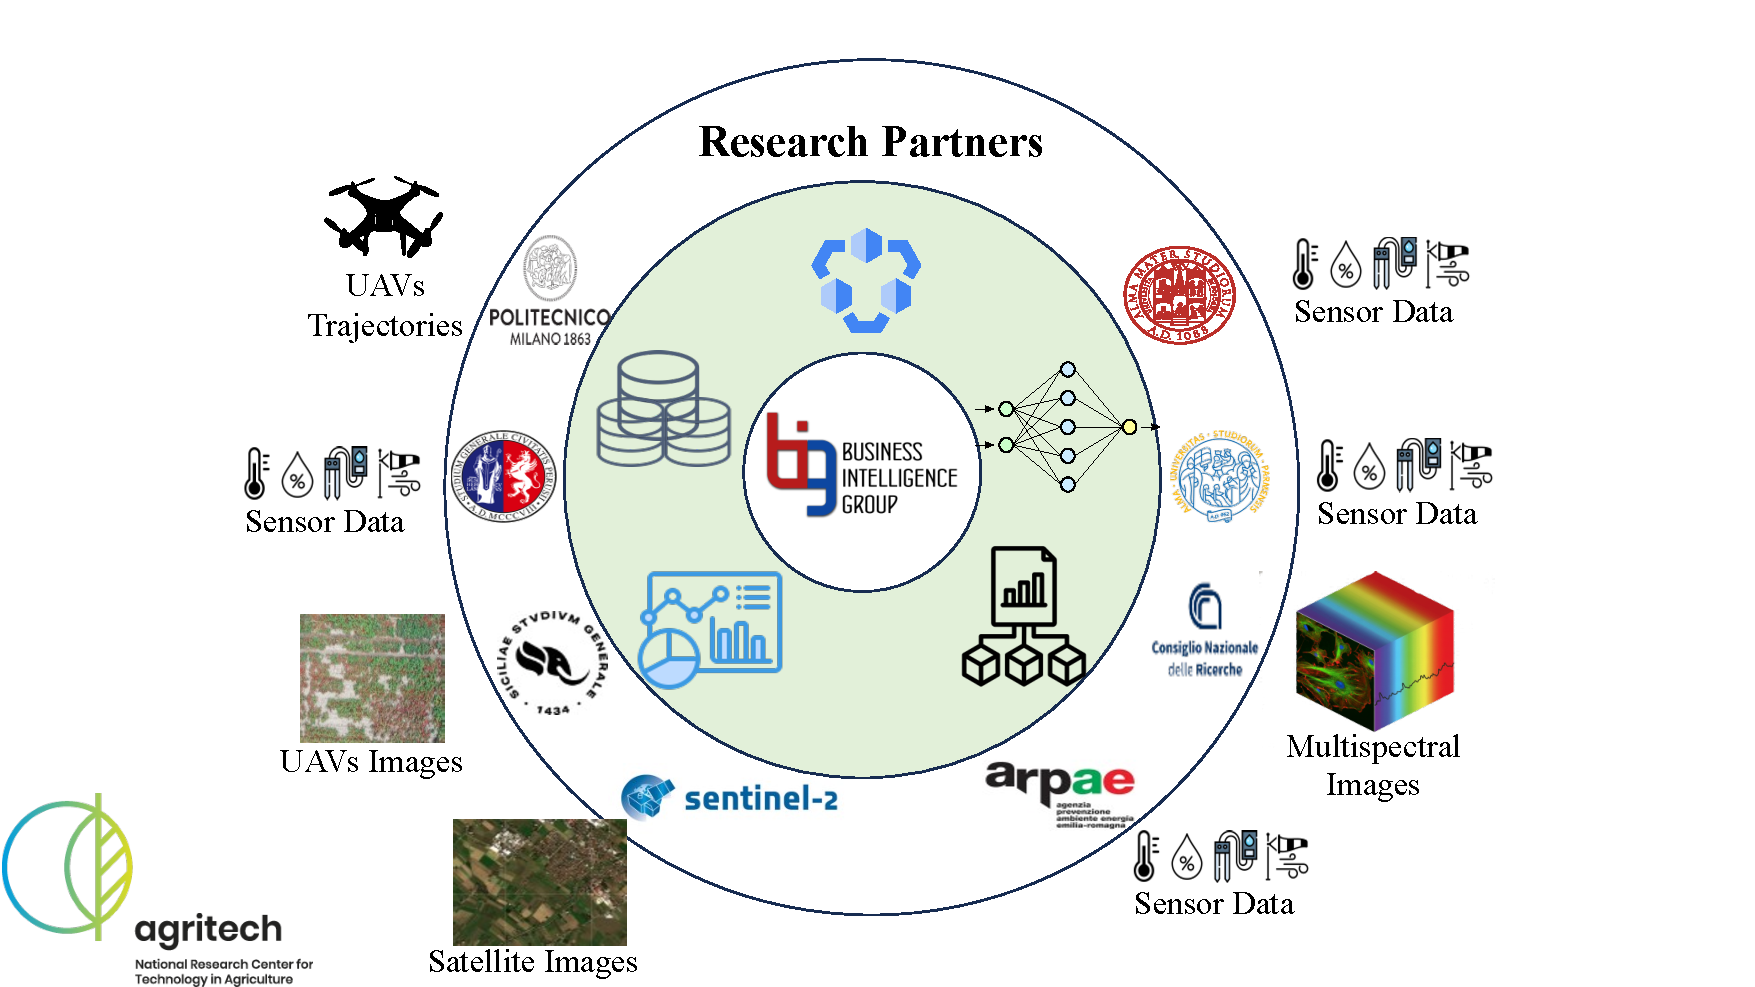
\includegraphics[scale=0.5]{parts/architectures/images/agritech_arch.pdf}
    \caption{Conceptual representations of the nature of the research partners' data.}
    \label{fig:agritech_plat}
\end{figure}

\subsection{Terminology Analysis}

Requirements elicited directly from six partners, however numerous, cannot be assumed to cover the concepts recurring across the precision agriculture domain at large; a platform designed only around them would risk being an accurate model of these six projects rather than of the domain they belong to. To mitigate this risk, the requirements above were cross-checked against an independent analysis of domain terminology, obtained by scraping the accepted papers of the last four editions (2020--2023) of the European Conference on Precision Agriculture (ECPA), and ranking the 1300 most frequent terms out of the 3000 extracted.

This analysis served two purposes. First, it confirmed the centrality of the same data-oriented characteristics identified through the partner interviews: among the ten most frequent terms in the corpus, \emph{sensor}, \emph{data}, \emph{multispectral}, and \emph{image} directly denote the variety of data types just discussed, while \emph{management} and \emph{machine learning} point to the processing and analytics needs the platform is expected to support. Second, and more directly relevant to the schema presented in \Cref{sec:dataplat-refarch}, it distinguished terms denoting real-world entities or measurable properties worth representing explicitly in a conceptual schema (e.g., \emph{crop}, a physical entity, and \emph{yield}, a measurable property of a crop) from terms denoting abstract fields, techniques, or research areas (e.g., \emph{precision agriculture} or \emph{machine learning} itself), which a data-oriented conceptual schema is not intended to represent.

Taken together, these two analyses characterize the data this platform is designed to support along four axes -- variety, volume, veracity, and spatio-temporal reference -- and identify a first candidate set of domain concepts worth representing explicitly. The following sections derive from this characterization, in turn, a reference architecture for the platform (\Cref{sec:dataplat-refarch}) and, building on it, a domain-level data model representing these concepts (\Cref{sec:dataplat-datamodel}).

\section{A Reference Architecture for the Data Platform}

This section describes a reference architecture for the AGRITECH data platform, derived from the characterization of the domain's data in \Cref{sec:dataplat-characterization}. The architecture is organized around independent, composable modules, each responsible for one stage of the data life cycle, from ingestion to exploitation. The following sections describes the conceptual model of the platform (\Cref{sec:dataplat-refarch}) and then discuss technical implementations on an on-premises cluster (\Cref{sec:dataplat-implementation}).

\subsection{A conceptual view}
\label{sec:dataplat-refarch}


\begin{figure}[htbp]
    \centering
    \makebox[\textwidth][c]{%
        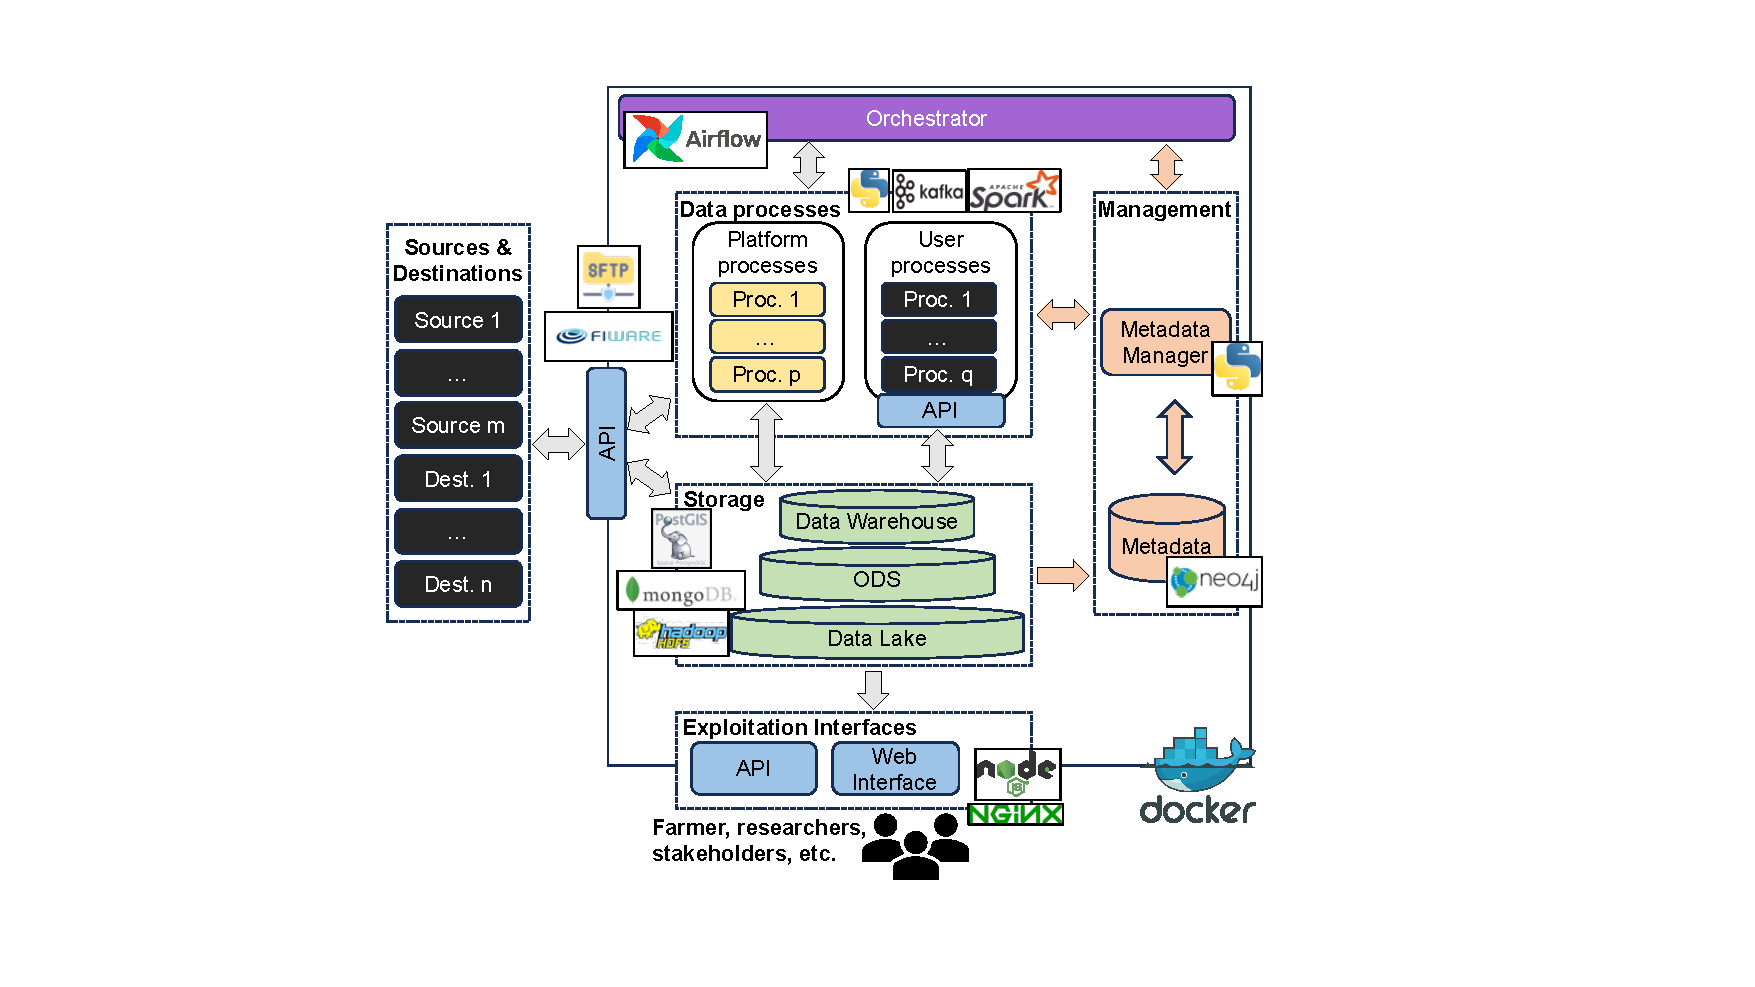
\includegraphics[trim=0pt 45pt 45pt 35pt, clip, width=1.15\textwidth]{parts/architectures/images/agritech_platform.pdf}%
    }
    \caption{A reference data architecture for the AGRITECH data platform, organized around independent, composable modules.}
    \label{fig:agritech_architecture}
\end{figure}

The variety, volume, veracity, and spatio-temporal character of the data identified in \Cref{sec:dataplat-characterization} motivate an architecture organized around independent, composable modules, each responsible for one stage of the data life cycle, from ingestion to exploitation (fig:dataplat-architecture).


\begin{itemize}
    \item \textbf{Ingestion} is responsible for admitting raw data into the platform from heterogeneous sources -- relational or NoSQL databases, files, or third-party APIs such as those providing satellite-derived vegetation indices -- directly reflecting the variety identified above. Three ingestion modes are distinguished: \emph{push} ingestion, in which sources continuously stream data into the platform as it is produced (e.g., a robot updating its GPS trajectory); \emph{pull} ingestion, in which the platform periodically retrieves data from an external source on a fixed or ad-hoc schedule (e.g., downloading a weekly satellite acquisition); and \emph{manual} ingestion, for data collected and uploaded directly by domain experts -- the mode most exposed to the veracity concerns discussed above.
    \item \textbf{Storage} persists both raw and processed data across repositories suited to their variety and volume. Following the standard data-warehousing distinction, the architecture separates \emph{operational} data, addressing the immediate, short-term needs of a process (e.g., the latest sensor reading), from \emph{strategic} data, supporting longer-term, historical analysis (e.g., multi-year pest trends). A data lake accommodates raw data in its native format, irrespective of structure; databases accommodate data conforming to a specific model (relational, document, or graph); and, where reconciled historical analysis is required, an operational data store or a data warehouse accommodates data integrated across sources.
    \item \textbf{Data processes} transform operational data into knowledge of increasing strategic value, spanning both \emph{streaming} processing, producing results within seconds of data arrival, and \emph{batch} processing, operating over larger collections with a longer completion horizon. This module is discussed further below.
    \item \textbf{Management} oversees the data life cycle through profiling and metadata management, addressing the provenance and quality properties that the veracity concerns identified above make especially relevant.
    \item \textbf{Exploitation} governs how raw data or the knowledge derived from it is consumed by its end users, be they developers, domain experts, or other processes running on the platform. Because these users differ significantly in technical background, the architecture supports multiple fruition endpoints, from programmatic APIs to ready-made web interfaces.
    \item An \textbf{orchestrator} coordinates data and management processes into larger, repeatable pipelines, sequencing dependent tasks and scheduling their recurring execution.
\end{itemize}

The distinction drawn above between platform and user processes deserves closer attention, since it is what allows the platform to remain agnostic to the internal implementation of each partner's application, the same property \Cref{chap:data_oriented_perspective} attributed to a Digital Twin Platform with respect to the Digital Twins it hosts, applied here one level down, to the individual processes it hosts.

\emph{Platform processes} are internal to the platform itself, and are typically responsible for producing or maintaining data of shared value across partners. During the requirements gathering phase, it emerged that some data was used by almost every stakeholder: for instance, externally sourced reference data such as satellite imagery produced by Copernicus\footnote{\url{https://dataspace.copernicus.eu/}}, and weather measurements collected by the Regional Agency for Prevention, Environment and Energy of Emilia-Romagna (ARPAE)\footnote{\url{https://www.arpae.it/it}}. Because they are developed and maintained as part of the platform, platform processes are granted direct, trusted access to its storage layer, and ensure that the resulting data conforms to the platform's representation standards, giving all partners a single representation to consume rather than one each (and avoiding the duplicated storage costs of every partner keeping its own copy). Typical platform processes include \emph{data ingestion} (admitting raw data into the platform), \emph{data cleaning} (correcting errors and inconsistencies in the data), and \emph{data integration} (reconciling data from multiple sources into a single representation).

\emph{User processes}, by contrast, are applications deployed and controlled by individual partners, hosted on the platform but developed independently of it and of one another. Consistently with the modularity and independence expected of a data platform \cite{francia2025process}, user processes are treated as black boxes: rather than being granted direct access to the platform's storage, they interact with it exclusively through well-defined APIs. This has a double effect: a partner is free to implement, modify, or replace their own processes without affecting the platform or any other partner's activity, while the platform, in turn, does not need to know how a given user process is implemented internally, only that the data it consumes and produces through these shared interfaces conforms to the same representation standards platform processes are held to. User processes typically implement application-specific pipelines, collecting and transforming the data a given application requires; the same API layer that isolates them from the platform's internals also ensures that the data they produce can, in turn, be consumed by other partners' applications, and vice versa.
-
This separation between a small set of trusted platform processes and an open-ended, partner-defined set of user processes is what allows the platform to scale to a growing and evolving set of partners and applications: what must remain uniform is not the software each process runs, but the representation of the data it exchanges with the platform, discussed next in \Cref{sec:dataplat-datamodel}.

\subsection{Technological Stack}
\label{sec:dataplat-implementation}

The modules identified in \Cref{sec:dataplat-refarch} were implemented on an on-premises cluster, containerized through Docker\footnote{\url{https://www.docker.com/}} in Swarm mode, a choice motivated by cost, long-term availability beyond the project's own duration, and the modularity and fault tolerance a containerized, orchestrated infrastructure affords over a bare-metal deployment. The remainder of this section maps each module of the reference architecture onto the specific technology used to implement it.

\emph{Ingestion} is implemented around FIWARE\footnote{\url{https://www.fiware.org}} and, specifically, its Orion Context Broker, which exposes the NGSI-LD API as the platform's single entry point for context data. Real-world objects are represented as entities conforming to Smart Data Models, each required to carry, at minimum, an identifier, a type, a human-readable name, and the identifier of the owning partner; representative entity types instantiated for AGRITECH include \texttt{Device}, \texttt{AgriFarm}, \texttt{AgriParcel}, \texttt{AgriTree}, \texttt{Camera}, and \texttt{Task}. The three ingestion modes distinguished in \Cref{sec:dataplat-refarch} map directly onto this implementation: push ingestion is realized through Orion's creation and update APIs, pull ingestion through internal processes retrieving data on a schedule, and manual ingestion through SFTP file transfer for partners uploading data directly.

\emph{Storage} is realized as a data lake combining HDFS \cite{white2012hadoop}, holding raw, high-volume data such as satellite archives and robot mission logs, with MongoDB, holding the semi-structured, NGSI-LD-conformant entities produced by the ingestion layer together with their history. The two repositories accordingly reflect the operational/strategic distinction of \Cref{sec:dataplat-refarch}: HDFS as the substrate for large-scale batch processing, MongoDB as the up-to-date, queryable view of the platform's entities.

\emph{Data processes} are supported through Apache Kafka\footnote{\url{https://kafka.apache.org/}} \cite{shapira2021kafka} for streaming and Apache Spark\footnote{\url{https://spark.apache.org/}} \cite{chambers2018spark} for batch workloads. Platform processes exploit this combination in different ways: recurring platform processes retrieve and reconcile externally sourced data, such as ARPAE's weather archives or Copernicus Sentinel-2 imagery, storing the raw archives in HDFS and the resulting SDM-conformant entities in MongoDB; a further platform process historicizes every entity created or updated in Orion by subscribing to the corresponding events, publishing them as a Kafka stream, and persisting them to MongoDB, partitioned by owning partner.

The \emph{orchestrator} is implemented with Apache Airflow,\footnote{\url{https://airflow.apache.org/}} adopted in place of the originally considered Oozie for its Python-based workflow definitions and its web-based monitoring interface, both directly relevant to a platform whose processes are, in large part, contributed and maintained by external partners rather than by the platform's own developers.

Finally, \emph{exploitation} is realized through a web application, served by Nginx\footnote{\url{https://www.nginx.com/}} with a Node.js\footnote{\url{https://nodejs.org/}} backend, centred on an interactive map that renders georeferenced entities by type and exposes their attribute history, alongside a hierarchical view for navigating the platform's entities by owner and type. Programmatic access is provided through APIs specified according to the OpenAPI standard, ensuring that the same representation standards enforced at the level of ingestion and storage extend to how the platform's data is ultimately consumed.

\section{Towards a Domain-Level Data Model}
\label{sec:dataplat-datamodel}

The reference architecture presented in \Cref{sec:dataplat-refarch} standardizes how data is acquired, stored, and made available across the platform's modules, irrespective of what that data represents. As discussed in \Cref{chap:data_oriented_perspective}, however, standardizing this infrastructural layer does not by itself guarantee that the data flowing through it is represented consistently, or that its meaning is preserved as it moves from one partner's application to another's. This section addresses that complementary concern: how the entities relevant to the AGRITECH domain should themselves be represented, so that partners' data can be integrated rather than merely co-located.

\subsection{FIWARE Smart Data Models}

The terminology analysis in \Cref{sec:dataplat-characterization} identifies \emph{what} concepts a shared representation of the domain should cover, but not \emph{how} such concepts should be digitally modelled for effective transmission and storage; neither the literature nor domain dictionaries such as AGROVOC\footnote{\url{https://www.fao.org/agrovoc/}} address this second question. A natural starting point is the FIWARE foundation, which supports the sharing of information across several sectors, including precision agriculture, sensing, and smart cities.\footnote{\url{https://www.fiware.org}} Within FIWARE, real-world objects -- a farm, a parcel, a sensor -- are mapped into digital entities described by \emph{Smart Data Models} (SDM), each composed of a schema defining the entity's attributes and their types, a human-readable specification, and example payloads. Smart Data Models are grouped into subjects belonging to one or more domains, where a domain corresponds to an industrial sector; they are public, free to use, modify, and share, and are explicitly intended as blueprints for real-world applications.

Despite this, adopting Smart Data Models directly, as a shared representation for the platform, would not resolve the fragmentation this chapter is concerned with. Smart Data Models present four limitations in this respect. First, they are designed to be application- and transmission-oriented, which limits the extent to which the data they describe can be extended and integrated into higher-level knowledge. Second, they provide no unified interface for accessing and manipulating the data they describe, so that a data lake populated directly with SDM-conformant entities risks becoming, in practice, a data swamp in which the necessary data is difficult to locate even when present. Third, they exhibit intra- and inter-domain inconsistencies and redundancy: the same real-world concept can exist in different domains with different semantics or attributes -- a greenhouse, for instance, is modelled as a \texttt{Building} in the Smart City domain but as a first-class \texttt{AgriGreenhouse} in the Precision Agriculture domain\footnote{\url{https://smart-data-models.github.io/dataModel.Building/Building/} and \url{https://smart-data-models.github.io/dataModel.Agrifood/AgriGreenhouse/}} -- and the same concept can be modelled in more than one way even within the same domain, as when a sensor measurement is represented directly as an attribute of a \texttt{Device} in one case and as a first-class \texttt{DeviceMeasurement} in another.\footnote{\url{https://smart-data-models.github.io/dataModel.Device/Device/} and \url{https://smart-data-models.github.io/dataModel.Device/DeviceMeasurement/}} Fourth, distinct notions are sometimes aggregated within a single concept -- for instance, a sensor and its measurement within the same \texttt{Device} -- to keep the resulting payloads compact and efficient to transmit (e.g., over MQTT); the same tendency to aggregate distinct notions for the sake of compactness has been reported in ontologies developed for the agricultural domain more generally \cite{jonquet2018agroportal,hu2011agont}.

These limitations motivate defining an integrated, domain-level conceptual schema, rather than adopting Smart Data Models as they stand: the goal is to map the entities exposed at the level of individual sources and applications onto a restricted set of higher-level concepts, atop which analytics can be carried out uniformly across partners. As a first step in this direction, the entities and attributes identified across the six partners' projects were matched, where possible, against existing Smart Data Models (\Cref{tab:sdm-mapping}). This mapping exercise showed that (i) not every entity has a ready SDM counterpart, so that new models must sometimes be created or existing ones extended; (ii) more than one SDM representation is occasionally available for the same entity, requiring an explicit choice between them; and (iii), most importantly, that the entities involved could be generalized into a small number of recurring notions -- agents, measurements, tasks, and environments -- which the domain-level conceptual schema presented next takes as its starting point.

\begin{table}[h!]
\centering
\caption{Mapping selected domain concepts to FIWARE Smart Data Models.}
\label{tab:sdm-mapping}
\begin{tabular}{lll}
\toprule
\textbf{Term} & \textbf{FIWARE SDM} & \textbf{Standardized Concept} \\
\midrule
Robot, Weather station & Device & Agent \\
AI process & -- & Agent \\
Temperature, Humidity & Device, DeviceMeasurement & Measurement \\
Weeding, Monitoring & -- & Task \\
Emilia Romagna & -- & Environment \\
Parcel & AgriParcel & Environment \\
Farm & AgriFarm & Environment \\
\bottomrule
\end{tabular}
\end{table}

\subsection{A Domain-Level Conceptual Schema}

The terminology analysis in \Cref{sec:dataplat-characterization} identified candidate domain concepts but not the relationships among them, nor a criterion for deciding which concepts belong in a shared schema and which are better left to individual applications. The conceptual schema addresses both questions, organizing the identified concepts into four zones (\Cref{fig:dataplat-schema}).

\begin{figure}[h!]
    \centering
    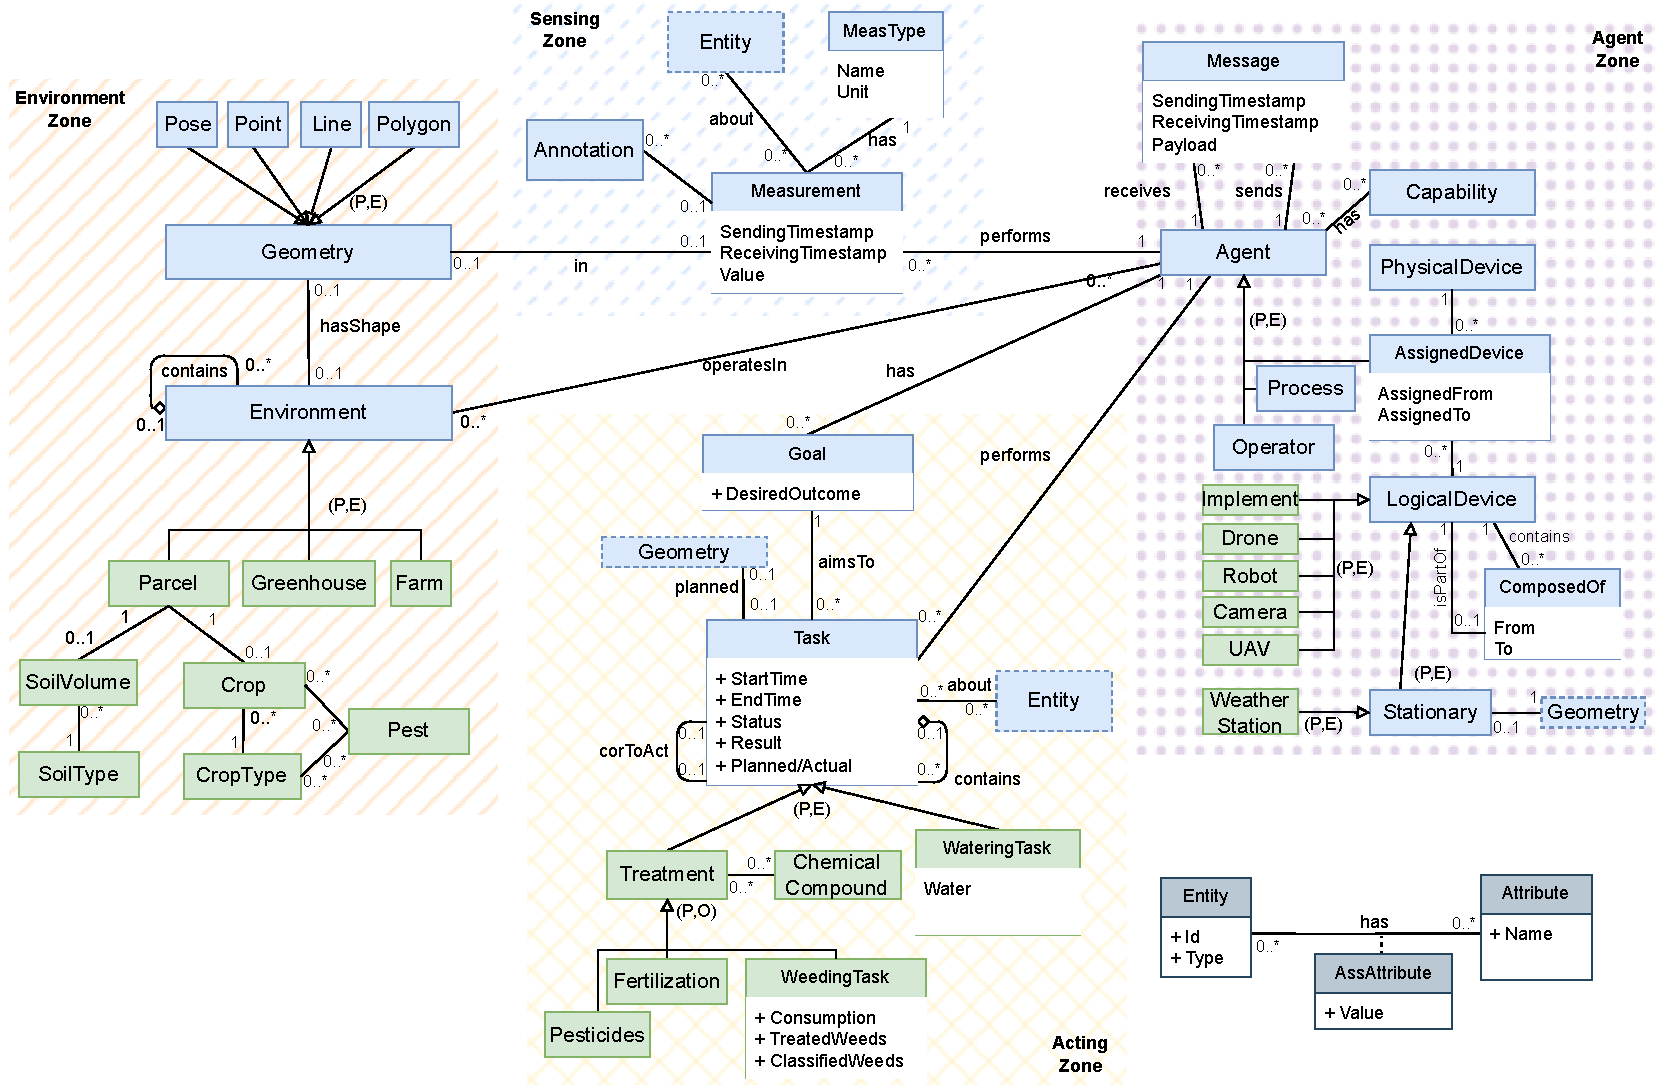
\includegraphics[scale=0.5]{parts/architectures/images/agritech_dm.pdf}
    \caption{The proposed AGRITECH domain-level conceptual schema, organized into four zones: agent, environment, sensing, and acting.}
    \label{fig:dataplat-schema}
\end{figure}

The data model  schematizes the main components of Digital Twins and their conceptual organization as much as its hierarchical structure. The \emph{agent} zone represents the master data of entities that sense and act within an environment to pursue a goal: an \texttt{Operator} is a human agent (e.g., a farmer), a \texttt{Process} is an ICT agent with no physical counterpart (e.g., an AI vision system), and a \texttt{LogicalDevice} represents the role played, at a given time, by some \texttt{PhysicalDevice}: such a distinction allows, for instance, a faulty physical sensor to be replaced without altering the logical identity of the measurement point it realizes. The \emph{environment} zone represents the hierarchical, georeferenced areas in which agents operate (e.g., a farm composed of parcels). The \emph{sensing} zone represents the history of data sensed by an agent, as \texttt{Measurement}s characterized by a type, a precision, and an accuracy, and optionally annotated (e.g., a bounding box marking a detected weed within an image). The \emph{acting} zone represents the history of actions an agent undertakes, as hierarchically composed \texttt{Task}s with associated space and time dimensions, and both a planned and an executed form.

Concepts in each zone are further distinguished as either \emph{domain-agnostic} (in blue in \Cref{fig:dataplat-schema}), when generic enough to fall outside precision agriculture altogether and to be assimilated directly to the notion of a Digital Twin itself, as components recurring in a Digital Twin regardless of its domain (e.g., \texttt{Agent}, \texttt{Task}, \texttt{Measurement}), or \emph{domain-specific} (in green in \Cref{fig:dataplat-schema}), when specialized to a specific domain; in this case, the agritech setting (e.g., \texttt{Crop}, \texttt{Parcel}, \texttt{Farm} as specializations of \texttt{Environment}, or \texttt{Robot} and \texttt{WeatherStation} as specializations of \texttt{LogicalDevice}). This distinction is what makes the schema extensible to concepts not yet identified: a new domain-specific concept can be introduced as a specialization of an existing domain-agnostic one without revising the schema itself.
Similarly, the domain-agnostic concepts are intended to be reusable across domains, so that a new domain-specific concept can be introduced as a specialization of an existing domain-agnostic while still having some common ground with other domains, and without requiring a new schema to be defined from scratch.



%%%%%%%%%%%%%%%%%%%%%%%%%%%

\chapter{STGraph - A Multistore system for Digital Twins}
\label{chap:stgraph}
\label{chap:datamodel-dt}


\Cref{chap:dataplat} proposes a generic data architecture of an individual Digital Twin, first through the reference architecture and requirements analysis of \Cref{sec:dataplat-refarch,sec:dataplat-characterization}, and then through the domain-level conceptual schema of \Cref{sec:dataplat-datamodel}, which represents the AGRITECH domain in terms of agents, environments, measurements, and tasks. That architecture, however, focuses mainly on system standardization and the conceptual logical organization of data in it through the proposal of a software infrastructure necessary to sustain the data pipelines collecting and integrating data and the application-level functionality of a hypothetical Digital Twin, but does not address the problem of the conceptual representation of such data in terms of the data model needed to efficiently integrate and query the data flowing through the platform, nor does it address the physical data management systems needed to implement such a model.

A first, natural candidate is to implement the conceptual, object-oriented schema of \Cref{sec:dataplat-datamodel} through a relational model and DBMS, as it is standard practice for structured, schema-first data. However, while a relational DBMS are quite efficient in storing and querying long series of data, such as the ones produced by sensors attached to the physical entity in a Digital Twin, they expose two difficulties that are at the same time characteristic of precision agriculture and , more generally, Digital Twin data. The first concerns the dynamic relationships among entities. Several of the relationships identified in \Cref{sec:dataplat-datamodel}, such as which physical device realizes which logical role, which sector a device is currently assigned to, which thesis is being tested on which sector, do not hold once and for all, but only for a bounded interval of time, and are expected to change repeatedly over a Digital Twin's operational life. Being many-to-many relationships, representing them in a relational model requires dedicated association tables carrying explicit validity intervals, and reconstructing even a moderately complex configuration (i.e. which devices were assigned to which sector, and when) requires joining across several of such tables; as a consequence query performances tend to degrate and maintaining consistence through such table is an extremey time consuming and error-prone task. Furthermore, as these dynamic relationships accumulate, the resulting schema increasingly resembles a network of interconnected entities in which the connections themselves, and their evolution over time, matter as much as the entities they relate: a setting for which the relational model, built around fixed tables and predetermined join paths, is not a natural fit, and towards which graph data models are more directly suited. The second difficulty concerns extensibility: a relational schema fixes, in advance, the set of tables and relationships a schema can represent, so that supporting a new kind of entity, or a new kind of relationship between existing entities, as new functionality is added to the platform, generally requires revising the schema itself -- the same rigidity \Cref{chap:digital_twins,chap:data_oriented_perspective} identified as an obstacle to standardization across evolving, heterogeneous Digital Twin deployments.

These two difficulties motivate considering a graph data model for the entities characterized in \Cref{sec:dataplat-datamodel} and their relationships. Graphs represent entities and relationships uniformly, as nodes and edges, without committing in advance to a fixed schema, so that new entity or relationship types can be introduced without revising an existing structure; and they can represent the temporal evolution of a relationship as a property of the edge realizing it, rather than as an artifact of the physical schema. At the same time, Digital Twin data is not only about the graph of relatively stable entities: it also includes the high-volume, high-frequency time-series data produced by sensors and devices, identified in \Cref{sec:dataplat-characterization} as a defining characteristic of the domain. A graph model well suited to representing entities and their evolving relationships is not, by itself, designed to efficiently store and query such high-frequency time-series; conversely, a data management system optimized for time-series is not designed to represent the rich, evolving topology connecting them to the entities that produce them. This coexistence of graph and time-series data motivates the data model, and the physical system necessary to implement it, presented in this chapter.

The following section presents STGraph, a data model, and its own multistore implementation, that represents slowly evolving entities as a spatio-temporal property graph while managing high-volume, georeferenced time-series through a dedicated time-series store, connecting the two through a shared, efficient representation.
%
Such system has been evaluated in hybrid graph-time-series workloads typical of Digital Twins applications, showing that it can reduce storage footprint and improve ingestion and query performance with respect to temporal graph and multistore baselines.


\section{Introduction}

\label{sec:stgraph_paper}
The unprecedented volume and variety of data generated by the Internet of Things and the rapid adoption of digital twin technologies pose new challenges to data management systems.
On the one hand, modern applications require flexible data models capable of representing evolving spatio-temporal topologies of schemaless entities.
On the other hand, they require optimized mechanisms for ingesting, storing, and querying massive collections of geo-referenced time-series generated by these connected entities.
Relational systems provide mature query capabilities but lack the flexibility required to manage schemaless data.
Graph systems offer expressive representations of complex relationships; however, they are generally not designed to efficiently handle high-volume time-series data.
In this paper, we present \ourapproach, a multistore for spatio-temporal property graphs that combines the expressiveness of spatio-temporal property graph data models with the efficiency required for time-series.
\ourapproach exposes high-volume time-series events as logical graph nodes while persisting and processing them in a dedicated store.
\ourapproach connects graph entities and time-series events through virtual edges, avoids materializing one graph edge per event, and pushes event-local operators to the time-series store.
Our evaluation against temporal graph and multistore baselines shows that this design reduces storage footprint and improves ingestion and query performance on graph-time-series workloads.


The availability of new types of data gives rise to new types of analysis and, consequently, poses new challenges in data management.
The widespread deployment of Internet of Things infrastructures and the rapid adoption of digital twin technologies~\cite{DBLP:journals/cacm/SakrBVIAAAABBDV21} have introduced the need for coupling the analysis of long time-series with semantically rich and complex information.

\begin{example}[Healthcare]
The availability of time-series data on vital signs and physical devices (e.g., pacemakers)~\cite{montagna2020real}, as well as on patients' daily behaviors and medical histories (e.g., treatments, medical conditions), allows physicians to analyze complex cause-and-effect relationships and compare data from multiple patients with similar characteristics.
\end{example}

\begin{example}[Precision agriculture]
Fleets of robots operating in agricultural fields (that belong to a farm, have different crop types, and are managed by different farmers) generate hundreds of georeferenced events per minute~\cite{emmi2023exploiting}.
Integrating these heterogeneous data streams with master data of farms, fields, and crops allow to better understand temporal and spatial activities, transforming precision agriculture systems from mere monitoring tools into proactive, context-aware decision support frameworks.
\end{example}

The examples above pose several data management challenges~\cite{DBLP:journals/sigmod/Tian22}.
The schema-less nature of IoT data requires the adoption of a data model that is both \emph{flexible} and \emph{expressive} to enable the correlation of data that is heterogeneous in nature. 
The ever-changing nature of the data and their spatial characterization require \emph{spatio-temporal query capabilities} and an \emph{efficient versioning} of historical data. 
%(e.g., to know which robots have operated in a field, and when).
The massive volume of long and high-frequency \emph{time-series} requires the ability to \emph{efficiently manage their querying and ingestion}.
The rate at which time-series events are generated can be orders of magnitude greater than that of other types of information, and this crucial factor calls for specialized solutions. 

Relational Database Management Systems (DBMSs) provide a mature and expressive query model supported by decades of optimization research.
However, their schema-first design is less suitable for applications with rapidly evolving, heterogeneous, or semi-structured data, as in IoT and digital twin scenarios.
Moreover, although relational systems can store temporal data, they are not designed for high-rate ingestion or analytical processing of massive time-series measurements.
Graph data models offer an attractive alternative, combining expressive traversals with schema-optional flexibility.
They naturally capture complex relationships among entities and support evolving schemas, making them well suited for semantically rich, interconnected, temporal, and spatial data.
Nevertheless, graph DBMSs are not optimized for dense event streams, where workloads are dominated by sequential writes, time-based filtering, and aggregation.
Conversely, time-series DBMSs support high-throughput ingestion and efficient time-oriented queries over large event collections.
Their data model and query capabilities, however, remain specialized for time-series workloads and lack the expressive power needed to model complex semantic relationships among heterogeneous entities.

These complementary strengths and limitations motivate a multistore architecture~\cite{DBLP:journals/csur/BestaGPFPBAH24,DBLP:journals/sigmod/BonifatiOTVYZ24}, where each database system is responsible for the workload it is designed to support.
However, simply placing a graph DBMS next to a time-series DBMS is not sufficient: applications still need a single graph abstraction, graph traversals must cross the store boundary without materializing one edge per event, and selections, projections, and aggregations over events must be pushed to the time-series store without changing query semantics.
The novelty of \ourapproach lies in this cross-store graph/time-series boundary: time-series events remain logical graph nodes and are reached through virtual graph edges, while their physical storage, ingestion, and event-local computation are delegated to TS.

\begin{figure}[t]
\centering
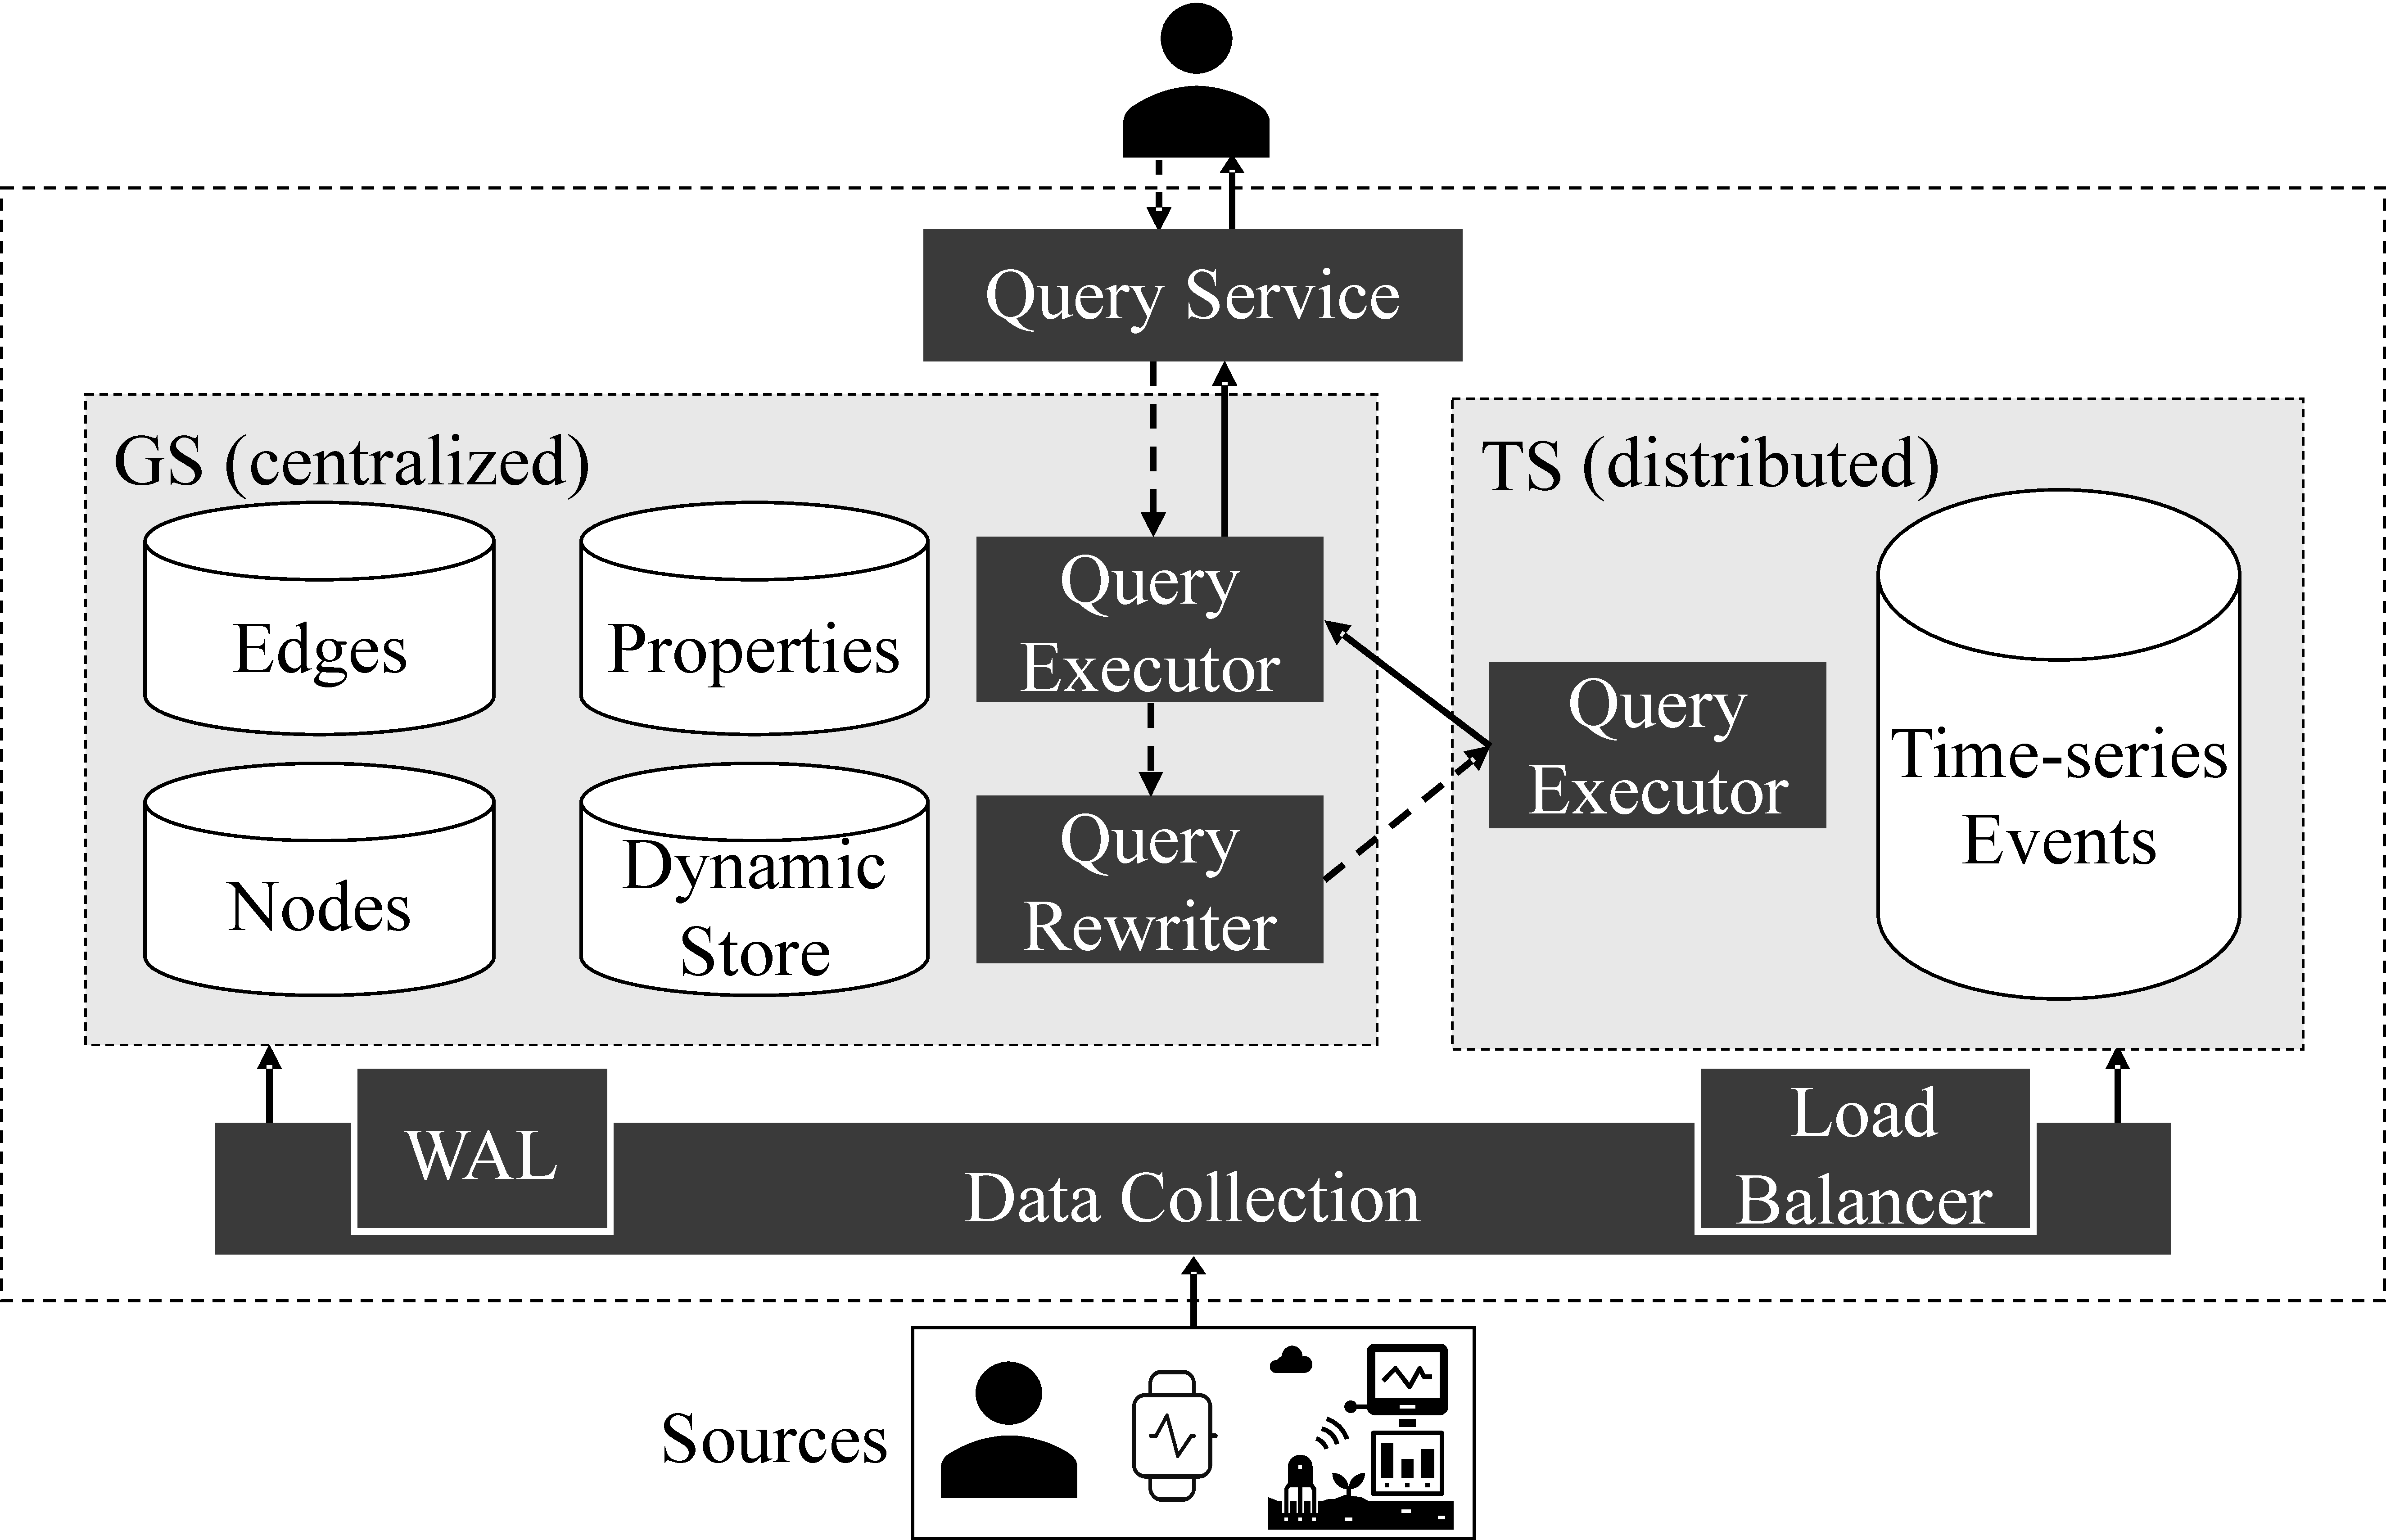
\includegraphics[scale=0.10]{parts/architectures/images/architecture.pdf}
\caption{\ourapproach: straight arrows represent data flows, while dashed arrows represent query-rewriting flows.}
\label{fig:overview}
\end{figure}

\paragraph{Overview and contributions}
We introduce \ourapproach (\Cref{fig:overview}), a multistore for managing spatio-temporal property graphs containing both slowly evolving entities and high-volume geo-referenced time-series events.
From the logical perspective, all data are queried as nodes, edges, and properties.
This choice is taken since graphs natively support interconnected, schemaless and evolving data; evolution is modeled by versioning graph entities with temporal validity and by supporting temporal traversal.
Physically, \ourapproach separates the workload between a Graph Store (GS), which stores materialized graph entities and relationships, and a Time-series Store (TS), which stores events.
The key design point is that events are exposed as graph nodes but are not materialized in GS: they are reached through virtual edges generated during traversal, and event-local predicates, projections, and aggregations are compiled into TS requests.
%, providing a unified abstraction that combines expressive graph querying with scalable time-series management.
At the bottom of \Cref{fig:overview}, data sources upsert data through the ``Data Collection'' service, which is responsible for dispatching the data to either GS or TS.
Uploading data to TS does not require interaction with GS (and vice versa), enabling fully independent management of static/dynamic data.
At the top of \Cref{fig:overview}, users query the spatio-temporal property graph through the ``Query Service'', which interprets the incoming query and transforms it into a query plan that is forwarded to the ``(GS)  Query Executor.''
During graph traversal, if the query requires data from TS, the ``(GS)  Query Executor'' invokes the ``Query Rewriter,'' which translates and pushes the query down to the ``(TS) Query Executor.''
Finally, results are shuffled and aggregated by the ``(GS)  Query Executor.''
%,'' which returns them to the ``Query Service.''

The contributions of \ourapproach are the following.
\begin{enumerate}[label=(\roman*)]
    \item A spatio-temporal property graph abstraction in which time-series events are treated as logical graph nodes, while their physical representation remains in a time-series store.
    \item A multistore storage layout that connects GS and TS through shared identifiers and virtual edges, avoiding the materialization of one graph edge per event while preserving graph traversal semantics.
    \item Cross-store query optimization that pushes event-local selections, projections, and decomposable aggregations to TS and combines their results in GS.
    \item An experimental evaluation against (temporal) graph and multimodel baselines, showing lower storage footprint and faster ingestion/query execution on graph-time-series workloads.
\end{enumerate}

The paper is organized as follows.
\Cref{sec:related} compares \ourapproach with the state-of-the-art contributions.
\Cref{sec:formal} defines the spatio-temporal property graph.
\Cref{sec:stgraph} introduces the multistore storage layout while
\Cref{sec:query} describes the query execution and optimization.
\Cref{sec:exp} extensively tests \ourapproach.
\Cref{sec:conclusion} draws the conclusion and future research directions.

\section{Related Work}\label{sec:related}
The management of schemaless, evolving, and time-series data has received significant attention.
Existing systems can be grouped into single-model, which optimize either time-series or graph workloads, and multimodel/multistore, which combine multiple models but do not provide native cross-store graph traversal over time-series.

In summary, prior systems provide either efficient time-series storage without graph-native traversal, temporal graph management without scalable event ingestion, or multimodel integration through middleware.
\ourapproach does not expose time-series data merely as external attributes, views, or relational extensions, but it makes time-series events logical graph nodes, linking them to GS nodes through virtual edges, and pushes event-local operators down to TS during traversal between GS and TS.
\subsection{Single model solutions}

\subsubsection{Time-series}
Time-series DBMSs have gained popularity with the rise of IoT and digital twins applications in recent years~\cite{DBLP:journals/tkde/JensenPT17}.
Time-series DBMSs usually rely on indexes, such as Log-Structured Merge Trees (LSM-Trees)~\cite{DBLP:journals/acta/ONeilCGO96}, which buffer write operations in memory and flush them to disk in batches, drastically reducing the number of disk accesses and thus achieving exceptional ingestion performance.
%Compaction policies are then progressively performed to organize data as it is flushed to disk.
InfluxDB\footnote{https://www.influxdata.com/} is among the most widely adopted time-series DBMSs.
InfluxDB's primary focus lies in the efficient storage and retrieval of high-volume time-series, rather than in modeling the underlying entities.
Several solutions have been proposed in the literature to address time-series data, such as Apache IoTDB~\cite{DBLP:journals/pvldb/0018HQ00MFZ0ZKJ20}, AsterixDB~\cite{DBLP:journals/pvldb/AlsubaieeAABBBCCCFGGHKLLOOPTVWW14}, and Gorilla~\cite{DBLP:journals/pvldb/PelkonenFCHMTV15}.
Within these, AsterixDB is a shared-nothing distributed big data management system designed to efficiently manage large volumes of semi-structured data.
It adopts a flexible data model based on nested, schema-less records and organizes information into datasets stored on LSM-tree-based storage structures.
%Each dataset is indexed and hash-partitioned across the nodes of the cluster. % using a primary key.

Overall, time-series DBMSs provide the physical properties required by high-rate event workloads, but they do not expose events as part of a rich graph topology and therefore cannot directly express graph traversals over the entities that produce those events.

\subsubsection{(Temporal) Graph}
Graph DBMSs are well-suited for managing highly interconnected environments.
%Their data layout often relies on an index-free adjacency principle that enables efficient relationship navigation via direct neighbor access, making path traversal operations highly efficient.
Neo4J~\cite{Neo4J2025} employs a storage layout built on an index-free adjacency data structure.
However, it does not offer native support for temporal data and its performance tends to degrade when time-series events are represented as ordinary graph nodes and edges.
Recent works have exploited LSM-trees for scalable management~\cite{DBLP:journals/pacmmod/MoLWL25,DBLP:journals/corr/abs-2411-06392}.
However, they are not temporal graphs since they lack versioning.

Debrouvier et al.~\cite{DBLP:journals/vldb/DebrouvierPPSV21} provide a classification of temporal graphs with respect to how temporal information is managed and queried.
%and temporal query semantics:
\textit{Duration-labeled}~\cite{DBLP:journals/tkde/WuCKHHW16}: each edge is annotated with a duration of the relationship.
% between two nodes. 
%At a certain time, a node is considered valid if it participates in at least one edge that is valid at that time.
%This approach is mainly used for scheduling problems, where some shortest path has to be computed and they entail a fixed time granularity.
\textit{Interval-labeled}~\cite{DBLP:journals/vldb/DebrouvierPPSV21}: each node/edge is annotated with a validity interval.
%these temporal graphs could be seen as a generalization of duration-labeled graphs, in which each node/edge is annotated with a validity interval.
This solution allows for a non-fixed time granularity and additional temporal query semantics at the cost of a storage overhead.
\textit{Snapshot-based}~\cite{DBLP:journals/tkde/SemertzidisP19,DBLP:journals/tos/MiaoHLWYZPCC15,DBLP:journals/tlsdkcs/Massri0PM23,DBLP:journals/pvldb/HouZWLJWD24}: represent the graph as a sequence of discrete snapshots at different interval times.
%
Hybrid solutions, such as Copy+Log~\cite{DBLP:journals/tos/MiaoHLWYZPCC15}, $\delta$-Copy+Log~\cite{DBLP:journals/tlsdkcs/Massri0PM23}, and Anchor+Delta~\cite{DBLP:journals/pvldb/HouZWLJWD24}, have been introduced to optimize delta updates of snapshots.
%
Despite each approach optimizes its predecessor through redundancy reduction, snapshot-based representations entail significant storage overhead, which limits their scalability when managing highly dynamic data and large-scale graphs. 

To the best of our knowledge, AeonG~\cite{DBLP:journals/pvldb/HouZWLJWD24} is the state of the art for temporal graphs.
Its Anchor+Delta design balances storage efficiency and query performance by reducing redundant data and limiting read amplification during temporal queries.
% Additionally, the evaluation of AeonG is restricted to relatively small datasets, focusing primarily on small-range and point temporal queries.
With respect to T-GQL~\cite{DBLP:journals/vldb/DebrouvierPPSV21}, Clock-G~\cite{DBLP:journals/tlsdkcs/Massri0PM23}, and AeonG~\cite{DBLP:journals/pvldb/HouZWLJWD24}, \ourapproach follows interval-labeled temporal semantics but targets a different systems problem: time-series events remain queryable as graph nodes while being stored and processed in a dedicated TS backend.

\subsection{Multimodel and multistore solutions}
\subsubsection{Multimodel}
Graphix~\cite{DBLP:conf/icde/Galvizo024} extends AsterixDB with interconnected views over time-series data.
Nonetheless, Graphix does not natively support temporal graphs and relies on logical views over AsterixDB records rather than on a graph/time-series storage split with virtual traversal edges.
Hygraph~\cite{DBLP:conf/edbt/Ammar0BR25} integrates graphs and time-series in a hybrid in-memory data structure.
Time-series are represented as node properties; however, this prevents the possibility to link and assign properties to single events.% and introduces operators to create graph overlays from time-series data.
Being in-memory, Hygraph provides fast graph ingestion but is limited by main-memory capacity and not persistent.% multistore execution.


\subsubsection{Multistore}
AGTS is a multistore solution based on PostgreSQL~\cite{DBLP:conf/sigmod/StonebrakerR86} extended with Apache AGE\footnote{https://age.apache.org/}, TimescaleDB\footnote{https://www.tigerdata.com/}, and PostGIS\footnote{https://postgis.net/}.
PostGIS enhances PostgreSQL with spatial capabilities, TimescaleDB introduces efficient time-series data management via hypertables, and Apache AGE introduces graph capabilities through a hybrid query language (SQL functions that parse Cypher syntax).
Graph data is implemented as logical abstractions on top of PostgreSQL's relational storage model, where each node and edge label is mapped to a corresponding relational table (graph traversals are executed through relational operators rather than native graph-processing mechanisms).

\section{Spatio-temporal property graph}\label{sec:formal}

A spatio-temporal property graph extends the traditional property graph, incorporating both temporal and spatial dimensions.

\begin{definition}[Property graph]\label{def:pg}
A property graph is a tuple:
$G = (N, E, L, P, \ell, \rho)$
where: $N$ is the set of nodes, $E \subseteq N \times N$ is the set of directed edges, $L$ is the set of labels, $P$ is the set of key-value properties, $\ell: N \cup E \to L$ maps each node/edge to a label, $\rho: N \cup E \to 2^P$ maps each node/edge to a set of key-value properties.
\end{definition}
For the sake of brevity, in the remainder of the paper we will refer to node/edge labels and properties using the dot notation (e.g., $n.name$ for the name property of node $n$ and $n.label$ for the $\ell(n)$).

Given the temporal domain $\mathbb{T}$ and the set of spatial objects $\mathbb{S}$, we extend \Cref{def:pg} to a spatio-temporal property graph.

\begin{definition}[Spatio-temporal property graph]\label{def:stg}
A spatio-temporal property graph $G^{st} = (N, E, L, P, \ell, \rho, \ftemporal)$ extends a property graph $G$, where:
$\ftemporal: N \cup E \cup P \to \mathbb{T}^2$ assigns temporal interval validity $[from, to)$ (with $from < to$) to nodes, edges, and properties, enabling an interval-labeled temporal graph; and
$\prop{location}{x} \in P$ is a property that assigns a spatial object $x \in \mathbb{S}$ to nodes and edges.
\end{definition}

Note that (i) node/edge validity must include the validity of its properties, and properties with the same key belonging to same entity cannot have overlapping validity; and (ii) $\texttt{location}$ is a property and not a first-class citizen since nodes/edges can change locations over time (e.g., a person changing the home address).

\begin{figure}[t]
    \centering
    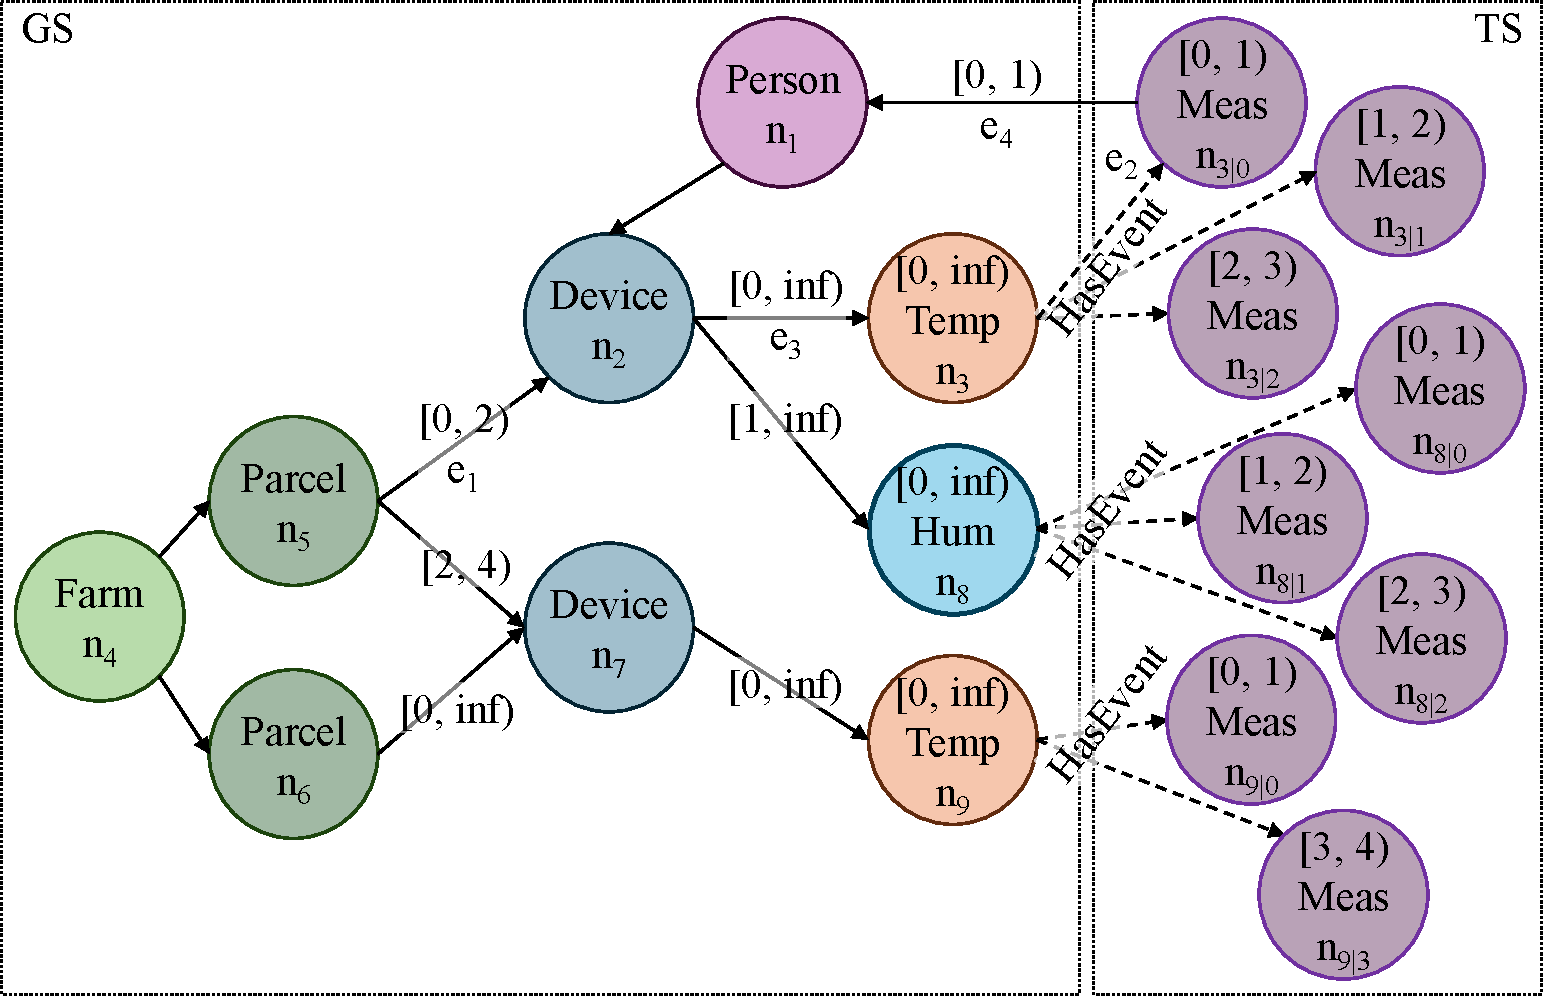
\includegraphics[scale=.32]{parts/architectures/images/example.pdf}
    \caption{Example of a spatio-temporal property graph.
    Different colors represent different node labels. 
    Temporal validity is reported; if omitted, the validity is $(-\inf, \inf)$.
    Node $n_1$ ($``Alice"$, with label \lbl{Person}) is the owner of $n_2$ ($``Device~1"$, \lbl{Device}) (e.g., a weather station) producing two time-series $n_3$ ($``Temp~1"$, \lbl{Temperature}) and $n_8$ ($``Hum~1"$, \lbl{Humidity}).
    $n_4$ ($``Farm~1"$, \lbl{Farm}) is composed of $n_5$ ($``Parcel~1"$, \lbl{Parcel}) and $n_6$ ($``Parcel~2"$, \lbl{Parcel}) that share $n_7$ ($``Device~2"$, \lbl{Device}) producing a time-series $n_9$ ($``Temp~2"$, \lbl{Temperature}).
    $n_5$ also contains $n_2$.
    Edges with label \lbl{HasEvent} are dynamically generated at query time.}
    \label{fig:example}
\end{figure}

\begin{example}
Let $G^{st}$ represent a spatio-temporal property graph modeling \Cref{fig:example}.
The set of nodes $N$ contains $n_2$ (a weather station), $n_5$ (a parcel), and $n_{3|0}$ (a measurement).
The set of edges $E$ contains $e_1 = (n_5, n_2)$ and $e_2 = (n_3, n_{3|0})$.
Examples of labels, properties, and temporal validity are:
\[
\begin{aligned}
n_5.label = \lbl{Parcel}&,\quad e_2.label = \lbl{HasEvent}\\
\rho(n_5) = \{\prop{name}{``Parcel~1"}&,\prop{location}{Polygon(\ldots)}\}\\
\rho(n_{3|0}) = \{\prop{value}{16}&,\prop{unit}{``C"},\prop{location}{Point(\ldots)}\}\\
\ftemporal(n_{3|0}) = [0,1)&,\quad \ftemporal(e_1)= [0,2)
\end{aligned}\]
%\rho(n_2) = \{\prop{name}{``Device~1"}&,\prop{type}{``Weather~Station"}\}\\
\end{example}

\subsection{Operators and query plan}

% We distinguish between the operators necessary to build the spatio-temporal property graph and those used to query it.

% \subsubsection{Versioning the graph}

% Building and versioning the spatio-temporal property graph is based on the following operators.
% \begin{enumerate}
%     \item $\textsf{create}(n)$ (creating a node) adds $n$ to the graph (i.e., $G^{st}.N = G^{st}.N \cup \{n\}$) with a time period $\ftemporal(n)=[from, to)$.
%     Unless otherwise specified, $to = \inf$.
%     \item $\textsf{create}(e)$ (creating an edge) adds $e = (v_1, v_2)$ to the graph (i.e., $G^{st}.E = G^{st}.E \cup \{e\}$) with a time period $\ftemporal(e)=[from_e, to_e)$, where $\ftemporal(e)$ is bounded by the time spans $\ftemporal(v_1)=[from_{v_1}, to_{v_1})$ and $\ftemporal(v_2)=[from_{v_2}, to_{v_2})$.
%     Formally, $from_e \ge max(from_{v_1}, from_{v_2})$ and $to_e \le min(to_{v_1}, to_{v_2})$.
%     Unless otherwise specified, $to_e = \inf$ (i.e., it has no end validity).
%     \item $\textsf{upsert}(x, p)$ (update/add a/to node/edge $x$ with a property $p$) adds $p$ to the graph (i.e., $G^{st}.P = G^{st}.P \cup \{p\}$) with a time period $\ftemporal(p)=[from_p, to_p)$, where $\ftemporal(p)$ is bounded by $\ftemporal(x)=[from_x, to_x)$.
%     Formally, $from_p \ge from_x$ and $to_p \le to_x$.
%     Note that (i) if $x$ already contains a property $p'$ with the same key, $p'.to$ is set to $p.from$; and (ii) adding a property does not update the validity of the node/edge (since its validity could be longer than that of the single property (but the property cannot exceed the validity of the node/edge to which it belongs).
%     \item $\textsf{delete}(x)$ (deleting a node/edge/property) changes its temporal validity from $\ftemporal(x) = [from, to)$ to $\ftemporal(x) = [from, to')$, where $to' < to$.
%     When a node is deleted, all its edges and properties are deleted as well.
%     When an edge is deleted, all its properties are deleted as well.
% \end{enumerate}
% To be valid, a spatio-temporal property graph requires the above temporal constraints to be satisfied, but it does not require any spatial constraint (e.g., a weather station installed in a farm can ``cover'' a surface larger than the farm).

%Creating an element inserts a record with validity $[from,\inf)$ unless a \textit{to} timestamp is provided.
%Deleting an element closes its validity interval by setting its $to$ timestamp.
%Updating a property closes the validity of the previous property record and creates a new property record with the new value and validity.
%Note that these operators do not require materializing full graph snapshots or maintaining separate delta structures.
%For instance, in \Cref{fig:example}, $n_2$ was added to $n_5$ and then removed, resulting in an edge $e$ with temporal validity $\ftemporal(e)=[0, 2)$; no additional graph snapshot is required.

% \subsubsection{Querying the graph}

\ourapproach supports conjunctive path queries with continuous temporal semantics\footnote{Regular path queries are out of the scope of the paper.}.
Following the Open Cypher reference \cite{francis2018cypher}, a query is a composition of extended relational-algebra operators.

\begin{definition}[Relation]
Given a spatio-temporal property graph $G^{st}$, a \emph{relation} $R$ is a set of tuples $\{t,\dots\}$ where $t=(x,\dots)$ and $x \in G^{st}.N \cup G^{st}.E \cup G^{st}.P$, the \emph{schema} of a relation $H(R)$ is a tuple of \emph{attribute} identifiers.
\end{definition}

\begin{example}
Referring to \Cref{fig:example}, the relation 
{\small\[R =
\begin{array}{|ccc|}
\hline
Parcel & Device & Value\\
\hline
n_5 & n_2 & \prop{value}{12}\\
n_5 & n_2 & \prop{value}{20}\\
n_6 & n_7 & \prop{value}{15}\\
\hline
\end{array}
\]}
has schema $H(R)=(Parcel, Device, Value)$. 
Given the attribute $Parcel$ and the tuple $t_1=(n_5, n_2, \prop{value}{12})$, $t_1[Parcel]=n_5$.
\end{example}

\begin{definition}[Query plan]
A \emph{query plan} $Q$ is a sequence of extended relational algebra operators such that each operator takes a relation $R$ and outputs a relation $R'$.% that can both expand/reduce the relation schema and add new tuples.
\end{definition}

Solving queries requires some operators to also validate \textit{continuous} temporal constraints~\cite{rizzolo2008temporal}.
The validity of a tuple $t=(x,\dots)\in R$ is $\ftemporal(t)= \bigcap_{x \in t} \ftemporal(x)$ and $R$ only contains tuples such that $\ftemporal(t) \ne \varnothing$.
%Note that, since the intersection operator is commutative and associative, this constraint is compliant with the declarative nature of linear graph queries having execution plans that can re-order the execution of clauses without affecting the final result.

%We now formalize the operators. % that are necessary in the remainder of the paper.%; we extend the formalization from~\cite{cyganiak2005relational}.

\paragraph{\textbf{\textsc{Selection}}} $\sigma_{\theta}(R) = \{\, t \in R \mid \theta(t) \,\}$ returns a relation containing the tuples that satisfy a predicate $\theta$.
The schema of the resulting relation $R'$ is $H(R') = H(R)$.

\paragraph{\textbf{\textsc{Projection}}} $\pi_{A}(R) = \{\, t[A] \mid t \in R \,\}, A\subseteq H(R)$ restricts a relation to a subset of its 
attributes and can replace a node/edge with its properties.
The schema of the resulting relation $R'$ is $H(R') = A$.

When projecting to a property, it could be necessary to dynamically generate new tuples in $R'$ due to overlapping temporal validity.
Given the tuple $t=(\dots,x,y,\dots)$ where $x,y \in G^{st}.N \cup G^{st}.E$, the dynamic generation works by iteratively applying the \textit{temporal property join} algorithm described in \Cref{alg:tempjoin}.
First, the properties of $x$ and $y$ matching the given keys are extracted (Lines~\ref{alg:line1}-\ref{alg:line2}).
The boundaries of temporal intervals are sorted to define a sequence of consecutive time instants (Line~\ref{alg:line3}).
%alg:line5}).
%The algorithm then iterates over the time instants (Line~\ref{alg:line6}), each time defining a temporal interval $[cur, next)$ (Line~\ref{alg:line7}).
For each time interval, the algorithm identifies the overlapping properties of $x$ and $y$ (Lines~\ref{alg:line8}-\ref{alg:line9}).
The Cartesian product of these temporally valid properties is computed, accumulated (Line~\ref{alg:line10}), and finally returned.
%Once all temporal instants have been processed, the aggregated set of joined property pairs is returned (Line~\ref{alg:line12}).

\begin{algorithm}[t]
\footnotesize
\caption{Temporal property join}
\label{alg:tempjoin}
\begin{algorithmic}[1]
\Require $x,y \in G^{st}.N \cup G^{st}.E$, Property to join $key_x,key_y$
\Ensure Pairs of properties $agg$
\State $P_x \gets \{(k,v),k=key_x, (k,v) \in \rho(x)\}$ \Comment{Get/filter the properties} \label{alg:line1} 
\State $P_y \gets \{(k,v),k=key_y, (k,v) \in \rho(y)\}$ \label{alg:line2}
\item[] \Comment{Get and sort the boundaries of all temporal intervals} 
\State $boundaries \gets sort(\bigcup_{p \in P_x \cup P_y} \{\ftemporal(p).from, \ftemporal(p).to \})$ \label{alg:line3}
\State $agg \gets \emptyset$ \label{alg:line4}
\State $cur \gets pop(boundaries)$ \Comment{Lower bound of the time interval} \label{alg:line5} 
\While{$boundaries \ne \varnothing$} \label{alg:line6}
    \State $next \gets pop(boundaries)$ \Comment{$\ldots$ and upper bound} \label{alg:line7}
    \item[] \Comment{Find  valid properties; possibly none, if so we assume $\hat{P} \gets \{\varnothing\}$} 
    \State $\hat{P}_x \gets \{p, \ftemporal(p) \cap [cur, next) \ne \varnothing, p \in P_x\}$ \label{alg:line8}
    \State $\hat{P}_y \gets \{p, \ftemporal(p) \cap [cur, next) \ne \varnothing, p \in P_y\}$ \label{alg:line9}
    \State $agg \gets agg \cup (\hat{P}_x \times \hat{P}_y)$ \label{alg:line10}\Comment{Compute their Cartesian product}
    \State $cur \gets next$ \label{alg:line11}
\EndWhile
\State \Return $agg$ \label{alg:line12}
\end{algorithmic}
\end{algorithm}


\begin{example}[Property temporal join]
Referring to \Cref{fig:example}, let us assume that $n_4$ had the property \texttt{name} changed at time 2
\[
\begin{aligned}
&\rho(n_4) = \{p_1, p_2,\ldots\}, p_1 = \prop{name}{``Farm~1"},p_2 = \prop{name}{``Farm~01"}\\
&\rho(n_5) = \{p_3, \ldots\},\;p_3 = \prop{name}{``Parcel~1"}\\
&\ftemporal(p_1)  = (-\inf, 2),\;\ftemporal(p_2) = [2, \inf),\;\ftemporal(p_3) = (-\inf, \inf)
\end{aligned}
\]
Then,
\[
\renewcommand{\arraystretch}{1.3}
\pi_{f.name,p.name}\left(\begin{array}{|cc|}
\hline
f & p \\
\hline
n_4  & n_5 \\
n_4  & n_6 \\
\hline
\end{array}\right)
=
\begin{array}{|>{\centering\arraybackslash}p{3.6cm}|>{\centering\arraybackslash}p{3.6cm}|}
\hline
f.name & p.name \\
\hline
\prop{name}{``Farm~1"}  & \prop{name}{``Parcel~1"} \\
\prop{name}{``Farm~1"}  & \prop{name}{``Parcel~2"} \\
\prop{name}{``Farm~01"} & \prop{name}{``Parcel~1"} \\
\prop{name}{``Farm~01"} & \prop{name}{``Parcel~2"} \\
\hline
\end{array}
\]
where $t_1$ has $\ftemporal(t_1)=(-\inf,2)$, 
and $t_3$ has $\ftemporal(t_3)=[2,\inf)$.
\end{example}


\paragraph{\textbf{\textsc{Expand}}} $\varepsilon_{a,\theta}^{(x,y)}(R)$ expands each tuple $t\in R$ from the node bounded to attribute $a$ (i.e., $t[a])$.
For every edge $e$ involving $t[a]$ and satisfying condition $\theta$ (edge direction is filtered in $\theta$), the operator appends the edge $e$ and its adjacent node $n'$ to the tuple $t$.
As to the schema, $e$ and $n'$ are bounded to attributes $x$ and $y$, respectively.
\[
\varepsilon_{a,\theta}^{(x,y)}(R)=
\left\{
\,t \cup \{e,n'\}\;\middle|\;
\begin{array}{l}
a \in H(R), t\in R,\\
t[a] \in N, n' \in N,\\
e=(t[a],n'),e\in E,\\
\theta \land \big((\ftemporal(t) \cap \ftemporal(e) \cap \ftemporal(n')) \ne \varnothing\big)
\end{array}
\right\}
\]
The schema of the output relation $R'$ is $H(R') = H(R) \cup (x, y)$.
$R'$ contains only tuples with valid temporal overlapping.
% We omit $\theta$ if no predicate is applied. 
\begin{example}
Referring to \Cref{fig:example}, 
{\small
$\varepsilon_{f,\theta}^{(e,p)}(
\begin{array}{|c|}
\hline
f \\
\hline
n_4\\
\hline
\end{array}
)=\begin{array}{|ccc|}
\hline
f & e & p \\
\hline
n_4  &e'& n_5 \\
n_4  &e''& n_6 \\
\hline
\end{array}$
}
\end{example}
\paragraph{\textbf{\textsc{Aggregation}}} $\gamma^x_{A,f,a}(R)$ groups tuples of a relation by attributes $A$, and applies an aggregation function $f$ to the attribute $a$; where $A \cup \{a\} \subseteq H(R)$, and $f \in \{\mathrm{COUNT}, \mathrm{SUM}, \ldots\}$.
The schema of the resulting relation $R'$ is $H(R') = A \cup (x)$.
We assume aggregation can be applied only as the last operator of a query plan.
\begin{example}
{\small
$\gamma_{\{w\},\mathrm{COUNT},z}^{c}(
\begin{array}{|cc|}
\hline
w & z \\
\hline
n_4  & n_5 \\
n_4  & n_6 \\
\hline
\end{array}
)=\begin{array}{|cc|}
\hline
w & c \\
\hline
n_4  & 2 \\
\hline
\end{array}$
}
\end{example}
\paragraph{\textbf{\textsc{Join}}} $\bowtie_{\theta}(R_1, R_2)$ combines two relations using a predicate $\theta$:
\[
R_1 \bowtie_{\theta} R_2 =
\left\{
\, t_1 \cup t_2\;\middle|\;
\begin{array}{l}
t_1 \in R_1,\;t_2 \in R_2,\\
\theta(t_1,t_2)\land \big((\ftemporal(t_1) \cap \ftemporal(t_2)) \ne \varnothing\big)
\end{array}
\right\}
\]
The schema of the resulting relation $R'$ is $H(R') = H(R_1) \cup H(R_2)$.
$R'$ contains only tuples with valid temporal overlapping.

% \begin{figure}[t]
% \centering
% 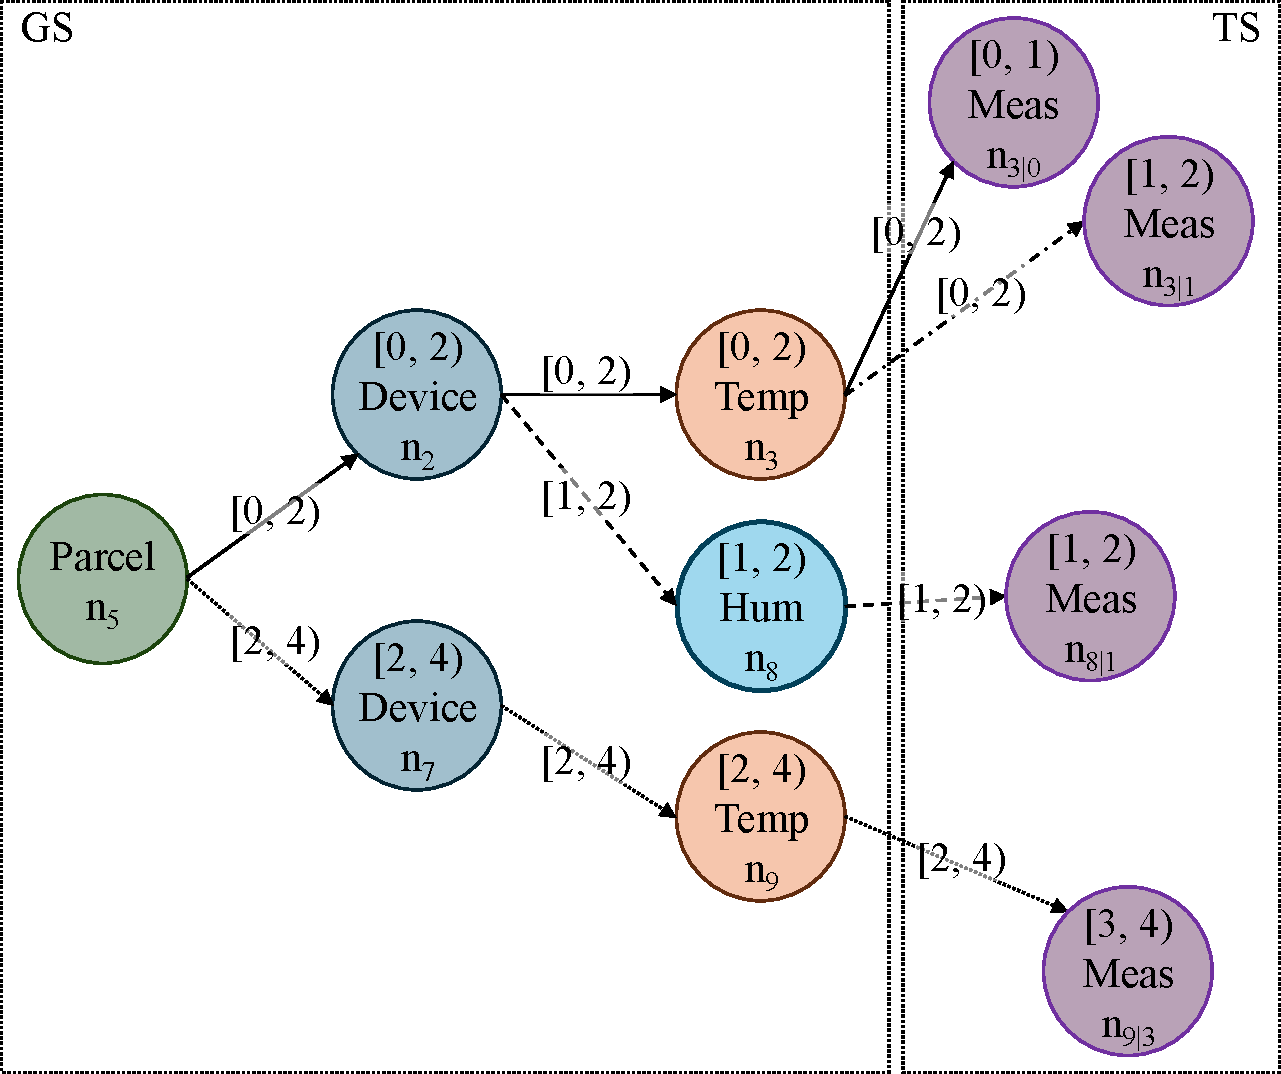
\includegraphics[scale=0.3]{parts/architectures/images/versioning1.pdf}
% \caption{Patterns in the query result with monotonically decreasing temporal validity (from left to right).}\label{fig:versioning1}
% \end{figure}

\begin{example}[Query plan]
In \Cref{fig:example}, $n_2$ was attached to $n_5$ in $[0, 2)$, but then was replaced with $n_7$ in $[2, 4)$.
The Cypher query
\begin{lstlisting}
MATCH (p:Parcel)-[x]->(d:Device)-[y]->(ts)-[z]->(m:Meas)
WHERE p.name = "Parcel 1"
RETURN p, d, ts, m.value
\end{lstlisting}
could have a corresponding query plan $Q$ that is
{\small
\[
\begin{aligned}
R &= \underbrace{\pi_{p,d,ts,m.value}}_{Q[7]}(R_6),&H(R) = (p, d, ts, m.value)\\
R_6 &= \underbrace{\sigma_{m.label = \texttt{Measurement}}}_{Q[6]}(R_5),&H(R_6) = (p, x, d, y, ts, z, m)\\
R_5 &= \underbrace{\varepsilon^{(z,m)}_{ts}}_{Q[5]}(R_4),&H(R_5) = (p, x, d, y, ts, z, m)\\
R_4 &= \underbrace{\varepsilon^{(y,ts)}_d}_{Q[4]}(R_3),&H(R_4) = (p, x, d, y, ts)\\
R_3 &= \underbrace{\sigma_{d.label = \texttt{Device}}}_{Q[3]}(R_2),&H(R_3) = (p, x, d)\\
R_2 &= \underbrace{\varepsilon^{(x,d)}_p}_{Q[2]}(R_1),&H(R_2) = (p, x, d)\\
R_1 &= \underbrace{\sigma_{p.label = \texttt{Parcel}~\land~p.name = ``Parcel~1"}}_{Q[1]}(R_0),&H(R_1) = (p)\\
R_0 &= \underbrace{G^{st}.N}_{Q[0]},&H(R_0) = (p)
\end{aligned}
\]
\noindent where
$R=\begin{array}{|cccc|}
\hline
p & d & ts & m.value \\
\hline
n_5 & n_2 & n_3 & \prop{value}{16} \\
n_5 & n_2 & n_3 & \prop{value}{19} \\
n_5 & n_2 & n_8 & \prop{value}{86} \\
n_5 & n_7 & n_9 & \prop{value}{17} \\
\hline
\end{array}
$, $\ftemporal(t_1)=[0,1), \ftemporal(t_2)=[1,2)$.
}
%\Cref{fig:versioning1} shows the temporal validity (evolving from left to right) of the tuples composing the final relation.
\end{example}

\section{Multistore for graph and time-series}\label{sec:stgraph}

\begin{table}[t]
\centering
\footnotesize
\caption{Data structures of GS and TS. Sizes are in bytes; ``--'' denotes
a variable-size field.}
\label{tbl:structures}
\setlength{\tabcolsep}{4pt}
\begin{tabular}{@{}p{0.23\columnwidth}|
                p{0.23\columnwidth}|
                p{0.23\columnwidth}|
                p{0.23\columnwidth}@{}}
\toprule
\cellcolor{red!20}\textbf{GS Node} &
\cellcolor{blue!20}\textbf{GS Edge} &
\cellcolor{green!20}\textbf{GS Property} &
\cellcolor{orange!20}\textbf{TS Event} \\
\midrule
Id (8)                    & Id (8)                 & Id (8)               & TS id (8) \\
Next property (8)         & Next edge, from (8)    & Next property (8)    & From (8) \\
Next edge (8)             & Next edge, to (8)      & From (8)             & Label (4) \\
From (8)                  & Next property (8)      & To (8)               & Value (8) \\
To (8)                    & From node (8)          & Source id (8)        & Location (--) \\
Label (4)                 & To node (8)            & Source type (1)      & Edges (--) \\
Is TS (1)                 & From (8)               & Type (4)             & Properties (--) \\
                          & To (8)                 & Key (24)             & \\
                          & Label (4)              & Value (8)            & \\
\midrule
\textbf{Total (45)}       &
\textbf{Total (68)}       &
\textbf{Total (77)}       &
\textbf{Total (--)}       \\
\bottomrule
\end{tabular}
\end{table}

\begin{figure}[t]
    \centering
    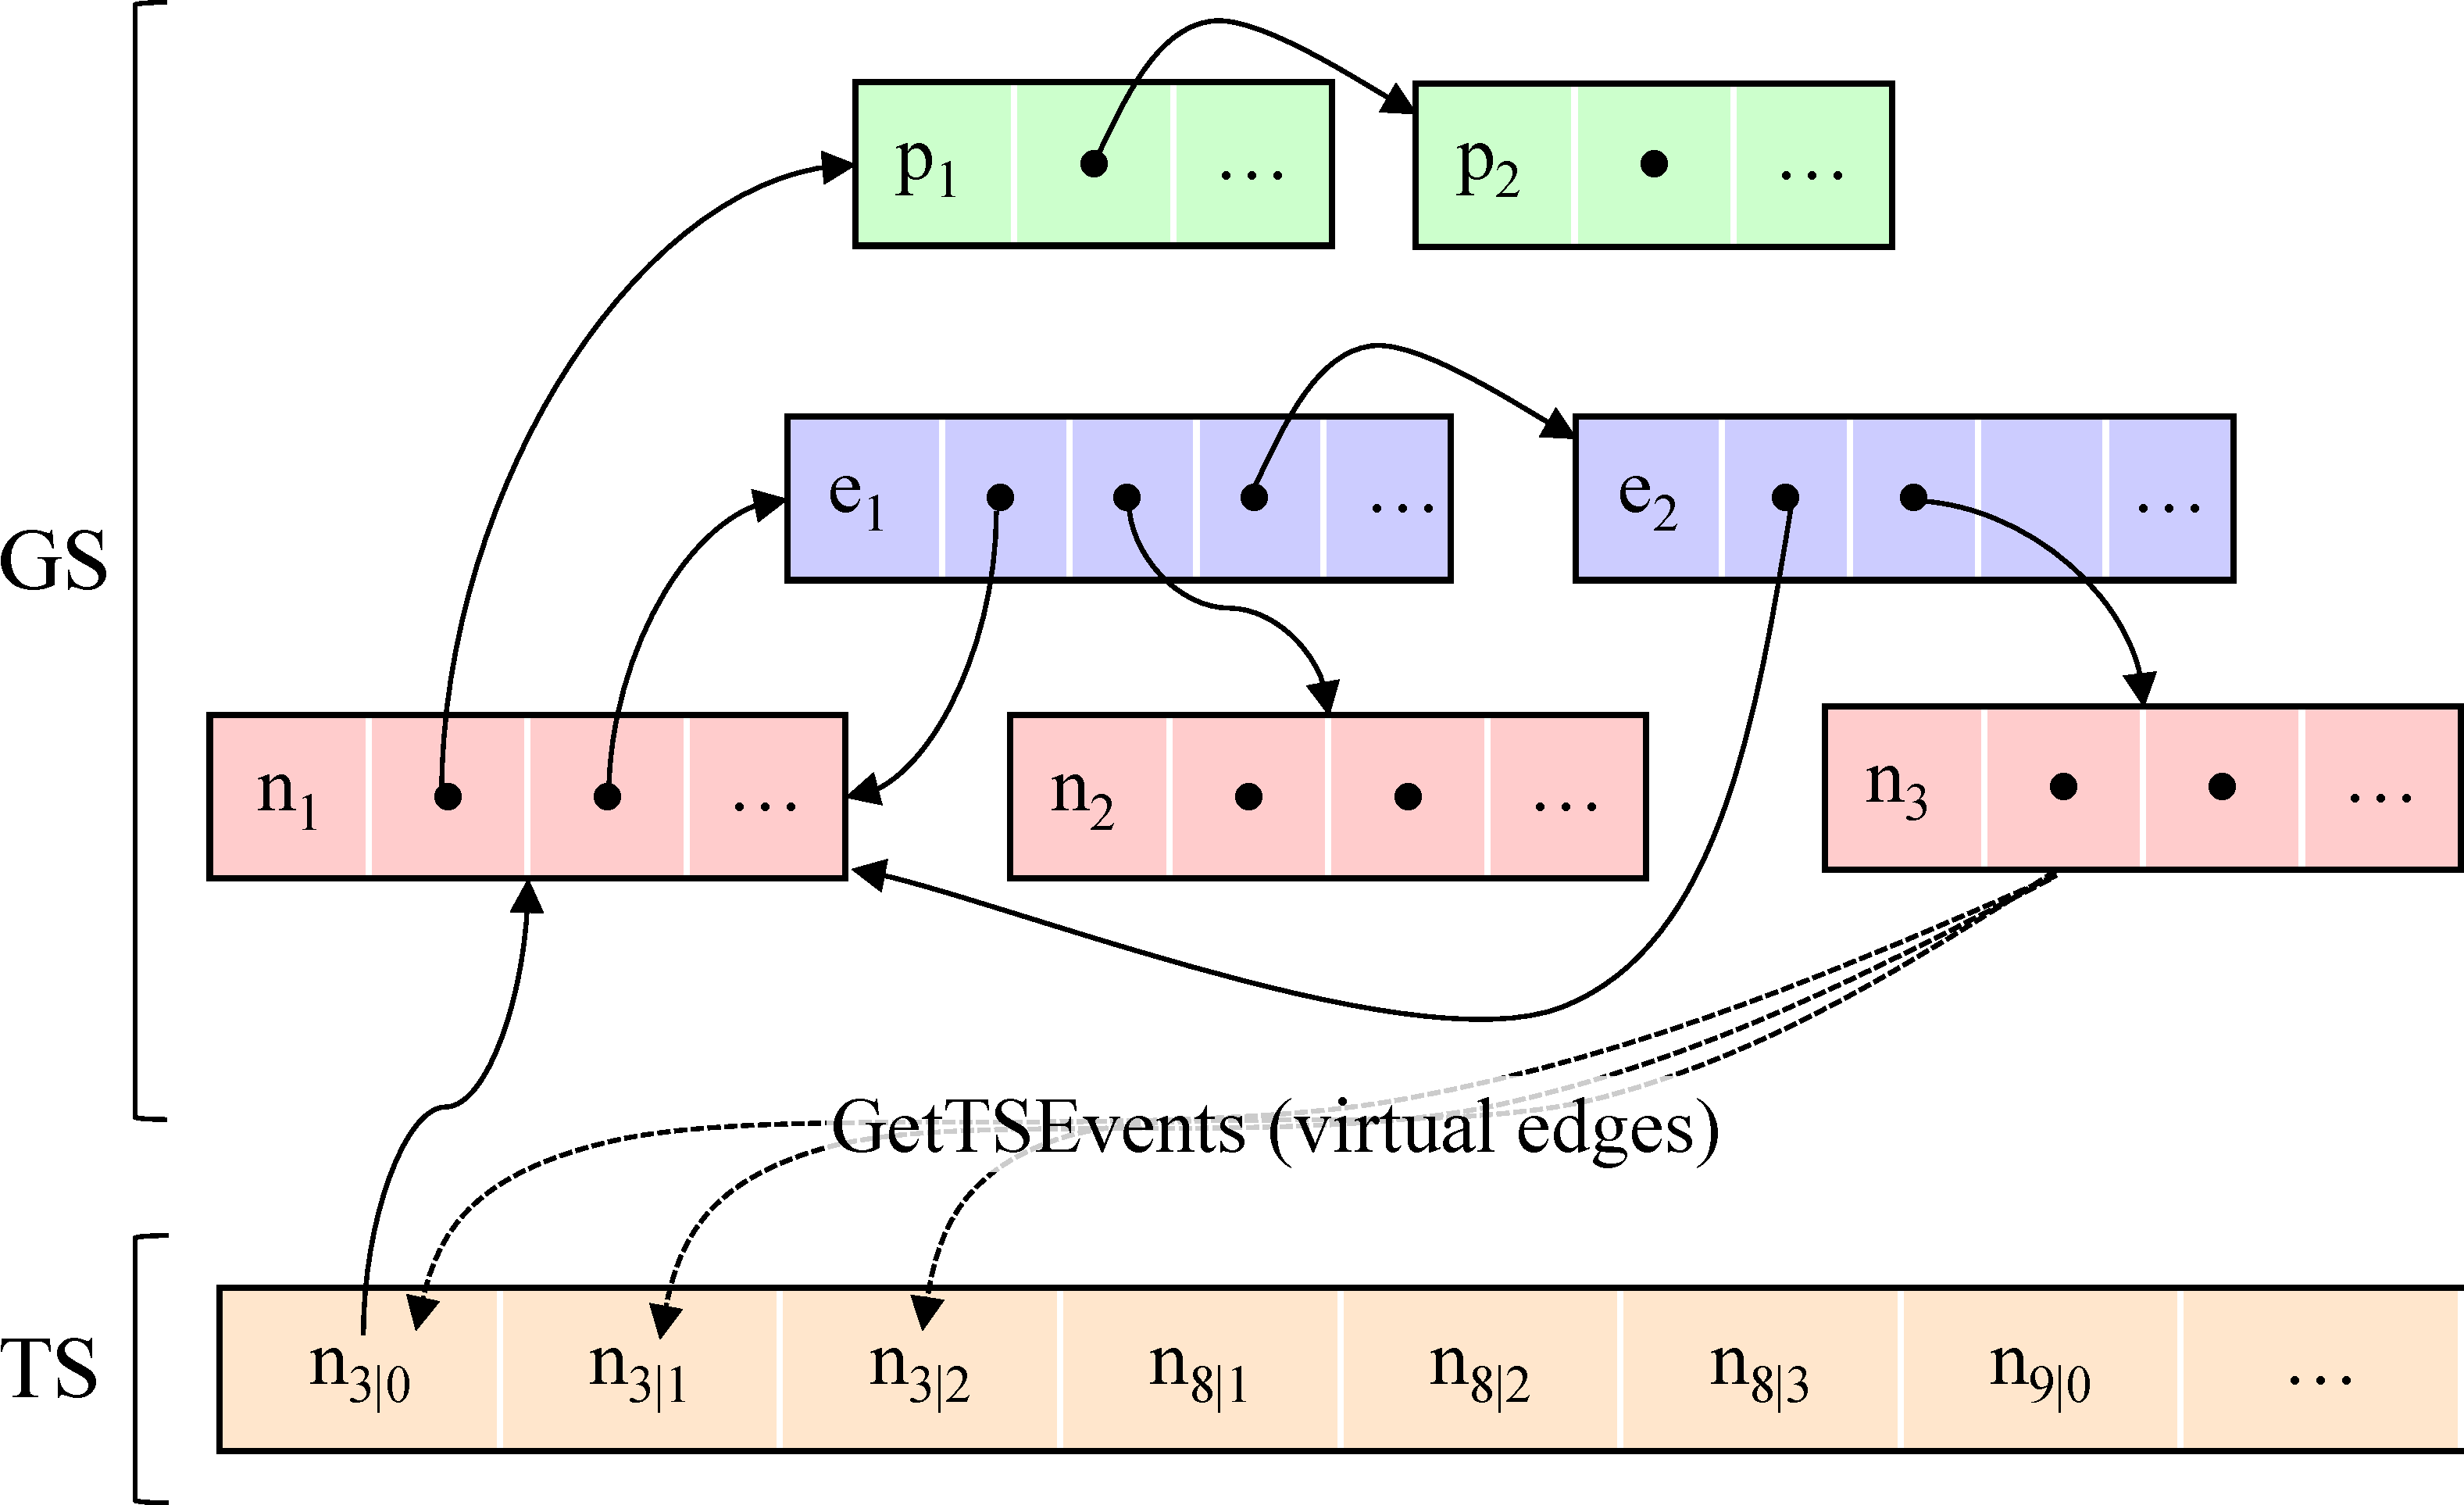
\includegraphics[scale=.145]{parts/architectures/images/overview.pdf}
    \caption{Referring to \Cref{fig:example}, examples of data structures from \Cref{tbl:structures}.
    Events (orange) connected by virtual edges are linked at query time by \textsc{GetTSEvents} in \Cref{alg:search}.}
    \label{fig:structures}
\end{figure}

In \Cref{sec:formal}, we provided \emph{uniform} data and querying abstractions.
From the user's perspective, everything is represented as a spatio-temporal property graph (\Cref{def:stg}).

However, not all graph elements exhibit the same cardinality and access patterns.
Entities such as devices or users are relatively stable and are primarily accessed through graph traversals.
In contrast, temporal events (e.g., measurements) outnumber such entities and are predominantly accessed through temporal filtering, aggregation, and spatial predicates rather than navigation.
Physically storing both using a graph-oriented layout would be suboptimal.%, as graph structures are designed for navigational workloads, whereas event-centric workloads benefit from storage organizations optimized for time-series access.

\subsection{Physical stores}
Following a multistore approach, \ourapproach maps the logical spatio-temporal property graph onto two physical stores.
The Graph Store (GS) persists graph entities and relationships whose primary access pattern is traversal.
The Time-series Store (TS) persists event nodes whose primary access pattern is temporal filtering, aggregation, and spatial lookup.
The two stores are connected through a shared mapping and virtual edges, allowing queries to observe a single spatio-temporal property graph despite the underlying physical separation.
This decoupling allows \ourapproach to inherit the strengths of both physical layouts: it retains structural expressiveness and low-latency graph traversals within GS while ensuring scalable ingestion and querying within TS.
The layouts of the physical stores are summarized in \Cref{tbl:structures} and illustrated in \Cref{fig:structures}.

Referring to \Cref{fig:example}, the logical spatio-temporal property graph includes time-series events as nodes and \lbl{HasEvent} edges. 
% The physical representation (discussed below) preserves this logical abstraction but stores/queries such elements differently.
At query time, time-series events are mapped back to graph nodes, thereby enabling them to hold edges (e.g., $n_{3|0}$ in \Cref{fig:example}) and properties and to serve as traversal points within graph queries.

\subsubsection{Graph Store (GS)}

GS stores nodes, edges, and properties as fixed-size records in independent data structures whose ACID properties are guaranteed through a write-ahead log.
Each GS node stores its temporal validity, a label, a pointer to its first edge, a pointer to its first property, and a flag denoting whether the node owns a time-series in TS (the flag is returned by the function $\fts: N \rightarrow \{true, false\}$).
Each GS edge stores its temporal validity, label, source and destination node identifiers, a pointer to its first property, and next-edge pointers for the adjacency lists of its endpoints.
Each GS property stores its temporal validity, key, value, source identifier, and a next-property pointer.
If the property value fits 8 bytes (e.g., integer, long, or double values or a short UTF-8 String), the value is directly stored in the property.
Otherwise, the value is stored in a key-value Dynamic Store (implemented in RocksDB). % where the key is the ``property id.''

Fixed-size records and pointer chains enable index-free adjacency: traversals follow adjacency lists directly bypassing unrelated records scans or secondary indexes joins.

\subsubsection{Time-series Store (TS)}

%Time-series are long series of events, mostly append-only, and ordered by time.
TS stores all events in a collection distributed on a cluster of machines.
Each event is exposed as a logical graph node, but is physically stored as a variable-size record containing the identifier of its time-series $tsId$, timestamp, label, (nested) properties, (nested) edges, and an optional spatial object.
The primary key of TS collection is $(tsId,timestamp)$, which uniquely identifies an event inside TS.

The collection is indexed by its primary key (and by space through a secondary index) using Log-Structured Merge-tree (LSM-tree) indexes~\cite{DBLP:journals/acta/ONeilCGO96}.
LSM-tree indexes handle highly intensive ingestion workloads efficiently by buffering write operations in memory and periodically flushing them onto disk in batches, making them ideal for continuous ingestion of large volumes of data.

\subsection{Linking and ingesting TS events}
\ourapproach uses a shared mapping to connect GS nodes and TS events.
A GS node or edge identifier $id$ denotes an offset in the corresponding data structure (which stores fixed-size records).
A TS event is addressed by $(tsId,timestamp)$, where $tsId$ identifies the time-series and $timestamp$ identifies the event within that time-series.

Nodes having corresponding time-series in TS are flagged with $\fts(n) = true$ and have a one-to-one mapping with the time-series identifier $tsId$ in TS, i.e., $n.id = tsId$.
This is exploited by the ``Data Collection'' service (\Cref{fig:overview}), enabling each time-series to be continuously ingested independently from GS.
By knowing $tsId$, the decoupled storage allows each event generated by $n$ to be directly appended to the time-series in TS without updating $n$ in GS or materializing a graph edge for each event.
This is how \ourapproach handles high-frequency event streams.
\begin{algorithm}[htp]
\scriptsize
\caption{``Query Service''}
\label{alg:search}
\begin{algorithmic}[1]

\Require Spatio-temporal property graph $G^{st}$, query plan $Q$
\Ensure Relation $R$

\State $R \gets \emptyset$
\label{alg:search:init-result}
\Comment{Result relation}

\State $acc \gets \{(1,(n)) \mid n \in G^{st}.N_{GS}\}$
\label{alg:search:init-acc}
\Comment{Queue accumulator}

\While{$acc$ is not empty}
\label{alg:search:while}
\Comment{Process all pending tuples}

    \State $(i,t) \gets pop(acc)$
    \label{alg:search:pop}

    \item[]
    \Comment{$t$ is the current tuple and $i$ is the index of the operator to be applied to $t$}

    \State $op \gets Q[i]$
    \label{alg:search:get-op}
    \Comment{$op=\varnothing$ if $i \geq |Q|$}

    \Switch{$op$}

        \Case{$\sigma_\theta$}
        \label{alg:search:selection-case}
        \Comment{Selection operator}
            \If{$\sigma_\theta(\{t\}) \ne \varnothing$}
            \label{alg:search:selection-test}
            \Comment{If $t$ satisfies $\theta$}
                \State $acc \gets acc \cup \{(i+1,t)\}$
                \label{alg:search:selection}
            \EndIf
        \EndCase
        
        \Case{$\varepsilon_{a,\theta}^{(x,y)}$}
        \label{alg:search:expand-case}
        \Comment{Expansion operator from node $t[a]$}

            \ForAll{
                $t' \in
                \varepsilon_{a,\theta}^{(x,y)}(\{t\})$
            }
            \label{alg:search:expand-loop}

                \State $acc \gets acc \cup \{(i+1,t')\}$
                \label{alg:search:expand-gs}
                \Comment{Expand edges in GS}

            \EndFor
            \If{$\fts(t[a])$} \Comment{If node $t[a]$ has a corresponding time-series}
                \State $acc \gets acc \cup
                \textsc{QueryTS}(t,a,x,y,i)$
                \label{alg:search:expand-ts}
                \Comment{Expand edges in TS}
            \EndIf

        \EndCase

        \Case{$\pi_A$}
        \label{alg:search:projection-case}
        \Comment{Projection operator}

            \State $acc \gets acc \cup
                \{(i+1,\pi_A(\{t\}))\}$
            \label{alg:search:projection}
            \Comment{Project $t$ and update its schema}

        \EndCase

        \Case{\textbf{default}}
        \label{alg:search:default-case}
        \Comment{No further operator is available}
            \State $R \gets R \cup \{t\}$
            \label{alg:search:result}
            \Comment{Add $t$ to the result relation}
        \EndCase

    \EndSwitch

\EndWhile

\If{$Q[|Q|-1] = \gamma^x_{A,f,a}$}
\label{alg:search:aggregation-test}
\Comment{The last operator is an aggregation}

    \State $R \gets \gamma^x_{A,f,a}(R)$
    \label{alg:search:aggregation}
    \Comment{Group by $A$ and aggregate attribute $a$}

\EndIf

\State \Return $R$
\label{alg:search:return}

\item[]

\Procedure{QueryTS}{$t,a,x,y,i$}
\label{proc:query-push-down}

\Statex \hspace{\algorithmicindent}\textbf{Require:} Tuple $t$, node attr. $a$, edge attr. $x$, event attr. $y$, operator index $i$
\Statex \hspace{\algorithmicindent}\textbf{Ensure:} Tuples extended with virtual edges and time-series events

    \State $n \gets t[a]$
    \label{proc:qpd:get-node}
    \Comment{Retrieve the node bound to attribute $a$}

    \State $acc' \gets \emptyset$
    \label{proc:qpd:init}
    \Comment{Initialize the accumulator}


    \State $\hat{N} \gets \textsc{GetTSEvents}(\{tsId = n.id\}, \varnothing, \varnothing)$
    \label{proc:qpd:query-ts}
    \Comment{Get events from TS}

    \ForAll{$n' \in \hat{N}$}
    \label{proc:qpd:iterate}

        \State $e \gets (n,n')$
        \label{proc:qpd:create-edge}
        \Comment{Construct the virtual edge connecting $n$ and $n'$}

        \State $t' \gets t \cup (e,n')$ \Comment{Extend the tuple, where $H(t')\gets H(t) \cup (x,y)$}
        \label{proc:qpd:extend-tuple}

        \State $acc' \gets acc' \cup \{(i+1,t')\}$
        \label{proc:qpd:add-state}
    \EndFor
    
    \State \Return $acc'$
    \label{proc:qpd:return}

\EndProcedure

\item[]
\Procedure{GetTSEvents}{$\Theta,\Pi,\Gamma$}
\label{proc:query-ts}
\Statex \hspace{\algorithmicindent}\textbf{Require:} Selection predicate $\Theta$, Projection $\Pi$, Aggregation $\Gamma$
\Statex \hspace{\algorithmicindent}\textbf{Ensure:} Events from TS
    \State Implementation of ``Query Rewriter'' (\Cref{fig:overview}), depends on adopted TS engine
\EndProcedure

\end{algorithmic}
\end{algorithm}

\subsection{Querying the spatio-temporal graph}
The seamless querying of GS and TS is carried out by the ``Query Service'' (\Cref{fig:overview} and \Cref{alg:search}).

\Cref{alg:search} describes the execution of a query plan $Q$ over the spatio-temporal property graph $G^{st}$.
The algorithm follows a breadth-first tuple-at-a-time execution based on a queue, denoted by $acc$.
Each element of the queue is a pair $(i,t)$, where $t$ is an intermediate tuple and $i$ identifies the next query operator to be applied to it.
The queue is initialized with one tuple $(n)$ for each node $n \in G^{st}.N_{GS}$\footnote{We start query execution from nodes in GS.}, and each tuple is associated with operator index $1$, since $Q[0]=G^{st}.N_{GS}$ has already produced the initial relation (Line~\ref{alg:search:init-acc}).
Consequently, query evaluation starts independently from every node in the graph.
While the queue is not empty, the algorithm extracts a pair $(i,t)$ (Line~\ref{alg:search:pop}).
It then retrieves the operator $Q[i]$ (Line~\ref{alg:search:get-op}).
If $i \geq |Q|$, no further operator is available and the tuple is considered a final result.
When the current operator is a selection $\sigma_\theta$, the tuple $t$ is evaluated against the predicate $\theta$.
If the predicate is satisfied, the tuple is reinserted into the queue with index $i+1$ (Line~\ref{alg:search:selection}).
Otherwise, the tuple is discarded.
When the current operator is an expansion $\varepsilon_{a,\theta}^{(x,y)}$, the algorithm first evaluates the expansion over GS (each resulting tuple $t'$ is inserted into the queue and associated with the next operator; Line~\ref{alg:search:expand-gs}), then, if the node $t[a]$ has a corresponding time-series, over TS through the $\textsc{QueryTS}$ function; Line~\ref{alg:search:expand-ts}.
The tuples are extended with virtual edges and events are added to the queue.
For a projection operator $\pi_A$, the current tuple is restricted to the attributes in $A$.
The resulting tuple is then associated with index $i+1$ and reinserted into the queue (Line~\ref{alg:search:projection}).
If no operator corresponds to the current index, the tuple has completed the query plan and is inserted into $R$ (Line~\ref{alg:search:result}).
Execution terminates when no additional tuples are in the queue.
Aggregation is handled after all tuples have been collected (Line~\ref{alg:search:aggregation}).
The resulting relation is finally returned (Line~\ref{alg:search:return}).

\paragraph{Traversing time-series nodes}
Since the number of events in TS (e.g., measurements) is significantly higher than the number of nodes in GS (e.g., sensors), physically storing the edges going from GS to TS (\lbl{HasEvent} in \Cref{fig:example}) would require materializing an extremely large number of edges.
%Such a design would not only incur a prohibitive storage overhead but would also negatively impact traversal efficiency.
Instead, we introduce \textit{virtual edges}, i.e. edges that are not physically stored in GS but are generated at query time and returned in the result.

\textsc{QueryTS} (\Cref{alg:search} Line~\ref{proc:query-push-down}) evaluates the expansion towards TS.
%The function receives the current tuple $t$, the id $a$ corresponding to the node from which the expansion starts, the event attribute $y$, and the index $i$ of the current query operator.
First, it retrieves from $t$ the node bound to $a$ (Line~\ref{proc:qpd:get-node}) and initializes an empty set $acc'$ for the tuples produced by the push-down operation (Line~\ref{proc:qpd:init}).
Then, TS is queried using the identifier of $n$ (Line~\ref{proc:qpd:query-ts}).
The query returns a set $\hat{N}$ of events associated with $n$ (i.e., events in TS such that $tsId=n.id$).
For each event $n' \in \hat{N}$, the function constructs a virtual edge $e=(n,n')$ (Line~\ref{proc:qpd:create-edge}) and extends the current tuple $t$ with both the new edge and the event (Line~\ref{proc:qpd:extend-tuple}).
Finally, the function returns all tuples generated through the tuple-store expansion (Line~\ref{proc:qpd:return}).

\paragraph{Traversing events}
Once a TS event is retrieved, it can be traversed by simply filtering its nested edges.

\paragraph{Joining relations}
We do not explicitly incorporate \textsc{Join} into the algorithm since it naturally emerges from the tuple-at-a-time nested-loop evaluation.
In particular, with \Cref{alg:search} we compute the left side of the \textsc{Join}.
For each produced tuple, the same algorithm can then be recursively executed on the right side, using the current tuple as the initial binding.
The tuples returned by the second execution are simply extensions of the original tuple and therefore correspond to the result of a nested-loop join.
Consequently, the \textsc{Join} operator does not require dedicated execution logic and has been omitted from the algorithm for the sake of simplicity.

\section{Query optimization}\label{sec:query}

\begin{figure}[t]
    \centering
    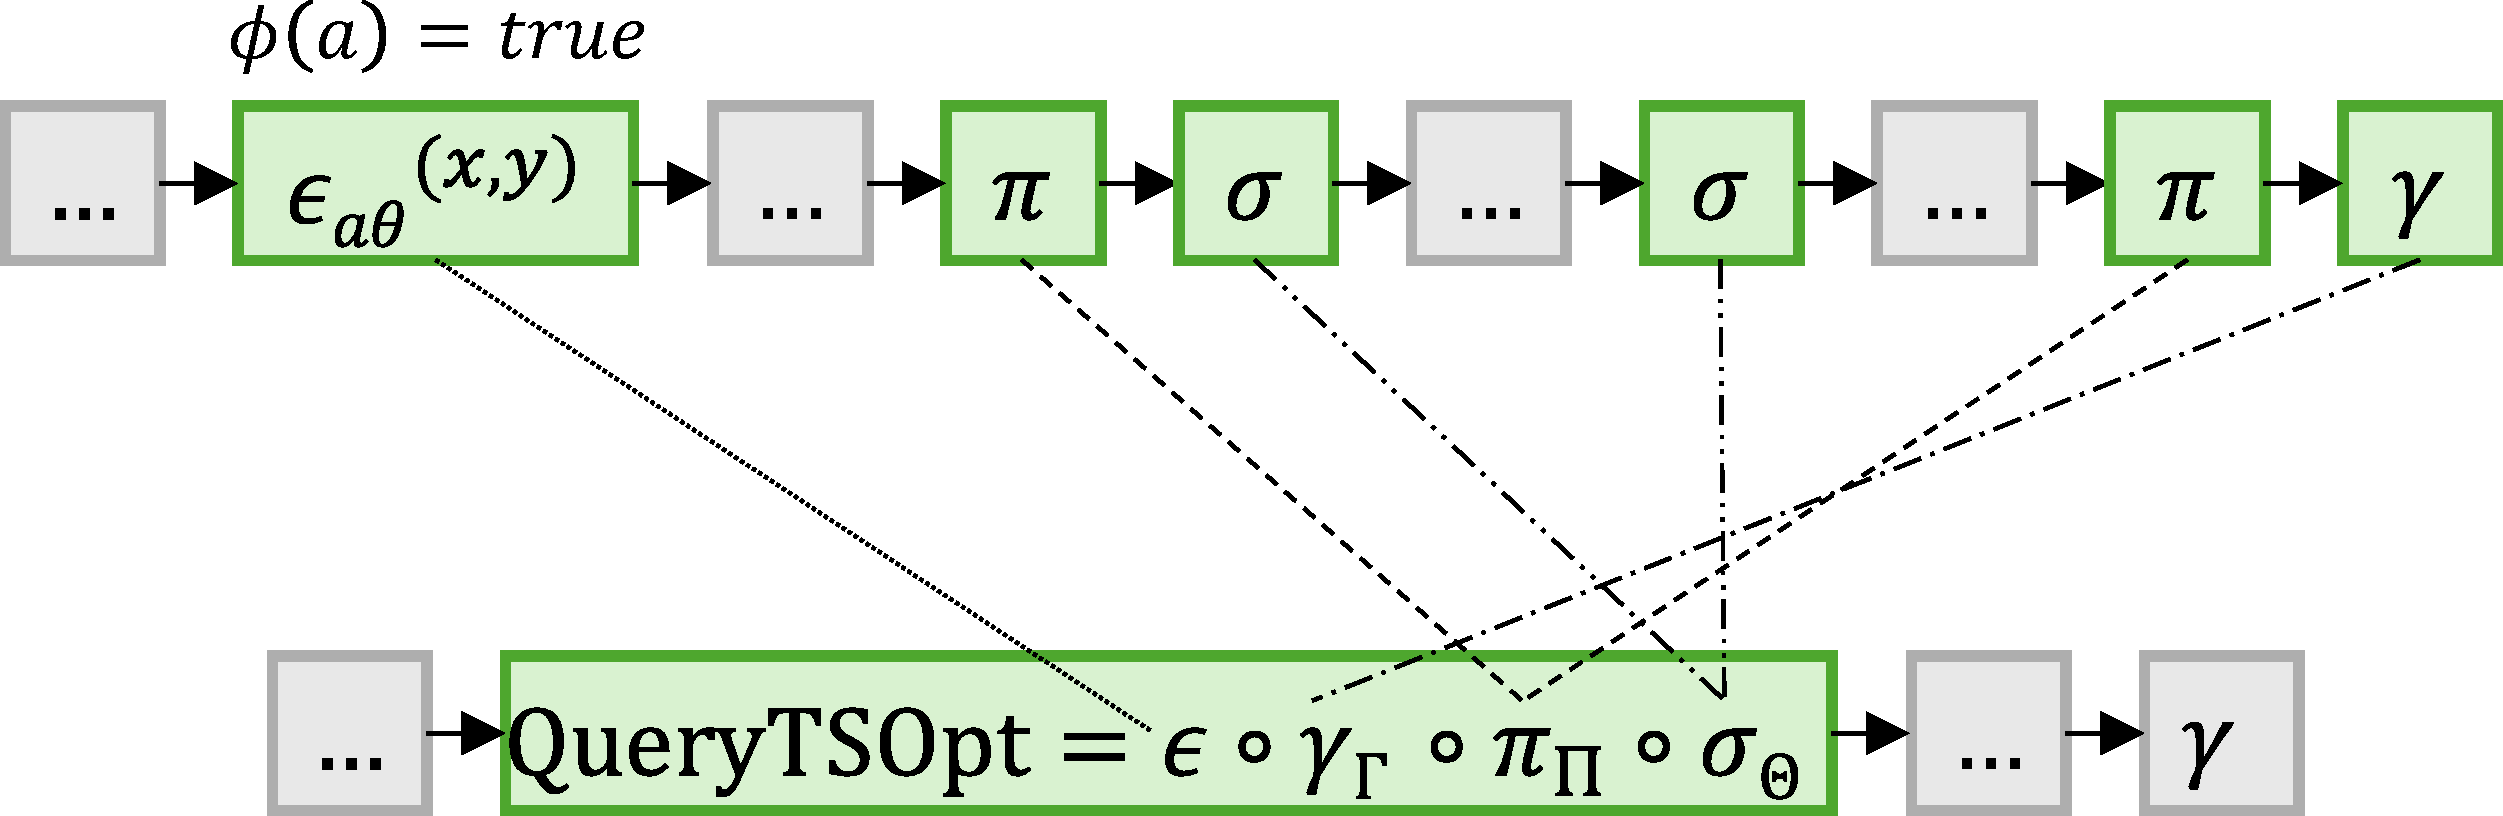
\includegraphics[scale=.18]{parts/architectures/images/opt.pdf}
    \caption{Query optimization to push processing of events down to TS.
    When expanding nodes having corresponding time-series in TS (i.e., $\fts(a)=true$), pushdown is performed by \textsc{QueryTSOpt} (\Cref{alg:query-ts}), which (i) analyzes the query plan to identify predicates, projected properties, and aggregates that depend exclusively on the current time-series variable ($y$), and (ii) fuses and compiles these logical operators into a single physical operator.}
    \label{fig:opt}
\end{figure}

\begin{algorithm}[t]
\footnotesize
\caption{\textsc{QueryTSOpt}}
\label{alg:query-ts}
\begin{algorithmic}[1]

\Require Tuple $t$, node attr. $a$, edge attr. $x$, event attr. $y$, operator idx. $i$, query plan $Q$
\Ensure Tuples extended with virtual edges and time-series events

\Procedure{QueryTSOpt}{$t,a,x,y,i,Q$}
\label{proc:query-ts-opt}

    \State $n \gets t[a]$
    \label{line:qts:get-node}
    \Comment{Retrieve the node bound to $a$}

    \State $acc' \gets \varnothing$
    \label{line:qts:init}
    \Comment{Initialize the result accumulator}

    \State $\Theta \gets \{tsId=n.id\}\cup\textsc{GetPredicates}(t,y,i,Q)$
    \label{line:qts:predicates}
    \Comment{Get the predicates on $y$}

    \State $\Pi \gets \textsc{GetProjectedProperties}(y,i,Q)$
    \label{line:qts:projections}
    \Comment{Get the projections for $y$}

    \State $\Gamma \gets \textsc{GetAggregate}(y,i,Q)$
    \label{line:qts:aggregate}
    \Comment{Get the aggregation by $y$}

    \State $\hat{N} \gets
    \textsc{GetTSEvents}
    \bigl(\Theta,\Pi,\Gamma\bigr)$
    \label{line:qts:query}
    \Comment{Query push down}

    \ForAll{$n' \in \hat{N}$}
    \label{line:qts:iterate}
        \State $e \gets (n,n')$
        \label{line:qts:create-edge}
        \Comment{Construct the virtual edge connecting $n$ and $n'$}
        \State $t' \gets t \cup \{(e,n')\}$
        \label{line:qts:extend}
        \Comment{Extend the tuple, where $H(t')\gets H(t) \cup (x,y)$}
        \State $acc' \gets acc' \cup \{(i+1,t')\}$
        \label{line:qts:accumulate}
    \EndFor
    \State \Return $acc'$
    \label{line:qts:return}
\EndProcedure
\end{algorithmic}
\end{algorithm}

The core contribution of \ourapproach is the transparent cross-store traversal from GS to TS, i.e., the execution boundary where graph traversal expands a node into its associated time-series events.
Consequently, our optimization focuses on this traversal step.
The pushdown towards TS is determined by, and constrained to preserve the semantics of, the portion of the query plan that follows the \textsc{Expand} operator towards time-series events (\Cref{fig:opt}).
Our goal is to find operators in the query plan that can be anticipated and directly computed in TS.
%We optimize the querying of TS when traversing GS nodes.
%As n in \Cref{fig:opt}, our goal is to find operators in the query plan that can be anticipated and directly computed in TS while expanding nodes having a corresponding time-series in TS (i.e., $\fts(a)=true$ in \Cref{fig:opt}).
% When expanding such nodes, 
Pushdown is performed by \textsc{QueryTSOpt} (\Cref{alg:query-ts}) which (i) analyzes the query plan to identify predicates, projected properties, and aggregates that depend on the current time-series variable ($y$), and (ii) fuses and compiles these logical operators into a single physical operator \cite{DBLP:conf/icde/KemperN11,DBLP:conf/cidr/ElgamalLBETRS17} (e.g., logical operators --in green in \Cref{fig:opt}(top)-- are fused into a single physical operator --\Cref{fig:opt}(bottom)).

\textsc{QueryTSOpt} (which replaces \textsc{QueryTS} in \Cref{alg:search}) invokes \textsc{GetPredicates} to construct the set of pushable predicates $\Theta$ (which also includes the predicate $tsId=n.id$; Line~\ref{line:qts:predicates}), \textsc{GetProjectedProperties} (Line~\ref{line:qts:projections}) to determine the set of projected properties $\Pi$, and \textsc{GetAggregate} (Line~\ref{line:qts:aggregate}) to identify an aggregate specification $\Gamma$ that can be delegated to TS.
These operators are compiled together and executed through \textsc{GetTSEvents}.
Consequently, TS returns only the events that satisfy the pushed-down operators.

To simplify the reading of the following algorithms, we will refer to these auxiliary functions.
Given a selection condition $\theta$ (e.g., $\theta = y.val \ge d.thr \land y.ts \ge 10$), $\textsc{Preds}()$ returns the predicates composing the conditions (e.g., $\textsc{Preds}(\theta)=\{y.val \ge d.thr, y.ts \ge 10 \}$) and $\theta$, $\textsc{Operands}()$ returns the single operands (e.g. $\textsc{Operands}(\theta)=\{y.val, d.thr, y.ts\}$ (both excluding constant values).
Given $A \subseteq H(R)$ or a selection condition $\theta$, $\textsc{Attrs}()$ returns the referenced attributes (e.g., $\textsc{Attrs}(\theta)=\{y,d \}$.
Given a single $a \in A$ or operand $p$, $\textsc{Attr}()$ returns the referenced attribute (e.g., $\textsc{Attr}(y.val)=y$).

\subsection{Selection push-down}
\label{subsec:filter-pushdown}

Selection condition can be pushed down to TS to pre-filter events and minimize data shuffling.
A predicate can be pushed to TS only if all of its operands refer to the current time-series (or constants); otherwise, it must be evaluated after the time-series events have been retrieved.
Pushdown is performed by decomposing the selection condition into individual predicates and examining the attributes referenced by each predicate.

\Cref{alg:get-predicates} builds the largest valid predicate $\Theta$ by scanning the suffix of the query plan following $Q[i]$ (Line~\ref{line:gpred:scan}).
Only selection operators are relevant, because they contain predicates that may be evaluated earlier in the plan (Line~\ref{line:gpred:selection}).
A predicate may refer exclusively to $y$ (e.g., $y.ts \ge 10 \land y.ts \le 20$ in green in \Cref{fig:filter-pushdown-example}), or it may also refer to attributes already available in the current tuple (e.g., $y.val \ge d.thr$ in blue in \Cref{fig:filter-pushdown-example}).
The algorithm collects the operands whose attribute is different from $y$ (Line~\ref{line:gpred:external-operands}) since these are external dependencies that prevent the predicate from being directly pushed down.
%The predicate is copied into $pr'$ (Line~\ref{line:gpred:copy}), and each 
Then, each external operand is replaced with its corresponding value from tuple $t$ (Lines~\ref{line:gpred:bind-loop}--\ref{line:gpred:bind}).
For example, given the predicate $y.val \ge d.thr$  and a tuple $t$ such that $t[d].thr = 30$, the binding operation produces $y.val \ge 30$.
The resulting predicate depends only on $y$ and can therefore be pushed down.
%Predicates that already refer only to $y$ have no external operands.
%In that case, the set ($P$) is empty, the binding loop is skipped, and the original predicate is added unchanged to $\Theta$.
%At Line~\ref{line:gpred:add}, each original or bound predicate is inserted into the result set.
Finally, the procedure returns the complete set of pushable predicates at Line~\ref{line:gpred:return}.
A predicate is not pushed down when it does not refer to $y$ or when it refers to another attribute that is not yet present in $H(t)$ (e.g., $y.val \ge z.lim$ in red in \Cref{fig:filter-pushdown-example} since $z$ is introduced by a subsequent expansion and $t[z]$ would be undefined). 

\begin{figure}[t]
\centering
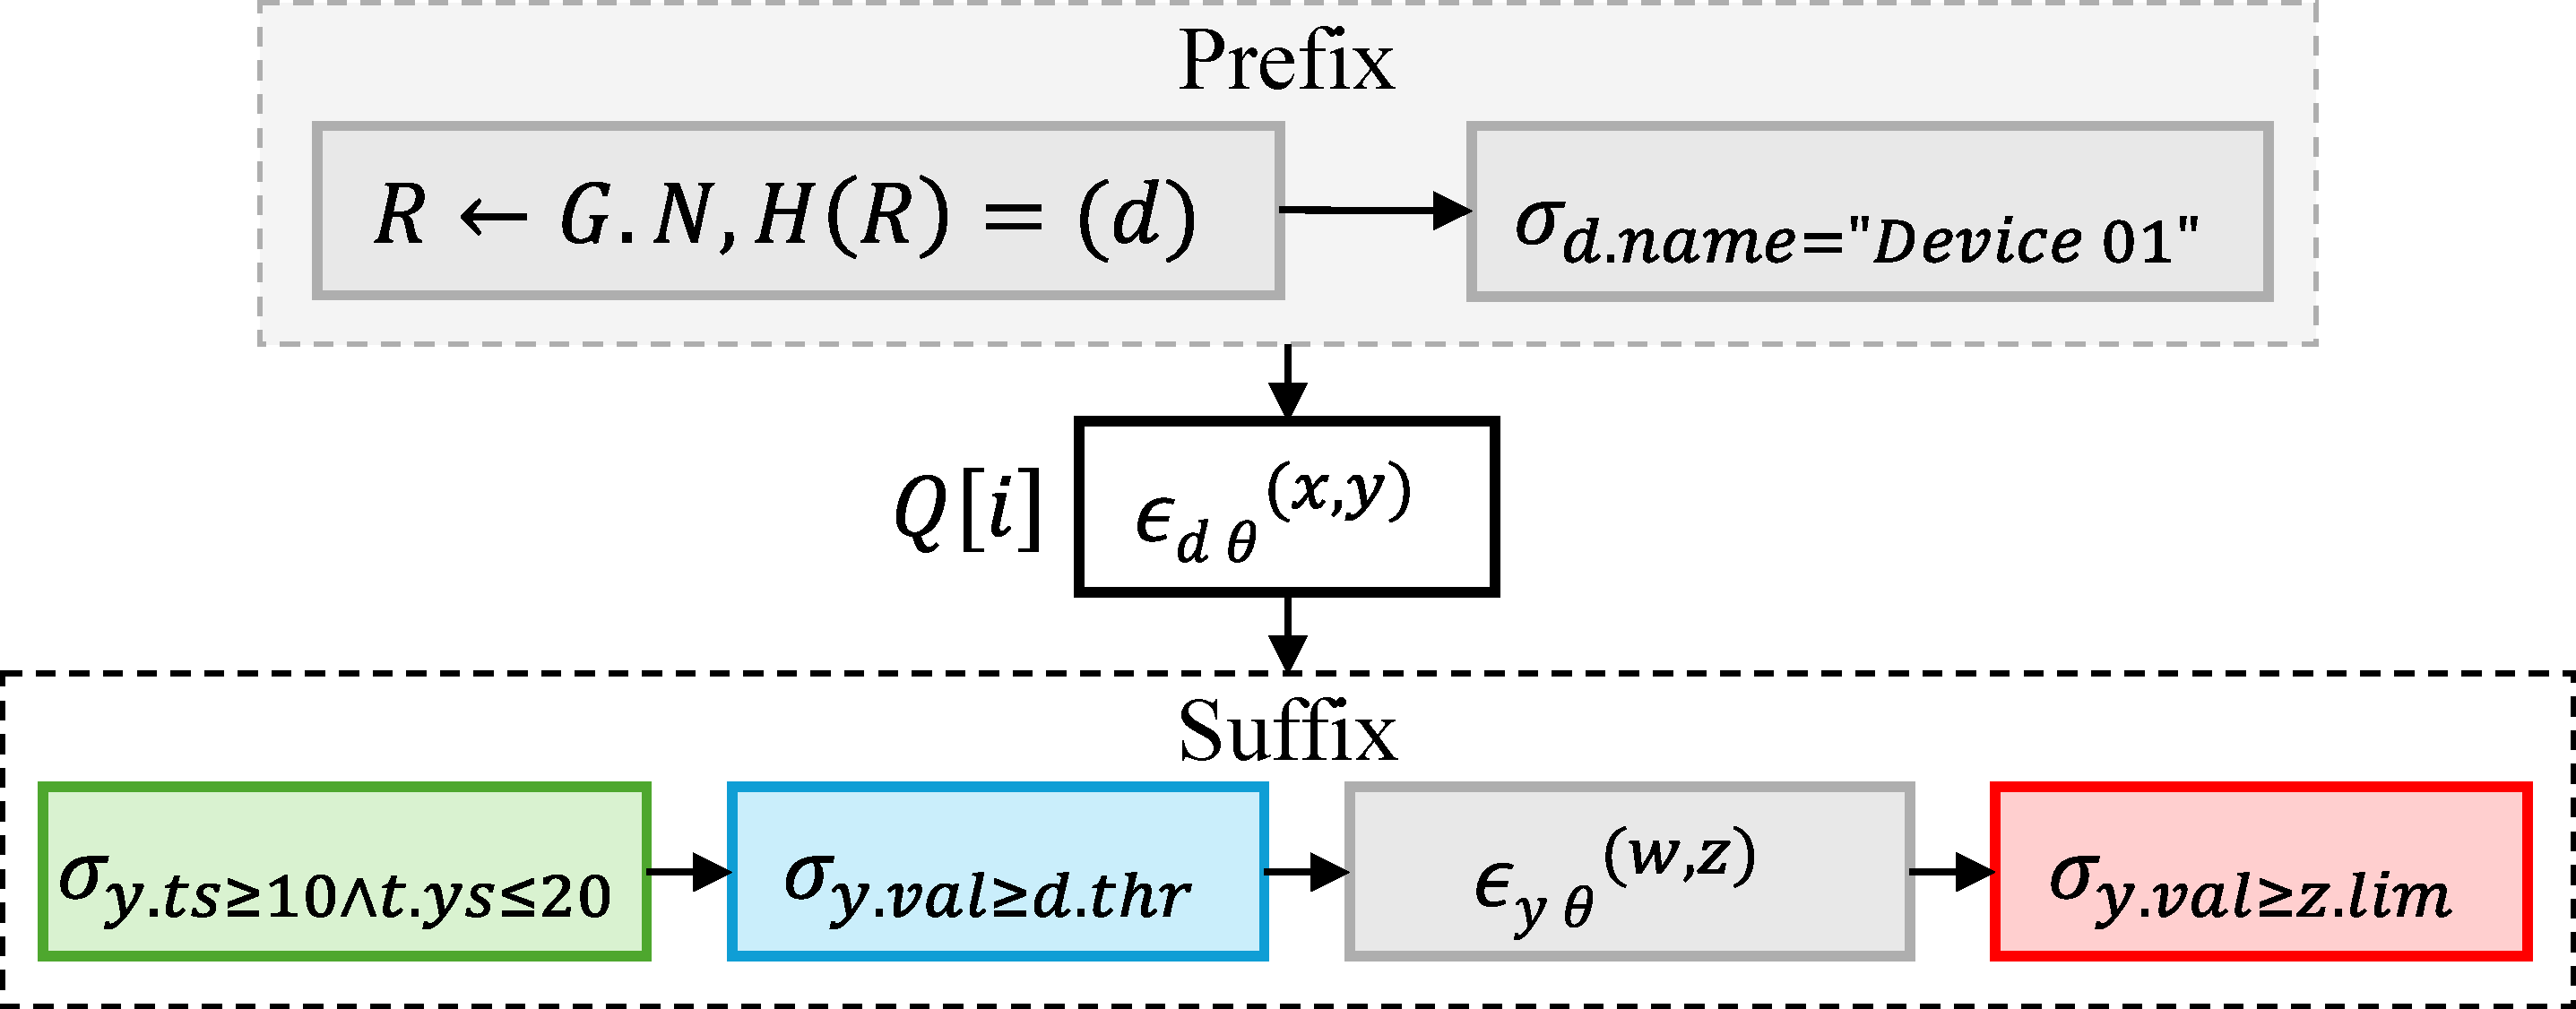
\includegraphics[scale=.165]{parts/architectures/images/filter_pd.pdf}
\caption{
The operator $Q[i]$ expands node $d$ and introduces the edge $x$ and event $y$ attributes.
The predicate $y.ts\ge10\land y.ts\le20$ can be pushed down since it refers only to $y$, while $y.val>d.thr$ can be bound using the value of $d.thr$ since is available when $Q[i]$ is evaluated.
$y.val\ge z.lim$ cannot be pushed down since $z$ is introduced by a subsequent expansion.}
\label{fig:filter-pushdown-example}
\end{figure}

\begin{algorithm}[t]
\scriptsize
\caption{\textsc{GetPredicates}}
\label{alg:get-predicates}
\begin{algorithmic}[1]

\Require Tuple $t$, event attribute $y$, operator index $i$, query plan $Q$
\Ensure Set of predicates $\Theta$

\Procedure{GetPredicates}{$t,y,i,Q$}
    \State $\Theta \gets \varnothing$
    \label{line:gpred:init}
    \Comment{Initialize the set of pushable predicates}

    \For{$op \in Q[i+1:|Q|-1]$}
    \label{line:gpred:scan}
        \Comment{Scan the operators following $Q[i]$}

        \If{$op=\sigma_{\theta}$}
        \label{line:gpred:selection}
            \Comment{Process selection operators only}

            \ForAll{$pr \in \textsc{Preds}(\theta)$}
            \If{$y \in \textsc{Attrs}(pr) \land \bigl(\textsc{Attrs}(pr) \setminus \{y\}\bigr) \subseteq H(t)$}
                \label{line:gpred:predicate-loop}
                \item[]\Comment{Require every attribute other than $y$ to be bound in $t$}
                \State $P \gets
                    \{p \in \textsc{Operands}(pr)
                    \mid \textsc{Attr}(p) \neq y\}$
                \label{line:gpred:external-operands}
                \item[]\Comment{Find operands referring to attributes other than $y$}

                \State $pr' \gets pr$ \Comment{E.g., $pred'\gets y.val \ge d.thr$} 
                \label{line:gpred:copy}

                \ForAll{$p \in P$} 
                \label{line:gpred:bind-loop} \Comment{E.g., $p \gets d.val$}
                    \State $a \gets \textsc{Attr}(p)$ \Comment{E.g., $a\gets d$}
                    \State $k \gets \textsc{Key}(p)$ \Comment{E.g., $k\gets val$}
                    \State $pr' \gets
                        \textsc{Bind}(pr',p,t[a].k)$ {E.g., $pr'\gets y.val \ge 30$}
                    \label{line:gpred:bind}
                    \item[]\Comment{Replace $p$ with its value in the current tuple}
                \EndFor

                \State $\Theta \gets \Theta \cup \{pr'\}$
                \label{line:gpred:add}
                \Comment{Add the predicate}
            \EndIf
            \EndFor
        \EndIf
    \EndFor

    \State \Return $\Theta$
    \label{line:gpred:return}
\EndProcedure

\end{algorithmic}
\end{algorithm}

\subsection{Projection push-down}
\label{subsec:projection-pushdown}

\begin{figure}[t]
    \centering
    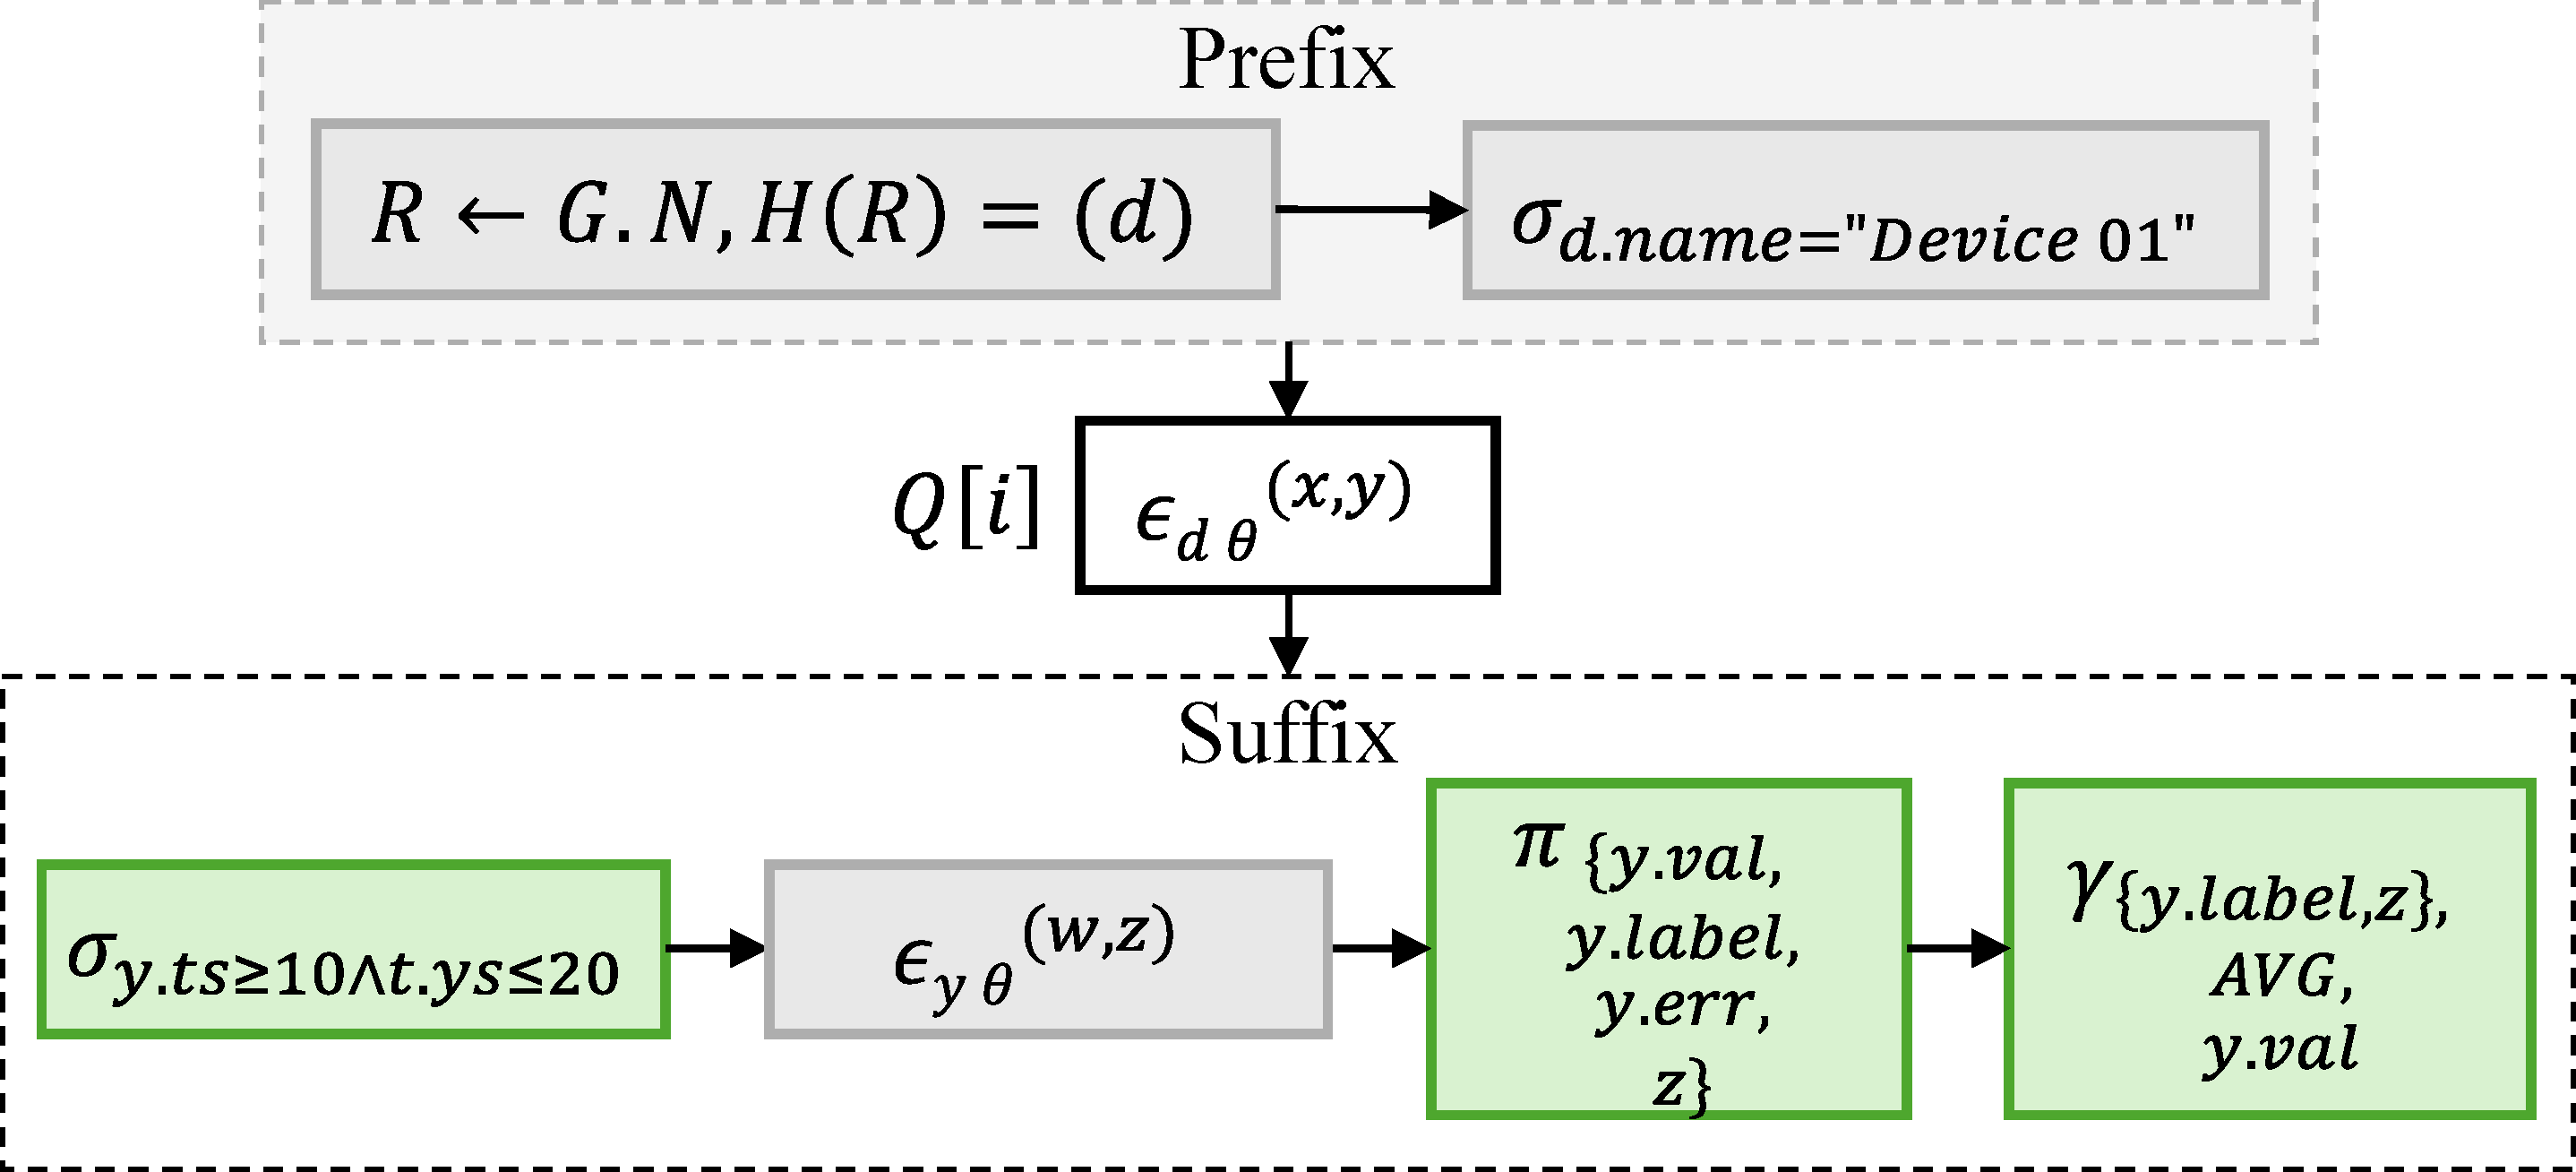
\includegraphics[scale=.165]{parts/architectures/images/projections_pd.pdf}
    \caption{The operator $Q[i]$ expands node $d$ and introduces the edge $x$ and the event $y$ attributes.
    Since the selection, projection, and aggregation requires $y.ts, y.val, y.label, y.err$, only these properties are retrieved for each event in TS.}
    \label{fig:proj-pushdown-example}
\end{figure}

\begin{algorithm}[t]
\scriptsize
\caption{\textsc{GetProjectedProperties}}
\label{alg:get-projections}
\begin{algorithmic}[1]

\Require Event attribute $y$, operator index $i$, query plan $Q$
\Ensure Set of projected properties $\Pi$

\Procedure{GetProjectedProperties}{$y,i,Q$}
\label{proc:get-projections}
    \State $\Pi \gets \emptyset$
    \label{line:gproj:init}
    \Comment{Initialize the set of required properties}
    \ForAll{$op \in Q[i+1:|Q|-1]$}
    \label{line:gproj:scan}
    \Comment{Inspect every operator in the query plan}
        \Switch{$op$}
            \Case{$\pi_A$}
            \label{line:gproj:projection-case}
            \Comment{Process a projection operator}
                \ForAll{$p \in A ~\textbf{s.t.}~ y = \textsc{Attr}(p)$}
                \label{line:gproj:projection-terms}
                \Comment{Properties of $y$}
                    \State $\Pi \gets \Pi \cup \{p\}$
                    \label{line:gproj:add-projection}
                    \Comment{Record the projected property}
                \EndFor
            \EndCase
            \Case{$\sigma_\theta$}
            \label{line:gproj:selection-case}
            \Comment{Process a selection predicate}
                \ForAll{
                    $p \in \textsc{Operands}(\theta)
                    ~\textbf{s.t.}~
                    y = \textsc{Attr}(p)$
                }
                \label{line:gproj:selection-operands}
                \Comment{Operands of $y$}
                    \State $\Pi \gets \Pi \cup \{p\}$
                    \label{line:gproj:add-selection}
                    \Comment{Record the property used by the predicate}
                \EndFor
            \EndCase 
            \Case{$\gamma^x_{A,f,a}$}
            \label{line:gproj:aggregation-case}
            \Comment{Process an aggregation operator}
                \ForAll{$p \in (A \cup \{a\}) ~\textbf{s.t.}~ y = \textsc{Attr}(p)$}
                \label{line:gproj:grouping-terms}
                \Comment{Grouping of $y$}
                    \State $\Pi \gets \Pi \cup \{p\}$
                    \label{line:gproj:add-grouping}
                    \Comment{Record the properties used by aggregation}
                \EndFor
                % \If{$y = \textsc{Attr}(a)$}
                % \label{line:gproj:aggregate-test}
                % \Comment{Check if the aggregation belongs to $y$}
                %     \State $\Pi \gets \Pi \cup \{a\}$
                %     \label{line:gproj:add-aggregate}
                %     \Comment{Record the aggregate argument}
                % \EndIf
            \EndCase
        \EndSwitch
    \EndFor

    \State \Return $\Pi$
    \label{line:gproj:return}
    \Comment{Return all properties of $y$ required to evaluate $Q$}
\EndProcedure

\end{algorithmic}
\end{algorithm}
Projection push-down anticipates the projection to TS to reduce the amount of data transferred across the two stores.
Only the properties required by operators that cannot be pushed down need to be retrieved from TS.
%The set of projected time-series properties is determined by the remaining portion of the query plan: only the properties required by operators that cannot be pushed down need to be retrieved from TS.

\Cref{alg:get-projections} determines which properties must be retrieved by scanning the suffix of the query plan following $Q[i]$ (Line~\ref{line:gproj:scan}).
For a projection operator $\pi_A$, the function examines the projected terms in $A$ (Line~\ref{line:gproj:projection-case}).
Every term $p$ whose attribute refer to $y$ is inserted into $\Pi$ (Line~\ref{line:gproj:add-projection}; e.g., $y.val, y.err, y.label$ in \Cref{fig:proj-pushdown-example}).
% These properties are required because they must be included in the output tuples produced by the projection. 
For a selection operator $\sigma_\theta$, the function examines the operands of $\theta$ (Line~\ref{line:gproj:selection-case}).
An operand is added to $\Pi$ when it references attribute $y$ (Line~\ref{line:gproj:add-selection}).
Such properties must be available to evaluate the corresponding predicates (e.g., $y.ts$ in \Cref{fig:proj-pushdown-example}).
For an aggregation operator $\gamma^x_{A,f,a}$, the function inspects the grouping terms (Line~\ref{line:gproj:aggregation-case}) and those associated with $y$ are added to $\Pi$ (Line~\ref{line:gproj:add-grouping}; e.g., $y.label$ and $y.val$ in \Cref{fig:proj-pushdown-example}).
% The aggregate argument $a$ is then examined separately in Line~\ref{line:gproj:aggregate-test}.
% If it refers to $y$, it is inserted into $\Pi$ in Line~\ref{line:gproj:add-aggregate}, since its value is required to compute the aggregation function $f$ (e.g., $y.val$ in \Cref{fig:proj-pushdown-example}).

\subsection{Aggregate push-down}
\label{subsec:aggregate-pushdown}

\begin{algorithm}[t]
\footnotesize
\caption{\textsc{GetAggregate}}
\label{alg:get-aggregate}
\begin{algorithmic}[1]

\Require Event attribute $y$, operator index $i$, query plan $Q$
\Ensure Aggregate specification $\Gamma$

\Procedure{GetAggregate}{$y,i,Q$}
\label{proc:get-aggregate}
    \State $\Gamma \gets \varnothing$
    \If{$\not\exists op \in Q[i+1:|Q|-1]~\textbf{s.t.}~op=\varepsilon^{w,z}_{a,\theta} \land a = y$}\label{line:ga:expand-check}
        \item[]\Comment{No further expand on $y$} 

        \For{$op \in Q[i+1: |Q| - 1]$}

        \If{$op=\gamma_{A,f,a}^w \land f\textup{ is not holistic } \land y = \textsc{Attr}(a)$}\label{line:ga:aggregate-check}\Comment{Aggregate $y$} 
            \State $\Gamma \gets
            \left(
                \{p \in A \mid y = \textsc{Attr}(p)\},
                f,
                a
            \right)$
            \label{line:ga:construct}
            \Comment{Aggregate specification}
        \EndIf
        \EndFor
    \EndIf
    \State \Return $\Gamma$
    \label{line:ga:return-empty}
\EndProcedure
\end{algorithmic}
\end{algorithm}
If possible, aggregation push-down anticipates the execution of aggregation operators in TS, thereby reducing the amount of data transferred and exploiting the superior efficiency of TS for aggregating large collections of events.
An aggregation can be delegated when its aggregate argument depends on the current time-series.
As a result, TS returns aggregated values instead of raw events, substantially reducing both data transfer and processing by the query engine.
For distributive aggregation functions (e.g., $\{\mathrm{COUNT}, \mathrm{SUM}, \mathrm{MIN}, \mathrm{MAX}\}$), \textsc{GetTSEvents} computes partial aggregates over TS and \Cref{alg:search} later combines these partial results to obtain the final global aggregate.
Since distributive functions are associative and composable, this optimization preserves the exact query semantics while significantly reducing the amount of data transferred between the two stores.
Algebraic aggregation functions, such as $\mathrm{AVG}$, are handled by computing the corresponding partial aggregates in TS (e.g.,  $\{\mathrm{COUNT}, \mathrm{SUM}\}$) and eventually combining them to derive the final result.
Holistic aggregation functions (e.g., $\mathrm{MEDIAN}$) cannot be decomposed into independent partial aggregates.

\Cref{alg:get-aggregate} identifies whether an aggregation involving the event attribute $y$ can be pushed down.
% The function \textsc{GetAggregate}, identified by \Cref{proc:get-aggregate}, receives the event attribute $y$, the index $i$ of the current operator, and the query plan $Q$.
The function verifies that the portion of the query plan following position $i$ does not contain an expansion operator whose source attribute is $y$ (Line~\ref{line:ga:expand-check}).
A subsequent expansion from $y$ requires the original event instances to remain available; therefore, aggregating them in advance could discard information required by the expansion.
If no such expansion exists, the function scans the operators occurring after position $i$.
For each operator, it checks whether the operator is a not-holistic aggregation $\gamma^w_{A,f,a}$ where $a$ belongs to event attribute $y$ (Line~\ref{line:ga:aggregate-check}; e.g., $\gamma_{\{y.label,z\},\mathrm{AVG},y.val}$ in \Cref{fig:proj-pushdown-example}).
If so, the function constructs the aggregate specification $\Gamma$ (Line~\ref{line:ga:construct}), where the first component contains the grouping properties in $A$ associated with $y$ (e.g., $\{y.label\}$), $f$ is the aggregation function, and $a$ is the property over which the aggregation is evaluated (e.g., $y.val$).
Grouping attributes not associated with $y$ (e.g., $z$) are eventually considered when combining the partial aggregates.

\subsection{Multi-threaded query execution}
\label{subsec:query-parallel-execution}

For both \textsc{QueryTS} and \textsc{QueryTSOpt}, the invocation of \textsc{GetTSEvents} can be executed concurrently since the TS requests are independent for each tuple.
% For instance, in \textsc{QueryTSOpt} (\Cref{alg:query-ts}), each invocation retrieves the node bound in its own tuple at Line~\ref{line:qts:get-node} and independently constructs its filter, projection, and aggregate specifications at Lines~\ref{line:qts:predicates}--\ref{line:qts:aggregate}.
% Once these parameters have been derived, the request issued at Line~\ref{line:qts:query} depends only on the bindings contained in the corresponding tuple and does not depend on the results of requests generated for other tuples.
Given an input relation
$
    R=\{t_i,\ldots\},
$
the ``Query Service'' can generate one request 
$
    \textsc{GetTSEvents}
    \bigl(
        \Theta_i,
        \Pi_i,
        \Gamma_i
    \bigr)$
for each tuple $t_i$
.
This independence enables a multi-threaded execution in which the requests are submitted to a pool of worker threads.
Each worker sends one request to TS and processes the returned events by performing the tuple-extension operations.

Parallel execution is effective when time-series retrieval is I/O-bound or when TS supports concurrent requests, since latency is determined by the slowest batch rather than by the sum of all requests.
The degree of parallelism must be bounded to avoid overloading TS or exhausting network connections.
Our implementation uses a fixed-size thread pool, sized according to the resources of the ``Query Service'' and the concurrency supported by TS, whose workers update a thread-safe shared accumulator.

\section{Experimental evaluation}\label{sec:exp}

\begin{table}[t]
\centering
\footnotesize
\caption{Dataset statistics.}
\label{tab:datasets}
\begin{tabular}{lcccc}
\toprule
Dataset       & Size & Nodes & Edges & Avg.
TS events\\
\midrule
\multirow{3}{*}{\textsf{MIV}} & S    & $1.7 \cdot 10^6$   & $1.7 \cdot 10^6$ & $2.5 \cdot 10^3$ \\
              & M    & $1.7 \cdot 10^7$   & $1.7 \cdot 10^7$ & $2.5 \cdot 10^3$ \\
              & L    & $1.7 \cdot 10^8$   & $1.7 \cdot 10^8$ & $2.6\cdot10^3$ \\\midrule
\multirow{3}{*}{\textsf{SB}}  
              & S    & $2.5\cdot10^{6}$   & $2.5\cdot10^{6}$ & $2.5\cdot10^{4}$ \\
              & M    & $1.0\cdot10^{7}$   & $1.0\cdot10^{7}$ & $5.1\cdot10^{4}$ \\
              & L    & $2.6\cdot10^{8}$   & $2.6\cdot10^{8}$ & $2.5\cdot10^{5}$ \\
              & XL   & $3.0\cdot10^{8}$   & $3.0\cdot10^{8}$ & $1.5\cdot10^{6}$ \\
\bottomrule
\end{tabular}

%\begin{table}[t]
%\centering
%\footnotesize
\caption{Characteristics of query workload.}
\label{tab:queries}
\begin{tabular}{lcccccccc}
\toprule
           &    & \multicolumn{2}{c}{Store} & \multicolumn{5}{c}{Operators}\\
           \cmidrule(lr){3-4}\cmidrule(lr){5-9}
Dataset  & ID & GS        & TS          & Join                & Aggregate     & Select    & Expand        & Project   \\\midrule
\multirow{3}{*}{\textsf{SB}}& Q1 & \ding{51} &             &                     &               & \ding{51} & \ding{51}     & \ding{51} \\
           & Q2 & \ding{51} & \ding{51}   & \ding{51}           & \ding{51}     & \ding{51} & \ding{51}     & \ding{51} \\
           & Q3 & \ding{51} & \ding{51}   & \ding{51}           &               & \ding{51} & \ding{51}     & \ding{51} \\
           & Q4 & \ding{51} & \ding{51}   & (spatial)           & \ding{51}     & \ding{51} & \ding{51}     & \ding{51} \\
           & Q5 & \ding{51} & \ding{51}   &                     & \ding{51}     & \ding{51} & \ding{51}     & \ding{51} \\
           & Q6 & \ding{51} &             &                     & \ding{51}     & \ding{51} & \ding{51}     & \ding{51} \\\midrule
\multirow{3}{*}{\textsf{MIV}}  & Q1 & \ding{51} &             &                     &               & \ding{51} & \ding{51}     & \ding{51} \\
           & Q2 & \ding{51} & \ding{51}   &                     & \ding{51}     &           & \ding{51}     & \ding{51} \\
           & Q3 & \ding{51} & \ding{51}   &                     & \ding{51}     & \ding{51} & \ding{51}     & \ding{51} \\
\bottomrule
\end{tabular}
\end{table}

The implementation and evaluation of \ourapproach is available at \url{https://github.com/big-unibo/stgraph}.
GS is centralized and runs on a single machine, while TS is distributed across multiple machines in a cluster.
GS has been developed in Kotlin and TS has been implemented in AsterixDB~\cite{DBLP:journals/pvldb/AlsubaieeAABBBCCCFGGHKLLOOPTVWW14}.
Time-series are stored as an AsterixDB dataset of records partitioned across nodes in a cluster and indexed through LSM-tree indexes~\cite{DBLP:journals/pvldb/AlsubaieeBBHKCDL14}.
AsterixDB also supports secondary indexes, including a spatial LSM R-tree~\cite{DBLP:journals/pvldb/AlsubaieeBBHKCDL14} used to index the \texttt{location} property and Data Feeds~\cite{DBLP:conf/edbt/GroverC15} to implement high-throughput ingestion adapters for time-series data.
%
% A Data Feed allows the definition of an ingestion pipeline that maps incoming data from an external source (operating in either push or pull mode) directly into existing datasets.
%
% \ourapproach assigns a dedicated data feed to each time-series node, enabling parallel streaming ingestion across multiple data sources.
%
The storage replication factor in AsterixDB was fixed to 1 to take into account raw storage costs only.

Experiments were conducted on a cluster of machines equipped with an Intel Xeon W5-2445 processor (20 cores, 4.6 GHz) and 256 GB of DDR5 RAM.
%In the following, we first describe the datasets and queries used for testing, and then we present the results of the evaluation.

\subsection{Datasets}

For the testing datasets, \Cref{tab:datasets} summarizes the number of nodes and edges and the average time-series length. 
Overall, (1) \textsf{MIV} contains thousands of shorter time-series (up to $2.6 \cdot 10^3$ events on average), while \textsf{SB} contains fewer but longer time-series (up to $1.5\cdot10^6$ events on average), and (2) the number of time-series events is orders of magnitude higher than the volume of master data, which motivates the need for a hybrid data structure and optimized query execution.

\subsubsection{Medical Information Mart for Intensive Care IV (\textsf{MIV})}

\textsf{MIV} \cite{johnson2020mimic} is a large deidentified dataset of patients admitted to the emergency department or an intensive care unit.
It contains data for patients admitted to an ICU and incorporates health-care time-series data.
Large is the full version of the dataset, while Small ($\times\frac{1}{100}$) and Medium ($\times\frac{1}{10}$) are downscaled versions.
Mimic queries range over the whole graph.
Q1 filters on healthcare events.
Q2 computes the average values of all time-series.
Q3 combines Q1 and Q2 by averaging values of filtered time-series. 

\subsubsection{SmartBench (\textsf{SB})}
\textsf{SB}~\cite{DBLP:journals/pvldb/GuptaCMY20} is a benchmark derived from a real-world smart building monitoring system.
It models devices composed of sensors performing high-frequency measurements and the spatial structure of the monitored environment.
\textsf{SB} provides a tool to generate datasets of increasing scaling factors: Small ($\times1$), Medium ($\times4$), and Large ($\times100$); XL is a variation of M with artificially-extended time-series.

\textsf{SB} also defines queries that differ in terms of filtering conditions, aggregation functions, and selection criteria.
The characteristics of the queries selected for evaluation are detailed in \Cref{tab:queries} (the complete specification of the queries can be found in \cite{DBLP:journals/pvldb/GuptaCMY20}).
Q1 is a graph traversal query that does not require access to TS.
Q2 and Q5 are analytical queries; Q2 has a high-selectivity filter (it includes $\approx12\%$ events), while Q5 has a low-selectivity filter (it includes $\approx37\%$ of events).
Q3 and Q4 join graph nodes and time-series events based on existence conditions on specific events.
Q4 involves a spatial join operation, since a device may produce data within an environment without being explicitly connected to it through a graph edge. 
Finally, Q6 gets all the historical relationships of a sensor, including all past measurements.

\subsection{Pushdown: \textsc{QueryTS} vs \textsc{QueryTSOpt}}

\Cref{fig:opt_vs_naive} and \Cref{tbl:opt_vs_naive} compare the performance of \textsc{QueryTS} and \textsc{QueryTSOpt} (see \Cref{sec:query}); intuitively, \textsc{QueryTS} collects all data before processing it, while \textsc{QueryTSOpt} pushes event processing down to TS.
GS and TS run on the same machine and use 1 thread.

\textsc{QueryTSOpt} consistently outperforms \textsc{QueryTS}.
For the \textsf{MIV} dataset, execution times are reduced by approximately one order of magnitude, while on the more demanding \textsf{SB} workload the gains are even larger, reaching or exceeding two orders of magnitude for the most time-series-intensive queries (Q1 in \textsf{SB} is not affected by the optimization since it only involves operations on GS). 
Moreover, \textsc{QueryTS} does not complete within practical limits (marked as \oot) for several query-dataset combinations.
The benefits of \textsc{QueryTSOpt} become more pronounced as time-series length and data scan increase (e.g., less selective predicates or group by on the whole time-series), confirming the effectiveness of the proposed optimizations.
This is particularly evident in \textsf{SB} Q3 that must verify whether each time-series satisfies a given condition (e.g., contains at least one measurement above a threshold).
While \textsc{QueryTS} shuffles all data back to GS, \textsc{QueryTSOpt} directly checks the time-series in TS and only returns the relevant information, resulting in speedups of orders of magnitude.

\begin{figure}[t]
    \centering
    \begin{subfigure}[t]{\columnwidth}
        \centering
        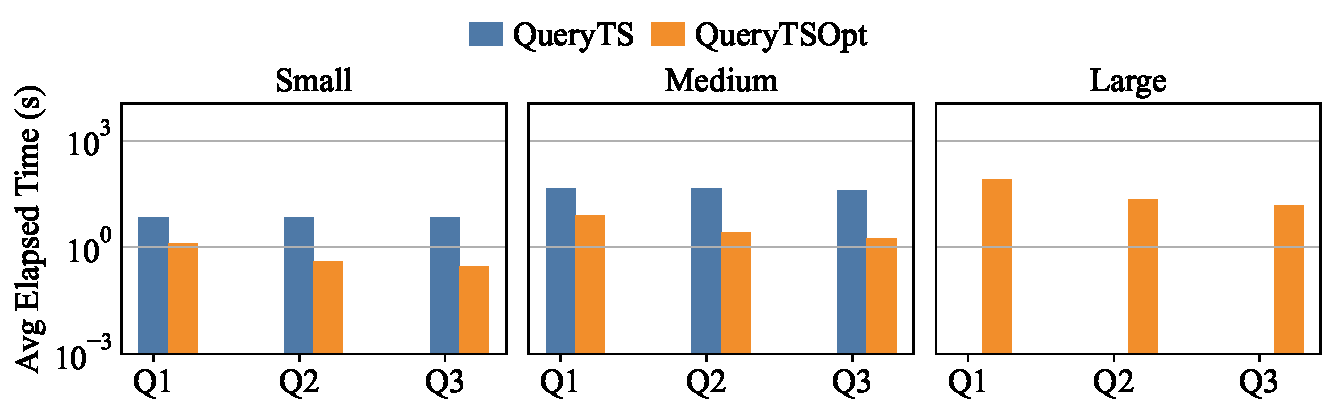
\includegraphics[scale=.6]{parts/architectures/images/query_opt_mimic.pdf}
        \caption{\textsf{MIV}}
    \end{subfigure}
    \begin{subfigure}[t]{\columnwidth}
        \centering
        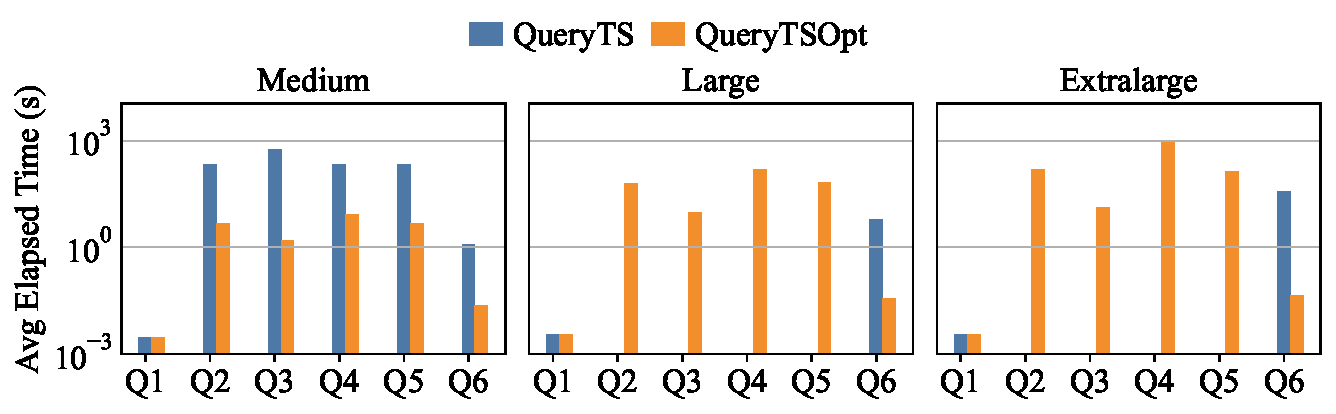
\includegraphics[scale=.6]{parts/architectures/images/query_opt_smartbench.pdf}
        \caption{\textsf{SB}}
    \end{subfigure}
    \caption{\textsc{QueryTS} vs \textsc{QueryTSOpt}.
For both \textsf{SB} and \textsf{MIV}, \textsc{QueryTS} fails to compute for queries accessing too much data.
For the sake of space, \textsf{SB}-Small has been omitted.
}
\label{fig:opt_vs_naive}
\end{figure}

\begin{table}[t]
\centering\footnotesize
\caption{\textsc{QueryTS} vs \textsc{QueryTSOpt}.}
\label{tbl:opt_vs_naive}
\setlength{\tabcolsep}{2.5pt}
\renewcommand{\arraystretch}{0.9}
\resizebox{\columnwidth}{!}{%
\begin{tabular}{lcccccccc}
\toprule
 &  & & Q1 & Q2 & Q3 & Q4 & Q5 & Q6 \\
Dataset & Size & Mode &  &  &  &  &  &  \\
\midrule
\multirow[*]{5}{*}{\textsf{MIV}} & \multirow[*]{2}{*}{S} & \textsc{QueryTS} & $6.8 \cdot 10^{0}$ & $7.1 \cdot 10^{0}$ & $7.2 \cdot 10^{0}$ & -- & -- & -- \\
 &  & \textsc{QueryTSOpt} & $1.3 \cdot 10^{0}$ & $4.0 \cdot 10^{-1}$ & $3.0 \cdot 10^{-1}$ & -- & -- & -- \\
\cline{2-9}
 & \multirow[*]{2}{*}{M} & \textsc{QueryTS} & $4.7 \cdot 10^{1}$ & $4.6 \cdot 10^{1}$ & $3.9 \cdot 10^{1}$ & -- & -- & -- \\
 &  & \textsc{QueryTSOpt} & $7.9 \cdot 10^{0}$ & $2.6 \cdot 10^{0}$ & $1.8 \cdot 10^{0}$ & -- & -- & -- \\
\cline{2-9} & \multirow[*]{2}{*}{L} & \textsc{QueryTS} & \oot & \oot & \oot & -- & -- & -- \\
 &  & \textsc{QueryTSOpt} & $7.9 \cdot 10^{1}$ & $2.2 \cdot 10^{1}$ & $1.5 \cdot 10^{1}$ & -- & -- & -- \\
\midrule
\multirow[*]{8}{*}{\textsf{SB}}  & \multirow[*]{2}{*}{S} & \textsc{QueryTS} & $1.5 \cdot 10^{-3}$ & $5.7 \cdot 10^{1}$ & $1.0 \cdot 10^{2}$ & $6.2 \cdot 10^{1}$ & $5.2 \cdot 10^{1}$ & $6.3 \cdot 10^{-1}$ \\
 &  & \textsc{QueryTSOpt} & $1.5 \cdot 10^{-3}$ & $2.0 \cdot 10^{0}$ & $8.0 \cdot 10^{-1}$ & $2.9 \cdot 10^{0}$ & $1.8 \cdot 10^{0}$ & $1.3 \cdot 10^{-2}$ \\
\cline{2-9}
 & \multirow[*]{2}{*}{M} & \textsc{QueryTS} & $3.0 \cdot 10^{-3}$ & $2.2 \cdot 10^{2}$ & $5.9 \cdot 10^{2}$ & $2.2 \cdot 10^{2}$ & $2.1 \cdot 10^{2}$ & $1.2 \cdot 10^{0}$ \\
 &  & \textsc{QueryTSOpt} & $3.0 \cdot 10^{-3}$ & $4.7 \cdot 10^{0}$ & $1.5 \cdot 10^{0}$ & $8.7 \cdot 10^{0}$ & $4.8 \cdot 10^{0}$ & $2.4 \cdot 10^{-2}$ \\
\cline{2-9}
 & \multirow[*]{2}{*}{L} & \textsc{QueryTS} & $3.5 \cdot 10^{-3}$ & \oot & \oot & \oot & \oot & $6.2 \cdot 10^{0}$ \\
 &  & \textsc{QueryTSOpt} & $3.5 \cdot 10^{-3}$ & $6.4 \cdot 10^{1}$ & $9.5 \cdot 10^{0}$ & $1.5 \cdot 10^{2}$ & $6.5 \cdot 10^{1}$ & $3.6 \cdot 10^{-2}$ \\
 \cline{2-9}
& \multirow[*]{2}{*}{XL} & \textsc{QueryTS} & $3.5 \cdot 10^{-3}$ & \oot & \oot & \oot & \oot & $3.7 \cdot 10^{1}$ \\
 &  & \textsc{QueryTSOpt} & $3.5 \cdot 10^{-3}$ & $1.6 \cdot 10^{2}$ & $1.3 \cdot 10^{1}$ & $9.5 \cdot 10^{2}$ & $1.4 \cdot 10^{2}$ & $4.4 \cdot 10^{-2}$ \\
\bottomrule
\end{tabular}
}
\end{table}

\subsection{Scaling-up GS: \#Threads}

\begin{figure}[t]
\begin{subfigure}[t]{.49\columnwidth}
    \centering
    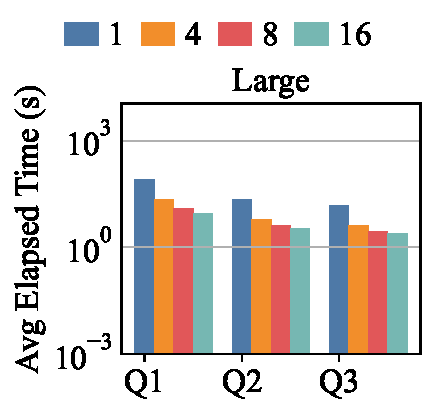
\includegraphics[scale=.6]{parts/architectures/images/query_threads_mimic.pdf}
    \caption{\textsf{MIV}}
\end{subfigure}
\begin{subfigure}[t]{.49\columnwidth}
    \centering
    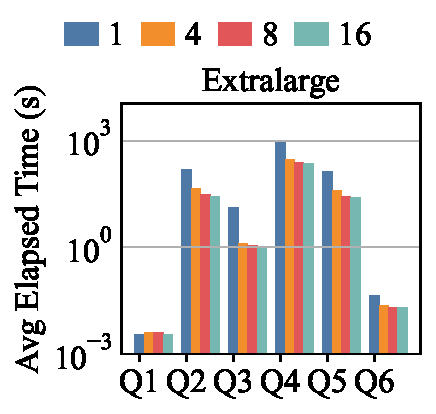
\includegraphics[scale=.6]{parts/architectures/images/query_threads_smartbench.pdf}
    \caption{\textsf{SB}}
\end{subfigure}
\caption{\#Threads speedup ($\uparrow$).}
\label{fig:opt_threads}
\end{figure}

\begin{table}[t]
\centering
\footnotesize
\caption{Average speedups.}
\label{tbl:speedups}
\begin{subtable}[t]{0.52\columnwidth}
\centering
\caption{\#Threads speedup ($\uparrow$).}
\label{tbl:opt_threads}
\setlength{\tabcolsep}{2.5pt}
\renewcommand{\arraystretch}{0.9}
\begin{tabular}{lcccc}
\toprule
 &  & 4 & 8 & 16 \\
Dataset & Size &  &  &  \\
\midrule
\multirow[*]{3}{*}{\textsf{MIV}} & S & 3.3 & 4.2 & 4.5 \\
 & M & 3.7 & 5.5 & 6.3 \\
 & L & 4.0 & 5.8 & 7.3 \\
\midrule
\multirow[*]{4}{*}{\textsf{SB}} & S & 2.8 & 3.7 & 4.3 \\
 & M & 3.2 & 4.0 & 4.6 \\
 & L & 3.6 & 4.3 & 4.9 \\
 & XL & 3.9 & 4.8 & 5.2 \\
\bottomrule
\end{tabular}
\end{subtable}
\hfill
\begin{subtable}[t]{0.42\columnwidth}
\centering
\caption{\#Machines speedup ($\uparrow$).}
\label{tbl:opt_numMachines}
\setlength{\tabcolsep}{2.5pt}
\renewcommand{\arraystretch}{0.9}
\begin{tabular}{lccc}
\toprule
 &  & 2 & 4 \\
Dataset & Size &  &  \\
\midrule
\multirow[*]{3}{*}{\textsf{MIV}} & S & 0.8 & 0.9 \\
 & M & 1.1 & 1.2 \\
 & L & 1.3 & 1.3 \\
\midrule
\multirow[*]{4}{*}{\textsf{SB}} & S & 0.8 & 0.9 \\
 & M & 1.0 & 1.1 \\
 & L & 1.3 & 1.6 \\
 & XL & 1.4 & 2.2 \\
\bottomrule
\end{tabular}
\end{subtable}
\end{table}

\Cref{fig:opt_threads} and \Cref{tbl:opt_threads} summarize the average speedup by increasing the number of execution threads in GS from 1 to 4, 8, and 16.
Speedups are computed using the execution times of \textsc{QueryTSOpt} single-thread implementation (\Cref{tbl:opt_vs_naive}) as the baseline.
For each query, the speedup is calculated as $s_{dataset, size}(x)=\frac{avg_{QID}(\textup{Time with 1 thread})}{avg_{QID}(\textup{Time with x threads})}$, and the values reported in the table correspond to the average speedup across all queries for a given dataset and size.
%Bottom- and top-most speedups are dropped to manage outliers.
Results show substantial benefits from parallel execution, with speedups ranging from approximately 2.8x to 7.3x.
The largest gains are observed on the \textsf{MIV} dataset, where more time-series expose greater opportunities for parallelism.
Overall, the results demonstrate that the proposed implementation scales effectively with the number of threads and that parallelization complements the operator-level optimizations discussed previously.

\subsection{Scaling-out TS: \#Machines}

\begin{figure}[t]
\begin{subfigure}[t]{.49\columnwidth}
    \centering
    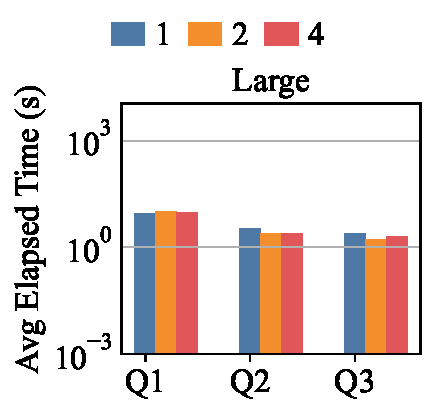
\includegraphics[scale=.7]{parts/architectures/images/query_numMachines_mimic.pdf}
    \caption{\textsf{MIV}}
\end{subfigure}
\begin{subfigure}[t]{.49\columnwidth}
    \centering
    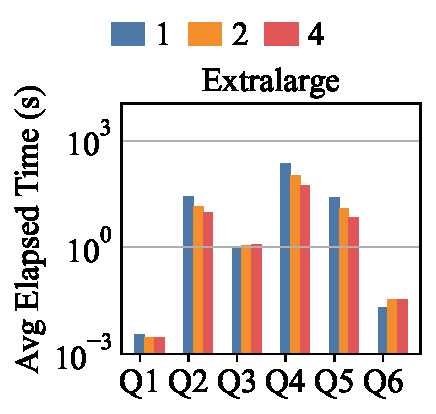
\includegraphics[scale=.7]{parts/architectures/images/query_numMachines_smartbench.pdf}
    \caption{\textsf{SB}}
\end{subfigure}
\caption{\#Machines speedup ($\uparrow$).}
\label{fig:opt_numMachines}
\end{figure}

\Cref{fig:opt_numMachines} and \Cref{tbl:opt_numMachines} summarize the average speedup by increasing the number of machines from 1 to 2 and 4.
Speedups are computed using the execution times of \textsc{QueryTSOpt} single-machine implementation (\Cref{tbl:opt_vs_naive}) as the baseline.
For each query, the speedup is calculated as $s_{dataset, size}(x)=\frac{avg_{QID}(\textup{Time with 1 machine})}{avg_{QID}(\textup{Time with x machines})}$, and the values reported in the table correspond to the average speedup across all queries for a given dataset and size.
%Bottom- and top-most speedups are dropped to manage outliers.
As expected, for small datasets using multiple machines does not provide significant benefits and may even introduce overhead, resulting in speedups less than 1.
However, as dataset size increases, the benefits of distributed execution become more evident, with speedups exceeding 1 and reaching up to 2.2x for the largest \textsf{SB} dataset.
For datasets with shorter time-series (\textsf{MIV}), the speedup from distributed execution is more modest, due to the lower computational demands and the overhead of coordination between machines.

\subsection{Comparison}
\begin{table}[t]
\centering
\footnotesize
\caption{Characteristics of SOTA approaches.}
\label{tab:related_comparisons}
\begin{tabular}{lcccccc}
\toprule
& \multicolumn{2}{c}{Expressiveness} & \multicolumn{2}{c}{Engine} & \multicolumn{2}{c}{Deployment} \\
           \cmidrule(lr){2-3}\cmidrule(lr){4-5}\cmidrule(lr){6-7}
                & Spatial     & Temporal      & Graph     & Time-series   & Distributed   & Persistent \\
\midrule
AGTS            & \ding{51} &           & \ding{51} & \ding{51}     &               & \ding{51}\\
AeonG           &           & \ding{51} & \ding{51} &               &               & \ding{51}\\
HyGraph         &           &           & \ding{51} & \ding{51}     &               &          \\
Neo4J           &           &           & \ding{51} &               &               & \ding{51}\\
\ourapproach    & \ding{51} & \ding{51} & \ding{51} & \ding{51}     & \ding{51}     & \ding{51}\\
\bottomrule
\end{tabular}
\end{table}

\ourapproach is compared against state-of-the-art approaches on temporal graphs and time-series.
\Cref{tab:related_comparisons} summarizes the functional differences among the evaluated systems in terms of spatial and temporal expressiveness, graph and time-series (native) engines, and deployment properties.
Neo4J is a single-model solution based on property graphs.
AeonG~\cite{DBLP:journals/pvldb/HouZWLJWD24} is a native solution for temporal graphs; as in Neo4J, time-series events are treated as graph nodes.
HyGraph~\cite{DBLP:conf/edbt/Ammar0BR25} is a multimodel solution that stores graph and time-series data in-memory (only).
AGTS is a multistore solution extending PostgreSQL with Apache AGE, PostGIS, and TimescaleDB; by relying on PostGIS, it is the only competitor that supports spatial queries.


The comparison is carried out with respect to (1) ingestion, (2) querying, and (3) storage footprint.
Time speedup is computed as $s_{dataset, size}(competitor)=\frac{avg_{QID}(\textup{Competitor Time})}{avg_{QID}(\textup{\ourapproach Time})}$.
$\textup{\ourapproach Time}$ refers to the values of \textsc{QueryTSOpt} in \Cref{tbl:opt_vs_naive} and the values reported in the table correspond to the average speedup across all queries for a given dataset and size.
%Bottom- and top-most speedups are dropped to manage outliers.
Speedup values $>1$ indicate that \ourapproach is faster.
To ensure a fair comparison, all solutions were evaluated under a single-threaded execution environment and average performance is obtained by aggregating twenty experimental runs.
Storage compression is computed as $c_{dataset, size}(competitor)=\frac{\textup{Competitor Storage (MB)}}{\textup{\ourapproach Storage (MB)}}$.
Compression values $>1$ indicate that \ourapproach is more compact.

\textsf{SB}-XL is omitted from the comparison since no competitor was able to load it within the allocated time. 

\subsubsection{Ingestion}

\begin{table}[t]
\centering\footnotesize
\caption{Ingestion and querying speedups with respect to competitors.
\ourapproach is faster if speedup values $>1$.}\label{tab:comparison}
\begin{subtable}[t]{\columnwidth}
\centering
\caption{Ingestion speedup ($\uparrow$).}\label{tab:comp_ing}
\begin{tabular}{lccccc}
\toprule
 &  & AGTS & AeonG & HyGraph & Neo4J \\
Dataset & Size &  &  &  &  \\
\midrule
\multirow[*]{3}{*}{\textsf{MIV}}
& S & \oot$^\dagger$ & 161.4 & 712.5 & \oot$^\dagger$ \\
& M & \oot$^\dagger$ & 184.1 & 812.8 & \oot$^\dagger$ \\
& L & \oot$^\dagger$ & \oot$^\ddagger$ & \oot$^\ddagger$ &   \oot$^\dagger$ \\
\midrule
\multirow[*]{3}{*}{\textsf{SB}}
& S & 2.4 & 241.7 & 0.4 & 64.8 \\
& M & 2.9 & 381.2 & 0.3 & \oot$^\dagger$ \\
& L & 14.9 & \oot$^\ddagger$ & \oot$^\ddagger$ & \oot$^\dagger$ \\
\bottomrule
\end{tabular}
\end{subtable}
\hfill
\begin{subtable}[t]{\columnwidth}
\centering
\caption{Query speedup ($\uparrow$).}
\label{tab:comp_query}
\begin{tabular}{lccccc}
\toprule
 &  & AGTS & AeonG & HyGraph & Neo4J \\
Dataset & Size &  &  &  &  \\
\midrule
\multirow[*]{3}{*}{\textsf{MIV}}
 & S & 2.2 & 5.7 & 9445.5 & 1.6 \\
 & M & 22.3 & 35.3 & 14205.1 & 1.7 \\
 & L & 260.0 & $\ddagger$ & $\ddagger$ & 1.7 \\
\midrule
\multirow[*]{3}{*}{\textsf{SB}}
 & S & 4.3 & 37.7 & 40.7 & 1.8 \\
 & M & 4.5 & 39.9 & 41.7 & 2.1 \\
 & L & 4.8 & $\ddagger$ & $\ddagger$ & 4.8 \\
\bottomrule
\end{tabular}
\end{subtable}
\vspace{1mm}
\footnotesize
\oot: ingestion failed or terminated because more than 500$\times$ slower than \ourapproach.\\
$\dagger$ Bulk loading was used to enable subsequent query experiments. \\
$\ddagger$ No bulk loading is available; no query results could be obtained if ingestion failed.
\end{table}

For both \textsf{MIV} and \textsf{SB}, the ingestion process involves processing a stream of events.
Each event insertion potentially includes getting the corresponding graph node and creating new nodes and edges for time-series events.

\Cref{tab:comp_ing} reports the ingestion performance.
AGTS stores graph structures on top of relational tables.
Consequently, graph insertions incur both graph-layer processing and relational storage overhead.
%, including index maintenance, tuple management, WAL logging, and transactional synchronization.
% This design is less suitable for high-throughput streaming workloads involving large volumes of temporal events.
As a result, high-frequency time-series ingestion workloads become bottlenecked by graph maintenance operations. % rather than raw data insertion throughput. 
Several ingestion attempts for AGTS and Neo4J failed to complete within a reasonable time frame, necessitating the use of bulk loading strategies that are not representative of streaming ingestion performance ($\dagger$ in \Cref{tab:comp_ing}).
AeonG triggers an update for each event insertion, which introduces additional overhead and significantly longer ingestion times; this prevented the possibility to complete the ingestion process for the larger datasets within practical limits ($\ddagger$ in \Cref{tab:comp_ing}).
Finally, while HyGraph's in-memory design allows for high throughput, it fails to scale to larger datasets due to memory constraints, resulting in out-of-memory errors for the larger datasets ($\ddagger$ in \Cref{tab:comp_ing}).

Overall, \ourapproach separates graph from time-series management, allowing events to be efficiently appended independently of graph updates.
This design substantially reduces ingestion costs for persistent baselines and improves scalability; the only speedups below 1 occur against in-memory HyGraph on small and medium \textsf{SB}, which does not provide persistence and fails at larger scales.

\subsubsection{Querying} 

\Cref{tab:comp_query} reports the query performance relative to competing systems.
On the larger datasets, AGTS and Neo4J remain the only comparable baselines among the evaluated competitors, since AeonG and HyGraph could not be queried when ingestion did not complete.
AeonG and HyGraph achieve similar performance in \textsf{SB}, but managing \textsf{MIV} substantially decreases HyGraph performance.
Among the completed runs, \ourapproach maintains a clear advantage over all competitors, with speedups generally increasing as dataset size grows.

\ourapproach becomes increasingly advantageous as dataset size and time-series cardinality grow and is the only system that consistently remains competitive across graph-time-series workloads, demonstrating the effectiveness of its hybrid architecture in combining graph navigation capabilities with efficient temporal data processing.

\subsubsection{Data compression and storage footprint}

\begin{table}[t]
\centering
\footnotesize
\caption{Storage footprint and compression.}
\label{tab:compression}

\begin{subtable}[t]{\columnwidth}
\centering
\caption{
Physical storage footprint of \ourapproach.
GS statistics include only materialized nodes and edges, while TS statistics include time-series events.
Virtual edges (i.e., edges connecting graph nodes and events) are exposed at query time but are not materialized.
Events dominate the logical data volume and storage footprint.
}\label{tab:compression-stgraph}

\resizebox{\columnwidth}{!}{%
\begin{tabular}{lccccccc}
\toprule
& & \multicolumn{3}{c}{GS} & \multicolumn{2}{c}{TS} & \\
\cmidrule(lr){3-5}
\cmidrule(lr){6-7}
Dataset & Size & \#Nodes & \#Edges & Size (MB) & \#Events & Size (MB) & Total (MB) \\
\midrule
\multirow{3}{*}{\textsf{MIV}}& S & $1.3\cdot10^3$ & $6.2\cdot10^2$ & 7.4 &
$1.7\cdot10^6$ & 70 & 77 \\
& M & $1.3\cdot10^4$ & $6.6\cdot10^3$ & 74 &
$1.7\cdot10^7$ & 698 & 772 \\
& L & $1.3\cdot10^5$ & $6.5\cdot10^4$ & 734 &
$1.7\cdot10^8$ & 6949 & 7683 \\
\midrule
\multirow{4}{*}{\textsf{SB}}& S & $3.4\cdot10^{3}$ & $6.7\cdot10^{3}$ & 2.1 &
$2.5\cdot10^{6}$ & 60 & 62 \\
& M & $6.0\cdot10^{3}$ & $1.2\cdot10^{4}$ & 4.6 &
$1.0\cdot10^{7}$ & 234 & 239 \\
& L & $2.6\cdot10^{4}$ & $5.5\cdot10^{4}$ & 16 &
$2.6\cdot10^{8}$ & 5795 & 5811 \\
& XL & $6.0\cdot10^{3}$ & $1.2\cdot10^{4}$ & 4.6 &
$3.0\cdot10^{8}$ & 6332 & 6336 \\
\bottomrule
\end{tabular}}
\end{subtable}

\begin{subtable}[t]{\columnwidth}
\centering
\caption{Compression with respect to competitors.
\ourapproach is more compact if compression values $>1$.}
\label{tab:compression-competitors}
\begin{tabular}{lccccc}
\toprule
Dataset & Size & AGTS & AeonG & HyGraph & Neo4J \\
\midrule
\multirow{3}{*}{\textsf{MIV}}
 & S & 2.4 & 7.6 & $\dagger$ & 4.2 \\
 & M & 2.4 & 7.6 & $\dagger$ & 4.4 \\
 & L & 2.4 & $\ddagger$ & $\ddagger$ & 4.3 \\
\midrule
\multirow{3}{*}{\textsf{SB}}
 & S & 10.8 & 9.4 & $\dagger$ & 7.8 \\
 & M & 10.9 & 8.4 & $\dagger$ & 7.5 \\
 & L & 11.5 & $\ddagger$ & $\ddagger$ & 7.5 \\
\bottomrule
\end{tabular}
\\
$\dagger$ In-memory. \\
$\ddagger$ No bulk loading is available; no data was stored (see \Cref{tab:comparison}).
\end{subtable}
\end{table}

\ourapproach does not materialize edges toward individual events; instead, events are accessed through virtual edges that are generated at query time.
As the number and length of time-series increase, this significantly reduces storage footprint.
\Cref{tab:compression-stgraph} shows the effectiveness of the hybrid storage layout and the physical separation between graph and time-series data.
Storage grows approximately linearly with the number of temporal events: for instance, in the MIV dataset, increasing the event count from $1.7\cdot10^6$ to $1.7\cdot10^8$ results in a growth from 77 MB to 7.7 GB. 
The time-series storage (TS) dominates the overall footprint, accounting for more than 90\% of the total space in all datasets, while the graph structure (GS) remains comparatively small.
When compared to the original datasets (\Cref{tab:datasets}), \ourapproach saves up to $10^4$ times in terms of stored edges.

\Cref{tab:compression-competitors} reports the compression ratio with respect to competitors and it shows that \ourapproach remains substantially more compact than alternative systems, achieving compression factors between $2.4\times$ and $11.5\times$.
The largest gains are observed on the SB datasets, where \ourapproach requires up to an order of magnitude less space than AGTS, AeonG, and Neo4J.
Furthermore, several large instances cannot be managed by AeonG or HyGraph.

\section{Conclusion and future directions}\label{sec:conclusion}

This paper introduced \ourapproach, a multistore system for managing spatio-temporal property graphs whose data combine slowly evolving graph structures with high-volume time-series.
\ourapproach exposes a unifying spatio-temporal property graph abstraction while physically separating graph nodes and edges, stored in GS, from time-series events, stored in TS.
The connection between the two stores is provided at query time through virtual edges, avoiding the materialization of one graph edge per event.
\ourapproach supports temporal validity for nodes, edges, and properties, and rewrites query plans so that event-local operators can be pushed down to TS.
The experimental evaluation shows that this design reduces storage overhead, improves ingestion, and accelerates analytical queries with respect to single- and multimodel and multistore baselines.

Several research directions remain open.
\ourapproach 
(i) currently supports conjunctive path queries, adding regular path queries would enable more expressive graph navigation while introducing new opportunities for cross-store optimization;
(ii) follows the property-graph paradigm, enriching it with native time-series operators would allow users to combine graph traversal and temporal analytics within a unified model;
(iii) currently optimizes single-access time-series queries, a global optimizer capable of jointly reasoning about multiple time-series operations could further improve execution efficiency;
(iv) targets historical queries, supporting streaming graph-time-series workloads would enable real-time monitoring and decision-making over continuously evolving data.


\begin{partsummary}

This part addressed the first two steps of the progression outlined at the close of \Cref{chap:data_oriented_perspective}: proposing a general-purpose schema for the data architecture of a Digital Twin, and proposing a data model, and a consequent system to manage, integrate and represent Digital Twin data.

\Cref{chap:dataplat} addressed the first step, through the design of a data platform for the AGRITECH precision agriculture case study. The requirements identified there, arising directly from the volume, variety, velocity, and veracity of the data produced by six independently developed research activities, motivated a reference architecture organized around independent, composable modules -- ingestion, storage, data processes, management, and exploitation -- together with a domain-level conceptual schema generalizing the entities recurring across these activities into agents, environments, measurements, and tasks. \Cref{chap:datamodel-dt} addressed the second step, showing that implementing this conceptual schema relationally exposes two difficulties characteristic of Digital Twin data more generally: the dynamic, time-varying relationships among entities, which relational schemas can only represent through proliferating association tables, and the rigidity such schemas impose on later extension. STGraph, the multistore system presented in that chapter, addressed both difficulties by representing entities and their evolving relationships as a spatio-temporal property graph, while delegating the high-volume time-series data such entities produce to a dedicated time-series store connected to the graph through virtual edges.

Once a Digital Twin's data is integrated and represented through this reconciled layer, it becomes possible to explore the functionality such integration newly enables; \Cref{part:methods-applications} does so directly, illustrating applications built on top of the platform and data model presented in this part. At the same time, the growing complexity of these data representations, and of the infrastructure required to support them, raises a complementary question: how such complexity can be managed, and made tractable for the humans who must still interact with it. \Cref{part:methods-applications} also explores methods addressing this question, aimed at easing human interaction with increasingly complex data representations and the systems built around them.

\end{partsummary}

%%%%%%%%%%%%%%%%%%%%%%%%%%%
%%%%%%%%%%%%%%%%%%%%%%%%%%%

\part{Methods and Applications}
\label{part:methods-applications}
\chapter{Methods}
\label{chap:methods}
{\color{red}
\Cref{chap:dataplat} introduced a reference architecture for domain-level data platforms, organized around a small set of composable modules -- ingestion, storage, data processes, management, and exploitation -- and distinguished, within the data processes module, between platform processes, maintained by the platform itself, and user processes, the application-specific pipelines through which individual Digital Twins consume and produce data. That architecture, however, is deliberately abstract: it specifies which functionalities a data platform must provide, not which concrete technology should implement each of them. In practice, cloud providers such as Amazon, Google, and Microsoft expose ecosystems of dozens of overlapping, interoperable services, and selecting the right subset for a given application is, in current practice, left to the expertise of individual designers or consultants -- an unstructured, largely non-reproducible process, at odds with the standardization this thesis has argued for throughout.

This chapter addresses this gap, presenting a methodology that systematizes the selection of the concrete services instantiating the modules of a data platform, driven directly by the data-intensive processes the platform is meant to support. In terms of the platform/user process distinction introduced in \Cref{sec:dataplat-refarch}, the methodology takes as input a description of an application's user processes -- for a Digital Twin, its own analytical or operational data pipelines -- and derives, systematically rather than by expert intuition alone, the subset of services from a given ecosystem that implements them at minimal cost, while respecting dependency, compatibility, and mandatory constraints the designer may impose. Fittingly, the resulting characterization of a data platform is the same one adopted throughout this thesis (\Cref{chap:data_oriented_perspective}): a centralized infrastructure providing independent and composable services meeting the end-to-end needs of data pipelines.
}

\section{Data as a blueprint - Process driven design of Data Platforms}
\label{sec:process-driven-design}



Data platforms are state-of-the-art solutions to implement data-driven applications and analytics, since they facilitate the ingestion, storage, management, and exploitation of big data. Data platforms are built on top of complex ecosystems of services answering different data needs and requirements; such ecosystems are offered by different providers (e.g., Amazon AWS and Microsoft Azure). However, when it comes to engineering data platforms, no unifying strategy and methodology is available yet, and the design is mainly left to the expertise of practitioners in the field. Service providers simply expose a long list of interoperable and alternative engines, making it hard to select the optimal subset without a deep knowledge of the ecosystem. A more effective approach to the design starts from the knowledge of the data transformation and exploitation processes that should be supported by the platform. We sketch a computer-aided design methodology and then focus on the selection of the optimal services needed to implement such processes. We show that our approach lightens the design of data platforms and enables an unbiased selection and comparison of solutions even through different service ecosystems.

\subsection{Introduction}

Digital transformation is one of the most disruptive trends of recent years. Digitization is perceived as the most effective solution to innovate every industrial sector thanks to process automation and the (automatic) exploitation of the value hidden in data. Such evolution is pushing information systems towards complex ecosystems of data-oriented services answering different data needs and requirements.

{\color{red}As already characterized in \Cref{chap:data_oriented_perspective}, }a data platform is a centralized infrastructure that facilitates the ingestion, storage, management, and exploitation of large volumes of heterogeneous data. It provides a collection of independent and composable services meeting the end-to-end needs of data pipelines, where: \textit{centralized} means that a data platform is conceptually a single and unified component; \textit{independent} means that changes in the implementation of a service do not affect other services; \textit{composable} means that services have interfaces that enable an easy and frictionless composition; and \textit{end-to-end} means that services cover the entire data life cycle. Data platforms foster collaboration and shared governance (being centralized, data is unified following some integration and it is easier to ensure compliance with data protection and privacy laws through shared security and access control), and scalability (being implemented on a distributed infrastructure, it is easy to add storage and computing resources as needed).

When it comes to building data platforms, no unifying strategy and methodology is there yet: building data platforms is mainly left to the expertise of practitioners or consultancy companies. On the one hand, cloud service providers\footnote{While data platforms are not mandatorily coupled with cloud computing, cloud computing is proving to be a winning business model since deploying and maintaining such a variety of computational resources and assets requires advanced technical skills that companies hardly have ``in-house''.} offer ecosystems of services composed of many engines interoperable with each other; however, choosing the optimal set of services is hard since multiple solutions could fulfill the desiderata (e.g., whether disjoint databases and data warehouses or a single Lakehouse \cite{DBLP:conf/cidr/Zaharia0XA21} should be used) and could require vertical knowledge on the design of data pipelines. On the other hand, several abstract big data architectures have been introduced (e.g., NIST \cite{chang2019nist}, Lambda \cite{DBLP:conf/bigdataconf/KiranMMDB15}, and Kappa \cite{kreps2014questioning}). However, while they provide the necessary functionalities to enable big-data applications, their implementation and adoption require to understand which services should be used.

Neither providers of service ecosystems nor abstract architectures answer a crucial question: \textit{given an ecosystem of services and the data-driven processes to support, which is the optimal subset of services enabling such processes?} Answering this question is hard since (i) each provider offers many (overlapping) services, (ii) different providers offer different service categorizations that can hardly be mapped together, (iii) the evolution of cloud ecosystems is fast and stakeholders without vertical technical knowledge can hardly keep up with the pace, and (iv) simply selecting ``all'' engines is not viable due to cost and management reasons. We believe that to ease the data platform design, the description of data-driven processes should drive such activity. Indeed, data pipelines are the backbone of a \textit{data} platform as they determine information-rich representations, and are congenial to designers since they encode many constraints on the choices to be made.

This chapter introduces the following contributions.
\begin{itemize}
    \item A methodology to guide the selection of blueprints for (cloud) data platforms driven by clients' processes.
    \item The formulation of such selection as an optimization problem where preferences, affinity, and further constraints can be applied.
    \item The discovery of (architectural) design patterns in clients' processes to align the blueprint with well-known solutions.
    \item Extraction of blueprints from real case studies and validation with experts from consultancy companies.
\end{itemize}
This work extends the methodology described in \cite{DBLP:conf/dolap/FranciaGP24} and introduces these novelties: (i) management of advanced design patterns such as Lakehouse to replace both data lakes and warehouse; (ii) extension of the matching and selection steps to support and select such advanced patterns depending on their requirements; and (iii) discussion and comparison of two additional (real) case studies assessed by consultants from two Italian companies using two different service providers.

{\color{red}The remainder of this chapter is organized as follows.} \Cref{sec:pdd-overview} sketches the overall methodology; \Cref{sec:pdd-case} describes the case studies used in the chapter; \Cref{sec:pdd-eco} and \Cref{sec:pdd-process} describe and formalize the design steps; \Cref{sec:pdd-patterns} introduces the match and selection of design patterns; \Cref{sec:pdd-eval} evaluates the effectiveness and efficiency of the contribution; and \Cref{sec:pdd-related} analyzes the related literature. Finally, \Cref{sec:pdd-conclusion} draws the conclusions and future directions.

\subsection{Methodology Overview}
\label{sec:pdd-overview}

\begin{figure}[htbp]
    \centering
    %[FIGURE: overview della metodologia -- 5 blocchi/frecce: (1) service ecosystem, (2) DFD requirements, (3) tag enrichment, (4) match, (5) augment, (6) optimize]
    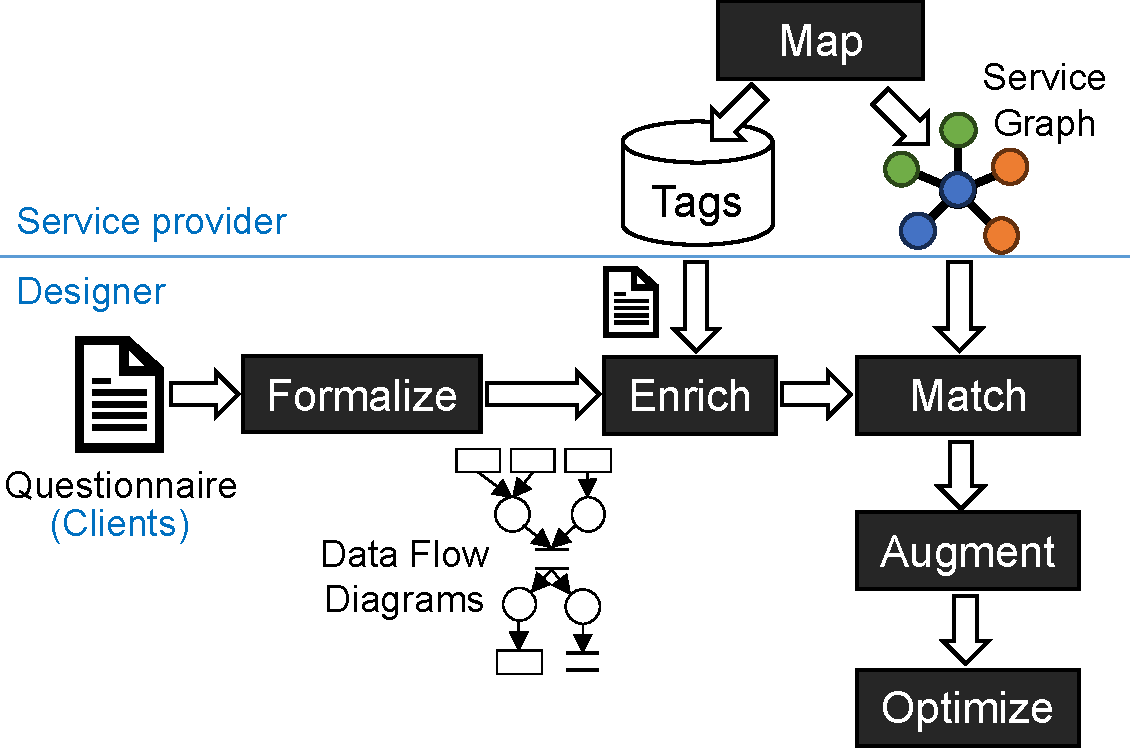
\includegraphics[width=0.8\textwidth]{parts/methods/images/overview.pdf}
    \caption{Overview of the methodology.}
    \label{fig:pdd-overview}
\end{figure}

Engineering a data platform is nontrivial. A data platform must be designed upon a principle of modularity to be extensible with new components and functionalities. While it is true that reference architectures exist (as later discussed in \Cref{sec:pdd-related}), not all their modules and services might be necessary. Indeed, running useless functionalities and services results in a waste of resources and money (e.g., in cloud environments where users pay for the running time of the allocated resources).

To effectively build a data platform, we propose a methodology (\Cref{fig:pdd-overview}) that involves three types of users: \emph{cloud service providers} (IT experts with in-depth knowledge of services available in the ecosystem); data platform \emph{designers} (consultants or people with expertise in designing data flows but with no vertical knowledge on cloud/service ecosystems) and \emph{clients} asking for the design of the data platform blueprint (e.g., partners involved in the same European project with expertise on the applicative domain ---such as precision agriculture--- but no expertise on IT and architectures). {\color{red}In the setting of this thesis, a client corresponds to the developer of a Digital Twin's user process (\Cref{sec:dataplat-refarch}): someone with expertise in the physical process or application domain the Digital Twin represents, but not necessarily in the underlying data infrastructure.}

The methodology aims to assist designers in selecting the services necessary to implement the clients' data pipelines out of the ``unstructured'' lists of services provided by cloud providers.

Here, we sketch the five steps composing the methodology, and we mainly focus on steps (4), (5), and (6) in the remainder of the chapter.

\paragraph{(1) Define the service ecosystem.}
A cloud service provider identifies \textit{una tantum}: (i) the alternative candidate services to compose the blueprints of data platforms, and (ii) a taxonomy of tags that describe and characterize such services. The identified services are organized in a service graph describing the preferences and relationships between them as well as the tags characterizing each service.

Assuming that cloud service providers do not offer redundant services, our guideline for designing the tag taxonomy emphasizes ensuring sufficient expressiveness. This means that each service should be uniquely identifiable by a set of tags.

\begin{example}
Within the Amazon Web Services (AWS) ecosystem, there are several services for managing relational data but they have different purposes. For instance, RDS is used to manage operational workloads while Redshift is used to manage data warehouses and OLAP workloads. To distinguish these two services, the tag taxonomy should be expressive enough (i.e., have enough tags) so that RDS and Redshift differ for at least one tag.
\end{example}

\paragraph{(2) Formalize the requirements through a Data Flow Diagram.}
When building the blueprint of a new data platform, clients compile questionnaires that collect information about their data-driven processes and the main steps, subjects, and goals of their analysis. Note that the data platform should support (possibly independent) processes from multiple clients.

Designers then refine the answers to the questionnaires and formalize the processes into a Data Flow Diagram (DFD); during the process, a few interviews with the clients might be necessary. We choose the DFD formalism \cite{DeMarco78} since it represents flows of data through an information system at a high level of abstraction, emphasizing the movement and transformation of data while hiding details such as decision points and interactions: knowing which repositories and processes compose the data-driven processes is enough to return a blueprint.

To build the DFD, designers decompose the data flows into agents, processes, and repositories. Starting from an aggregated overview, our guideline is to recursively split candidate processes and repositories until each of them is characterized by homogeneous tags (e.g., if a repository contains both unstructured images and relational tables, split it into two homogeneous repositories). Repositories and processes that should not be imported into the data platform (e.g., legacy systems deployed on-premises) should be treated as external agents.

\paragraph{(3) Enrich the DFD with service tags.}
To match the DFD with the services deployed in a cloud ecosystem, the two must share the same characterization. Each process and repository in the DFD is enriched with the tags from the taxonomies previously identified by the cloud service provider. To aid designers in the characterization of each process/repository (agents are not subjects of enrichment, since they are out of the scope of the platform), clients answer an additional set of questions; we recall that clients are not required to have vertical knowledge about computer and data science or engineering. Such questions are defined by the cloud service providers and driven by the tag taxonomies. Note that since our final goal is selecting the most appropriate services, we are not interested in identifying and tracking the data/processes but rather their types and their flows.

\begin{example}
Given a repository from the DFD, we ask the question: ``What are the main types of collected data?'' -- Sensor data, Images, Videos, Satellite observations, \textbf{Tables}. Answering ``Satellite observations'' tags the repository with the properties \prop{Volume}{Big}, \prop{Data Model}{File}, and \prop{Data Nature}{Raster} since earth observations are data-heavy files (e.g., around 1 GB for 100 $km^2$) and tags the process to download such data as \prop{Collection}{Pull} since files are downloaded from an FTP server \cite{esa-eo}.
\end{example}

\paragraph{(4) Match the DFD and service graphs.}
Once the DFD and service graphs are characterized by tags from the same taxonomies, it is possible to join them in a matched graph. A DFD process or repository matches (i.e., can be implemented by) a service only if the service has the same or more functionalities to fully implement it.

\paragraph{(5) Augment the matched graph.}
Augmentation is a semi-automatic step atop the matched graph. On the one hand, the system automatically recognizes architectural design patterns in the data pipelines to either automatically apply or simply highlight advanced compositions of services. On the other hand, designers can manually inject their knowledge to enrich the matched graph and steer the subsequent optimization. Designers could force the selection of services in case they are required by clients, prefer some services in place of others for performance or compatibility reasons, and refine the match (e.g., consider only services supporting programming languages required by legacy software).

\paragraph{(6) Select the optimal services.}
Out of all the services that are candidate implementations, it is necessary to select the minimal blueprint of the data platform that covers all the DFD entities (the fewer the services, the lower the cost and management efforts). Furthermore, dependencies and compatibilities between services have to be taken into account.

\subsection{Case Study: Agritech}
\label{sec:pdd-case}

Within the Agritech spoke of the NRRP European project \cite{pnrr}, we deploy a data platform supporting prescriptive analytic tasks from 8 clients in the field of precision agriculture.\footnote{{\color{red}This figure refers to the client base considered for the process-driven design methodology; \Cref{chap:dataplat} discusses the same Spoke~3 initiative with reference to its 6 formal research partners. The two counts are not necessarily inconsistent (e.g., industrial use cases versus partner institutions), but have not been independently reconciled for this thesis.}} We will use one of the partners as a working case study throughout the chapter. Here follows a qualitative description of one of the clients' data flows that the platform must support.

\begin{example}
\label{ex:pdd-qgen}
The analysis entails a flow that is structured as follows. (i) Data comes from soil moisture sensor grids, weather stations, and SENTINEL-2 satellites; (ii) Sensor and weather data is uploaded every 15 minutes to the platform, while satellite data is periodically downloaded; (iii) Soil moisture data is interpolated using mathematical (e.g., bilinear interpolation) and machine learning (e.g., neural networks) techniques; (iv) Vegetation indexes are computed out of the raw satellite observations and integrated with the enriched sensor data; (v) Reports are periodically generated out of the integrated data; (vi) Given an optimal soil moisture matrix, the integrated data is used to decide how much to irrigate the soil.
\end{example}

\begin{figure}[htbp]
    \centering
    %[FIGURE: DFD dell'esempio -- Moisture Sensors/Weather Stations -> Consume -> Sensor Data; Satellite -> Download -> Raw Images; Sensor Data -> Enrich -> Integrated Data; Raw Images -> vegetation index -> Integrated Data; Integrated Data -> ETL -> Data Warehouse; Irrigation Optimization -> Field Valves]
    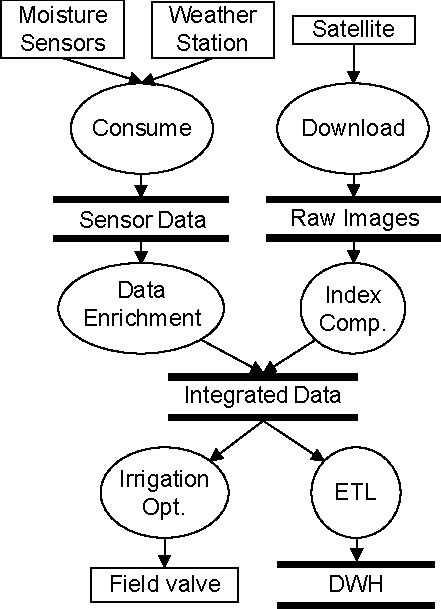
\includegraphics[width=0.4\textwidth]{parts/methods/images/dfd.pdf}
    \caption{DFD from \Cref{ex:pdd-qgen}.}
    \label{fig:pdd-dfd}
\end{figure}

After gathering questionnaires from the clients, we (designers) iteratively refined the interview into a DFD.
\begin{example}[DFD]
\Cref{fig:pdd-dfd} depicts the tasks from \Cref{ex:pdd-qgen} using the DFD formalism.
\begin{itemize}
    \item \dfd{Moisture Sensors} and \dfd{Weather Stations} stream data into the platform, such data is \dfd{Consume}d and stored in the original format into \dfd{Sensor Data};
    \item \dfd{Satellite} images are periodically \dfd{Download}ed and stored into \dfd{Raw Images};
    \item \dfd{Sensor Data} are \dfd{Enrich}ed, interpolated, and stored into \dfd{Integrated Data};
    \item \dfd{Raw Image}s are used for the computation of vegetation indexes and integrated with sensor data;
    \item \dfd{Integrated Data} are used to fuel a \dfd{Data Warehouse} through \dfd{ETL};
    \item The \dfd{Irrigation Optimization} algorithm controls the \dfd{Field Valve}s installed in Emilia Romagna, Italy.
\end{itemize}
Following the guidelines, the data collection processes cannot be merged into a single one since (i) \dfd{Moisture Sensors} streams data into the platform while \dfd{Satellite} images are periodically downloaded, and (ii) \dfd{Sensor Data} and \dfd{Raw Images} cannot be grouped into a single repository since they contain heterogeneous data types. More details on such tasks are described in \cite{DBLP:journals/cea/FranciaGG22,baldi2023smart}.
\end{example}

\subsection{Mapping the Service Ecosystem}
\label{sec:pdd-eco}

Tags (\Cref{tab:pdd-tags}) are organized as a collection of hierarchies that can be fueled bottom-up from the documentation of cloud services providers (i.e., the set of tags that are attached to each service or that are inferrable through the service description), and top-down from the literature; for instance, the big data V's \cite{anuradha2015brief}, such as volume (small to big), variety (structured to unstructured), and velocity (low to high).

\begin{definition}[Hierarchy]
A \emph{hierarchy} $h$ is a taxonomy of categorical values $Dom(h)$. $\geq_{h}$ is the partial order that defines the taxonomy; $\geq_{h}$ indicates whether a value is more specific than another. We denote with $H$ the set of hierarchies.
\end{definition}

\begin{example}[Tags and hierarchies]
\Cref{tab:pdd-tags} depicts an example of hierarchies $H=\{\sf{Data Model}, \sf{Volume}, ...\}$. In the partial order of the hierarchy $h=\sf{Data Model}$ it is, for instance, $\textup{Relational}\geq_{\sf{Data Model}} \textup{Structured} \geq_{\sf{Data Model}} \textup{Data Model (All)}$. $\textup{Relational}$ is more specific than $\textup{Structured}$ in the \sf{Data Model} hierarchy.
\end{example}

\begin{table}[!ht]
\centering
\scriptsize
\caption{Examples of taxonomies of tags.}
\label{tab:pdd-tags}
\begin{tabular}{lll}
Data Model (All)        & Structured            & Relational\\\cline{3-3}
                        &                       & Multidimensional\\\cline{2-3}
                        & Semi-structured       & Document\\\cline{3-3}
                        &                       & Wide-column\\\cline{2-3}
                        & Unstructured          & Key-value\\\cline{3-3}
                        &                       & Graph\\\cline{3-3}
                        &                       & File (text, binary)\\\cline{1-3}
&&\\
Data Nature (All)       & Spatial               & Vectorial\\\cline{3-3}
                        &                       & Raster\\\cline{2-3}
                        & Temporal              & \\\cline{1-2}
&&\\
Volume (All)            & Small                 & \\\cline{2-2}
                        & Big                   & \\\cline{1-2}
&&\\
Data Zones (All)   & Landing               & \\\cline{2-2}
                        & Archive               & \\\cline{2-2}
                        & Processed             & \\\cline{1-2}
&&\\
Functionality (All)& ETL                   & \\\cline{2-2}
                        & Reporting        & \\\cline{2-2}
                        & Operational           & \\\cline{2-3}
                        & Machine learning      & Classification\\\cline{3-3}
                        &                       & Regression\\\cline{1-3}
&&\\
Collection (All)        & Pull                  & Cumulative\\\cline{3-3}
                        &                       & Delta\\\cline{2-3}
                        & Push                  & \\\cline{1-2}
&&\\
Computing (All)         & Batch                 & \\\cline{2-2}
                        & Mini-batch            & \\\cline{2-2}
                        & Streaming             & \\\cline{1-2}
&&\\
Language (All)          & Low code              & \\\cline{2-2}
                        & Python                & \\\cline{2-2}
                        & Java                  & \\\cline{2-2}
                        & SQL                   & \\\cline{1-2}
\end{tabular}%
\end{table}%

\begin{table}[htbp]
  \centering
  \scriptsize
  \caption{An excerpt of services from the Amazon AWS ecosystem (from \url{https://aws.amazon.com/big-data/datalakes-and-analytics}).}
  \label{tab:pdd-awsserv}
    \begin{tabular}{lp{4cm}p{4cm}}
    \toprule
    Solution areas & Use cases & AWS services \\
    \midrule
    Advanced analytics & Interactive analytics & Athena \\
          & Big data processing & EMR \\
          & Data warehousing & Redshift \\
          & Real-time analytics & Managed Service for Apache Flink \\
          & Operational analytics & OpenSearch Service \\
          & Dashboards and visualizations & QuickSight \\
          & Visual data preparation & Glue DataBrew \\
    Data management & Real-time data movement & Managed Streaming for Apache Kafka, Kinesis Data Streams, Glue \\
          & Data governance & DataZone, Glue, Entity Resolution, Lake Formation, S3 \\
          & Object storage for data lakes & S3, Lake Formation \\
          & Backup and archive for data lakes & S3 Glacier, Backup \\
          & Data catalog & Glue, Lake Formation \\
          & Third-party data & Data Exchange, Clean Rooms \\
    Machine learning & Frameworks and interfaces & Deep Learning AMIs \\
          & Platform services & SageMaker \\
    \bottomrule
    \end{tabular}%
\end{table}%

The services available on a specific ecosystem differ for each provider, and no single and shared organization of services is available. \Cref{tab:pdd-awsserv} shows an example of services from the AWS website (as of November 2023).

While a plethora of services is available, there is no necessity to consider all of them at once. Indeed, the considered services must cover the ``core'' functionalities necessary to run a data platform such as the ones proposed by NIST \cite{chang2019nist}, among them storage and data processing engines.

Also, it is necessary to consider the relationships between services (e.g., whether the adoption of a service requires another) and preferences in their choice (e.g., due to differences in performance reasons). That is why we map the services into a directed property graph.

\begin{definition}[Directed property graph]
\label{def:pdd-graph}
A \emph{directed property graph} is a tuple $G = (N, A, P, L)$ where $N=\{..., n_i, ...\}$ is a finite set of \emph{nodes}, $A=\{..., a_{ij}, ...\}$ is a finite set of \emph{arcs} connecting nodes $n_i$ and $n_j$, $P=\{..., (h, v), ...\}$ is a set of key-value \emph{properties} with $h \in H$ and $v \in Dom(h)$, and $L$ is a set of \emph{labels}. $props: (N \cup A) \rightarrow P$ returns the properties of a node or arc. $label: (N \cup A) \rightarrow L$ returns the labels of a node or arc.
\end{definition}

\begin{definition}[Path]
Given a directed property graph $G$, a \emph{path} $p_{ij}$ from node $n_i$ to node $n_j$ is a sequence of distinct arcs $(a^1_{ix}, ..., a^k_{xy}, ..., a^{|p|}_{yj})$ for which there is a sequence of distinct nodes $(n^1_{i}, ..., n^k_{x}, n^{k+1}_{y}, ..., n^{|p|+1}_{j})$ such that the arc $a^k$ connects the node $n^k$ to the node $n^{k+1}$ for $k \in [1, |p|]$. We denote with $p_{ij}.nodes$ the sequence of nodes connected by the path.
\end{definition}

\begin{figure}[htbp]
    \centering
    %[FIGURE: excerpt di service graph -- nodi S3, GeoServer, EC2, EMR, Lakehouse con archi Requires/IsCompatible e relative property]
    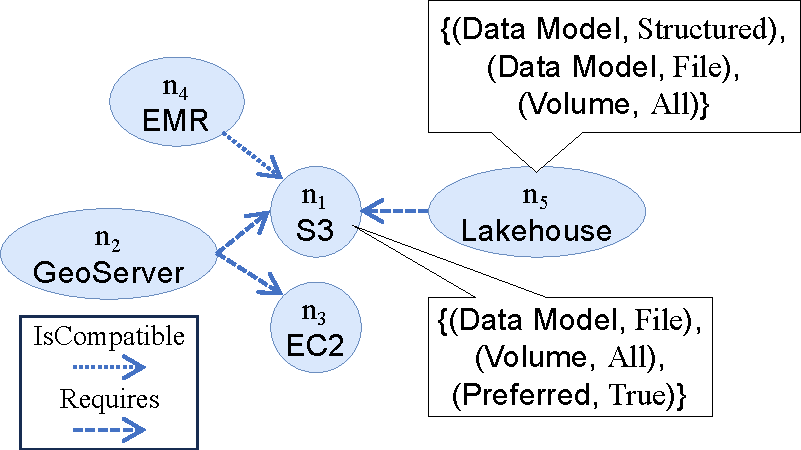
\includegraphics[width=0.7\textwidth]{parts/methods/images/servicegraph.pdf}
    \caption{Excerpt of a service graph and its properties.}
    \label{fig:pdd-servicegraph}
\end{figure}

\begin{definition}[Service graph]
\label{def:pdd-serv}
A \emph{service graph} is a directed property graph $G^S$ where nodes are labeled as \lbl{Service}, while arcs are alternatively labeled as $\{\lbl{Requires}, \lbl{IsCompatible}, \lbl{IsAkin}\}$.
\end{definition}

The semantics of the labels is the following:
\begin{itemize}
    \item \lbl{Service}: is any engine from the service ecosystem that can be optionally tagged with the property \prop{Preferred}{True} to specify whether it should be considered more than others;
    \item \lbl{Requires}: represents whether a service mandatorily relies on another;
    \item \lbl{IsCompatible}: represents whether a service natively interfaces with another (i.e., their interaction is supported by default and does not require custom/additional libraries or connectors);
    \item \lbl{IsAkin}: represents whether a service not only is compatible with another but also if their adoption together is encouraged.
\end{itemize}

\begin{example}[Service graph]
Here follows an excerpt of the service graph $G^S$ and properties built out of \Cref{tab:pdd-awsserv} and depicted in \Cref{fig:pdd-servicegraph}.
\begin{align*}
&N = \{n_1, n_2, n_3, n_4, n_5,...\}, ~
A =\{a_{23}, a_{34}, ...\}\\
&n_1 = \serv{S3},~n_2=\serv{GeoServer},~n_3=\serv{EC2},~n_4=\serv{EMR}
,~n_5 = \serv{Lakehouse}
\\
&label(n_1) = \lbl{Service}\\
&label(a_{23}) = \lbl{Requires}\\
&label(a_{41}) = \lbl{IsCompatible}\\
&props(n_1) = \{\prop{Data Model}{File},\prop{Volume}{All}, \prop{Preferred}{True}\}\\
&props(n_2) = \{\prop{Data Model}{File},\prop{Data Nature}{Raster}\}\\
&
props(n_5)=\{\prop{Data Model}{Structured},\prop{Data Model}{File},\prop{Volume}{All}\}
\end{align*}
\serv{GeoServer} requires \serv{EC2} since it is deployed on it, \serv{EMR} is compatible with \serv{S3} since it can natively read from and write to the object storage.
\end{example}

\subsection{Process-Driven Match, Augmentation, and Optimization}
\label{sec:pdd-process}

We now describe three steps composing our approach. \textit{Match} extracts the services that can support the execution of the data pipeline, \textit{Augment} refines the potential candidates and, finally, \textit{Optimize} picks the optimal (minimal) subset. We mainly focus on the optimization of the platform design rather than on how, starting from questionnaires, designers refine the DFD of such flows.

Since data pipelines are the backbone of data platforms, everything starts from the DFD describing the processes of clients' analysis.

\begin{definition}[Data Flow Diagram]
\label{def:pdd-dfd}
A \emph{Data Flow Diagram} (DFD) is a directed property graph $G^D$ where nodes are alternatively labeled as $\{\lbl{Agent}, \lbl{Repository}, \lbl{Process}\}$, while arcs are labeled as \lbl{Flow}. Arcs must connect with at least one node with label \lbl{Process}. The semantics of the labels is the following:
\begin{itemize}
    \item \lbl{Agent}: an external entity that communicates with the system and stands outside of the system;
    \item \lbl{Process}: transform inputs to outputs;
    \item \lbl{Repository}: store data for later use;
    \item \lbl{Flow}: transfer data from one part of the system to another.
\end{itemize}
\end{definition}

We recall that the DFD is enriched with tags identified by the cloud service provider (\Cref{tab:pdd-tags}).

\begin{figure}[htbp]
    \centering
    %[FIGURE: excerpt di property del DFD -- nodo Consume (Process) con archi verso Sensor Data (Relational) e Raw Images (File, Raster)]
    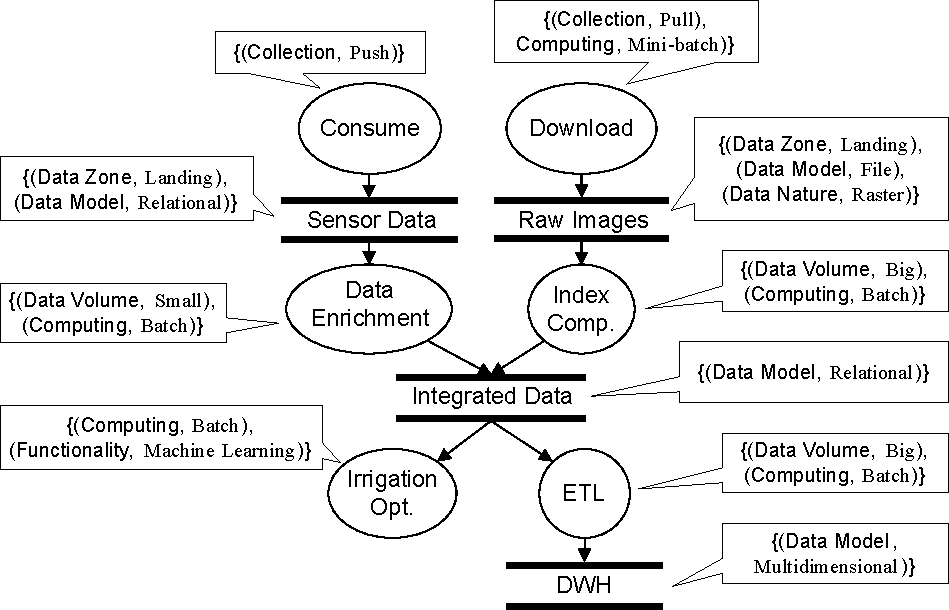
\includegraphics[width=0.8\textwidth]{parts/methods/images/dfd-ext.pdf}
    \caption{An excerpt of properties of the DFD from \Cref{fig:pdd-dfd}.}
    \label{fig:pdd-dfd-ext}
\end{figure}

\begin{example}[DFD]
Here follows an excerpt of the DFD $G^D$ and properties from \Cref{fig:pdd-dfd-ext}.
\begin{align*}
&N = \{n_1, n_2, n_3, ...\},~A =\{a_{12}, ...\}\\
&n_1 = \dfd{Consume},~n_2=\dfd{Sensor Data},~n_3=\dfd{Raw Images}\\
&label(n_1)= \lbl{Process},~label(n_2)= \lbl{Repository}\\
&label(n_3)= \lbl{Repository},~label(a_{12})=\lbl{Flow}\\
&props(n_2)= \{\prop{Data Model}{Relational}\}\\
&props(n_3)= \{\prop{Data Model}{File}, \prop{Data Nature}{Raster}\}
\end{align*}
\end{example}

\subsubsection{Matching the DFD and Service Graphs}

Given the service graph and the DFD, we can automatically join them by matching their tags.

\begin{definition}[Match]
\label{def:pdd-nodematch}
Given a DFD and a service graph, the function $match: N^D \times N^S \rightarrow \{true, false\}$ is true when, given a node $n^D \in N^D$ of the DFD and a node $n^S \in N^s$ of the service graph, each property in $props(n^D)$ matches a property in $props(n^S)$. A property $(h_i,v_i)$ matches another property $(h_j, v_j)$ if $h_i=h_j$ and $v_i \geq_{h_i} v_j$.
\end{definition}

A match represents whether a DFD node can be implemented using a specific service (solid arcs in \Cref{fig:pdd-match}); i.e., services that have the same or more generic values for the properties specified in the DFD node. For instance, a DFD repository tagged as Relational could be implemented by services supporting Relational or all Structured data.

\begin{example}[Match]
With reference to \Cref{fig:pdd-match}, given the node \dfd{Raw Images} from the DFD, and the nodes \serv{S3} and \serv{GeoServer} from the service graph
\begin{align*}
props(\dfd{Raw Images}) &= \{\prop{Data Model}{File},\prop{Data Nature}{Raster}\}\\
props(\serv{GeoServer}) &= \{\prop{Data Model}{File},\prop{Data Nature}{Raster}\}\\
props(\serv{S3}) &= \{\prop{Data Model}{File},\prop{Volume}{All}\}
\end{align*}
Since $match(\dfd{Raw Images}, \serv{GeoServer}) = true$ and $match(\dfd{Raw Images}, \serv{S3}) = false$, \dfd{Raw Images} can be implemented by \serv{GeoServer} but not directly in \serv{S3}. The former is natively capable of managing geographical data while \serv{S3} would only provide storage as plain files.
\end{example}

\begin{figure}[htbp]
    \centering
    %[FIGURE: matching tra grafo DFD (bianco) e grafo servizi (blu); in grassetto i servizi selezionati come blueprint ottimale; Athena e Churn Prediction come esempi di servizi non abbinati]
    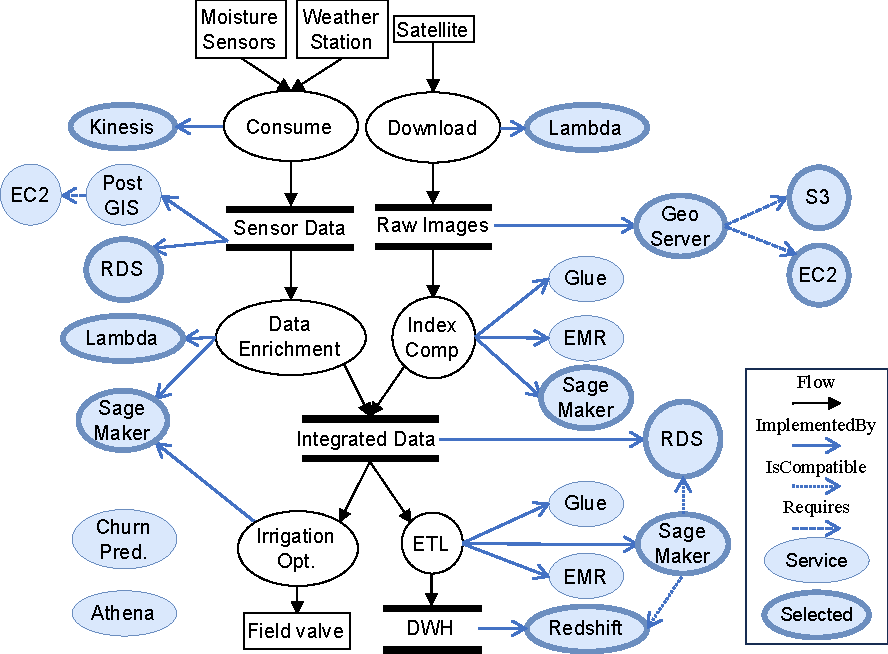
\includegraphics[width=0.75\textwidth]{parts/methods/images/graph.pdf}
    \caption{Matching the DFD (white) and service (blue) graphs; in bold the services selected as the optimal blueprint for the data platform design. \serv{Athena} and \serv{Churn Prediction} are examples of unmatched services that are available in the AWS ecosystem.}
    \label{fig:pdd-match}
\end{figure}

\begin{definition}[Matched graph]
\label{def:pdd-match}
Given a DFD $G^D = (N^D, A^D, P^D, L^D)$ and a service graph $G^S = (N^S, A^S, P^S, L^S)$, a matched graph $G^M = (N^D \cup N^S, A^D \cup A^S \cup A, P^D \cup P^S, L^D \cup L^S \cup \{\lbl{ImplementedBy}\})$ is a directed property graph obtained as the union of $G^S$ and $G^D$. $A$ is an additional set of arcs, one for every match between nodes in $N^S$ and $N^D$. Arcs in $A$ are labeled as \lbl{ImplementedBy} and can have an optional property \prop{Mandatory}{True} to specify that such implementation must be selected in the final blueprint.
\end{definition}

The result of a match is a graph that is composed of the union of the nodes, and the union of the arcs plus additional arcs that represent candidate implementations for the DFD processes/repositories. The label \lbl{ImplementedBy} represents whether a DFD process or repository can be implemented by a specific service. If no match is found for a DFD node, we alert the designer in order to verify that the DFD has been properly designed and/or enriched with the service tags.

\begin{example}[Matched graph]
\Cref{fig:pdd-match} depicts an excerpt of the matched graphs for the DFD from \Cref{fig:pdd-dfd}; for the sake of clarity, not all the arcs have been presented. Nodes from the DFD have a white background, while services are represented in blue. Solid arrows represent arcs labeled as \lbl{ImplementedBy} (e.g., \dfd{Sensor Data} can be implemented by either \serv{PostGIS} or \serv{RDS}). Dotted arrows represent arcs labeled as \lbl{IsCompatible} (e.g., \serv{SageMaker} reads from and writes to \serv{Redshift}). Dashed arrows represent arcs labeled as \lbl{Require} (e.g., \serv{GeoServer} requires \serv{EC2} since it is deployed on it). Of course, it is unlikely that all services of the cloud ecosystem will be matched; \serv{Athena} and \serv{Churn Prediction} are examples of unmatched services.
\end{example}

\subsubsection{Augmenting and Pruning the Matched Graph}

Designing a platform is not just a technical task but encompasses various organizational, business, and political aspects that must be carefully considered. The successful creation of a platform requires the expertise and experience of designers to manipulate the matched graph and aid in the subsequent optimization. This ensures that the platform is not only technically sound but also aligns with broader strategic goals and user needs.

In our approach, designers have several tools at their disposal to influence and refine the design process:
\begin{itemize}
    \item Force the selection of specific services: designers can mandate the inclusion of certain services due to various factors such as client requirements, industry standards, or established design practices. This is accomplished by adding the property \prop{Mandatory}{True} to \lbl{ImplementedBy} arcs in the matched graph. By doing so, designers ensure that essential services are incorporated into the platform.
    \item Prefer certain services over others: in many cases, some services are more desirable than others due to their superior efficiency, reliability, or user familiarity. Designers can indicate these preferences by adding the property \prop{Preferred}{True} to the nodes labeled as \lbl{Service} in the matched graph. This preference can optimize the platform's blueprint and user experience by prioritizing the most advantageous services.
    \item Refine the match: designers can fine-tune the matched graph by preliminarily removing services that do not meet specific criteria or adding services that were initially unmatched. For example, they might exclude services that do not support required programming languages for legacy software or add missing matches due to incomplete tagging. This refinement ensures the platform is both relevant and comprehensive, accommodating all necessary components and integrations.
\end{itemize}

\begin{example}[Mandatory and preferred services]
With reference to \Cref{fig:pdd-match}, imagining that our methodology is used to lift-and-shift an on-premises solution that already used \serv{GeoServer} to AWS, \serv{GeoServer} could be tagged with the property $\prop{Mandatory}{True}$ since clients already have experience with it (and not with alternative engines such as \serv{GoogleEarth}). Also, since \serv{S3} is cheaper than other storage services (such as \serv{EBS} and \serv{EFS}), \serv{S3} could be tagged with the property $\prop{Preferred}{True}$.
\end{example}

After manual adjustments, an automated pruning process removes sub-graphs that are not reachable from the DFD. These sub-graphs represent services that are neither candidate implementations nor accessible from candidate implementations.

\begin{example}[Pruning the matched graph]
In \Cref{fig:pdd-match}, \serv{Churn Prediction} and \serv{Athena} are discarded before the optimization since they are not reachable from any DFD entity (i.e., they are neither candidate implementations nor required by other services).
\end{example}

Finally, this step supports the recognition, matching, and refinement of design patterns, as discussed in \Cref{sec:pdd-patterns}. Design patterns ensure that the data platforms adhere to best practices and maintain a high standard of quality and maintainability.

\subsubsection{Optimizing the Blueprint}
\label{ssec:pdd-opt}

The optimization of the services comprising a data platform can take various forms, depending on the numerous influencing factors and the diverse objectives of clients, such as cost reduction, simplified management, or enhanced extensibility. In this chapter, we use the minimization of the number of services as an objective function since this indicator correlates with both cost minimization and management simplicity. It will be seen later that other desirable properties of the chosen solution (e.g., adherence to business practices and compatibility with other systems already present in the company) can be easily satisfied through the preferences indicated by users.

However, such optimization is not trivial. For instance, some DFD entities can be implemented atop alternative services (e.g., a data lake that is implemented either on \serv{S3} or \serv{HDFS}), and some services are meaningful only if they cover at least two DFD entities (e.g., we use a \serv{Lakehouse} to replace both a data lake and a data warehouse). The selection must be compliant with the following conditions.
\begin{itemize}
    \item \textit{Coverage}: all processes and repositories in the DFD must be covered.
    \item \textit{Dependency}: if a service is selected, all its required services must be (recursively) selected too (e.g., \serv{Geoserver} is deployed on \serv{EC2}).
    \item \textit{Compatibility}: a service can be selected only if it is compatible with the services selected for the previous (if existing) and following (if existing) nodes in the DFD.
    \item \textit{Preference}: services marked as preferred should have more chances to be selected (for instance, preferences can be expressed for services entailing lower costs or higher performance).
    \item \textit{Mandatory}: service implementations marked as mandatory must be selected for the blueprint (e.g., a certain repository must be implemented by a document-based service).
    \item \textit{Affinity}: if a service is selected, services with high affinity should be selected too.
\end{itemize}

\begin{figure}[htbp]
{\footnotesize
\begin{align}
&min \sum_i w_i s_i \textup{ such that }\\
&s_i \in \{0,1\} \textup{ for all } n_i \in N, label(n_i) = \lbl{Service}\\
&s_{ij} \in \{0,1\} \textup{ for all } a_{ij} \in A, label(a_{ij})= \lbl{ImplementedBy}\\
&s_j \geq s_{ij} \textup{ for all } s_{ij}\\
&\sum_{a_{ij} \in A, label(a_{ij})=\lbl{ImplementedBy}} s_{ij}=1  \textup{ for all } n_i \in N, label(n_i) \in \{\lbl{Process}, \lbl{Repository}\}\\
&s_j\geq s_i  \textup{ for all } a_{ij} \in A, label(a_{ij})= \lbl{Requires} \\
&s_{ij}+s_{kh} \leq 1  \textup{ for all } a_{ik} \in A, a_{jh} \notin A, label(a_{ik})=\lbl{Flow}, label(a_{jh})=\lbl{IsCompatible}\\
&s_{ij} = 1 \textup{ for all } a_{ij} \in A, \prop{Mandatory}{True} \in props(a_{ij})\\
&s_{ij} \cdot s_{kh} \geq s_{h} \textup{ for all } a_{ik}, a_{jh} \in A, label(a_{ik})=\lbl{Flow}, label(a_{jh})=\lbl{IsAkin}
\end{align}
}
\caption{Selecting the optimal services considering coverage (5), dependency (6), compatibility (7), and mandatory (8), and affinity (9) constraints.}
\label{fig:pdd-form}
\end{figure}

More formally, given a matched graph $G^M=(N, A, P, L)$, the selection of the optimal blueprint can be modeled as a linear programming problem inspired by the standard \emph{facility location problem}. In a basic formulation, the facility location problem consists of a set of potential facility sites where a facility can be opened, and a set of demand points that must be serviced. The goal is to pick a subset of facilities to open while minimizing the sum of distances from each demand point to its nearest facility plus the sum of opening costs of the facilities. In our case, services are mapped to the potential locations while DFD nodes are mapped to the demand points. The formulation in \Cref{fig:pdd-form} reads as follows.
\begin{itemize}
    \item[(1)] The optimization function minimizes the weighted sum of the selected services. Weights $w_i$ specify preferences for services $s_i$, we set
    \[
    w_i=\begin{cases}
    0.5 & \textup{if } \prop{Preferred}{True} \in props(n_i)\\
    1.0 & \textup{otherwise}
    \end{cases}
    \]
    In case multiple optimal solutions exist, we return all of them to the designers so that they can compare them and select the one they find the most appropriate since there is no solution dominating the others. When no solution is feasible (e.g., due to a lack of matches or incompatibility of mandatory services) the system alerts the designers since a refinement of the DFD could be necessary.
    \item[(2)] $s_i$ are binary variables modeling services. $s_i=1$ if the service is selected, $0$ otherwise.
    \item[(3)] $s_{ij}$ are binary variables modeling the services implementing DFD processes and repositories. $s_{ij}=1$ if $n_i \in N$ s.t. $label(n_i) \in \{\lbl{Repository}, \lbl{Process}\}$ is implemented by $n_j \in N$ s.t. $label(n_j) = \lbl{Service}$.
    \item[(4)] Binding variables $s_j$ and $s_{ij}$: service $s_j$ is selected if it implements ($s_{ij}=1$) a DFD node $n_i \in N$ s.t. $label(n_i) \in \{\lbl{Repository}, \lbl{Process}\}$.
    \item[(5)] \emph{Coverage} constraints: every repository and process must be implemented by exactly one service.
    \item[(6)] \emph{Dependency} constraints: if a service is selected, all the services it depends on must be selected.
    \item[(7)] \emph{Compatibility} constraints: if two services are incompatible, they cannot be selected to implement two consecutive processes/repositories linked through a data flow in the DFD.
    \item[(8)] \emph{Mandatory} constraints: if an implementation is mandatory and tagged with the property \prop{Mandatory}{True}, $s_{ij}$ is set to 1.
    \item[(9)] \emph{Affinity} constraints: if the service $s_h$ is selected and has affinity with another service $s_j$, then $s_j$ is selected too.
\end{itemize}

\begin{example}[Optimization]
\label{ex:pdd-optimization}
Given the matched graph from \Cref{fig:pdd-match}, the \textit{optimal} blueprint of the data platform is represented by the services highlighted in bold (with a cost of 7.5), namely \serv{Kinesis}, \serv{Lambda}, \serv{RDS}, \serv{EC2}, \serv{SageMaker}, \serv{GeoServer}, \serv{S3} (tagged as preferred), and \serv{Redshift}. \serv{GeoServer} has been selected since it is the only available implementation for \dfd{Raw Images}, \serv{EC2} and \serv{S3} have been selected since they are required by \serv{GeoServer}. \serv{SageMaker} has been selected and preferred to \serv{EMR} and \serv{Glue} since three DFD processes can be implemented on it.
\end{example}

\subsection{Design Patterns}
\label{sec:pdd-patterns}

Clients' data pipelines could present \textit{design patterns} (i.e., solutions to common problems in software and architecture design) that require certain constraints to be satisfied on the overall data pipeline (and not only on single nodes in the DFD and their properties). Design patterns are important since they impact the services that are matched and selected for the optimal blueprint.

\subsubsection{Defining Design Patterns}

Design patterns are retrieved from the DFD graph.
\begin{definition}[Architectural Design Pattern]
Given a DFD graph $G^D$, a design pattern $p$ is a subgraph $\bar{G} \in G^D$ in which $cond_p(\bar{G})$ holds. $cond_p(\bar{G})$ is specific to each design pattern and can be expressed in terms of graph queries on the DFD graph.
\end{definition}

Since our definition of design pattern is ``generic'', design patterns could impact our approach in different ways. The simple recognition of design patterns could already be informative for the designer of the data platform (the recognition of the pattern itself could help to refine the design of the platform). Additionally, patterns could alter the matched graph (by matching additional services) and the optimization procedure (by preferring some services to others). We show the impact of design patterns with reference to the \textit{Lakehouse} and \textit{Lambda Architecture} (although other patterns exist, such as the kappa architecture and the 2- or 3-layered architecture for data warehousing).

\paragraph{Lakehouse.} Lakehouse (\Cref{fig:pdd-matchlake}) is a data management paradigm that combines the capabilities of data lakes and data warehouses, enabling business intelligence and machine learning on the same data. A Lakehouse can be applied if, within the same data pipeline, there is a sequence of ETL steps that moves data from a data lake to a data warehouse, optionally passing through relational databases. Lakehouse encourages the adoption of a medallion architecture (a data design pattern)\footnote{\url{https://www.databricks.com/glossary/medallion-architecture}} where raw data is initially stored in a data lake (bronze layer), refined data are stored in a relational engine (silver layer), and data cubes are stored in a multidimensional engine (gold layer). However, to avoid the additional usage of a relational engine (which would bring higher costs and effort into keeping the 3 layers aligned), ETL could skip the intermediate storage and upload data directly into the data warehouse for simpler architectures.

Formally, a Lakehouse is a graph $\bar{G}$ with a set of nodes $\bar{N}=\{n_i, ..., n_k, ..., n_j\}$ such that $cond_{Lakehouse}(\bar{G})$ is defined as
\begin{align*}
&\exists p_{ij} ~ s.t. ~ label(n_i) = Repository \wedge \prop{Functionality}{Landing} \in prop(n_i) \wedge\\
&\qquad\qquad            label(n_j) = Repository \wedge \prop{Data Model}{Multidimensional} \in prop(n_j)
\end{align*}
and (optionally) $n_k \in p_{ij}.nodes ~ s.t. ~ \prop{Data Model}{Structured} \in prop(n_k)$. Intuitively, $n_i$ is the data lake, $n_j$ the data warehouse, and $n_k$ the optional intermediate relational storage.

\paragraph{Lambda Architecture.} Lambda architecture (\Cref{fig:pdd-lambda}) is a data-processing architecture designed to handle massive quantities of data by taking advantage of both batch and stream processing. It uses batch processing to provide comprehensive and accurate views of batch data, while simultaneously using real-time stream processing to provide views of online data. Formally, a Lambda architecture is a graph $\bar{G}$ with a set of nodes $\bar{N}=\{n_i, n_j, n_k, n_l\}$ such that $cond_{Lambda}(\bar{G})$ is defined as the conjunction of the following conditions
\begin{align*}
&\exists p_{ij} ~ s.t. ~ label(n_i) = Process \wedge \prop{Collection}{Push} \in prop(n_i) \wedge\\
&\qquad\qquad label(n_j) = Process \wedge \prop{Computing}{Streaming} \in prop(n_j),\\
&\exists p_{ik} ~ s.t. ~ label(n_k) = Repository \wedge \prop{Volume}{Big} \in prop(n_k),\\
&\exists p_{kl} ~ s.t. ~ label(n_l) = Process \wedge \prop{Computing}{Batch} \in prop(n_l)
\end{align*}

\subsubsection{Exploiting the Matched Graph}

Design patterns can be highlighted to designers for further evaluation or match additional services. For instance, new matches are added when design patterns can be directly implemented by services from the service graph. This is the case for Lakehouse, where a single service fulfills the requirements of an entire pattern.

\begin{figure}[htbp]
\centering
%[FIGURE: matching del pattern Lakehouse -- in grigio i processi non rilevanti, in rosso la property che impedisce il match tra Raw Images e Lakehouse]
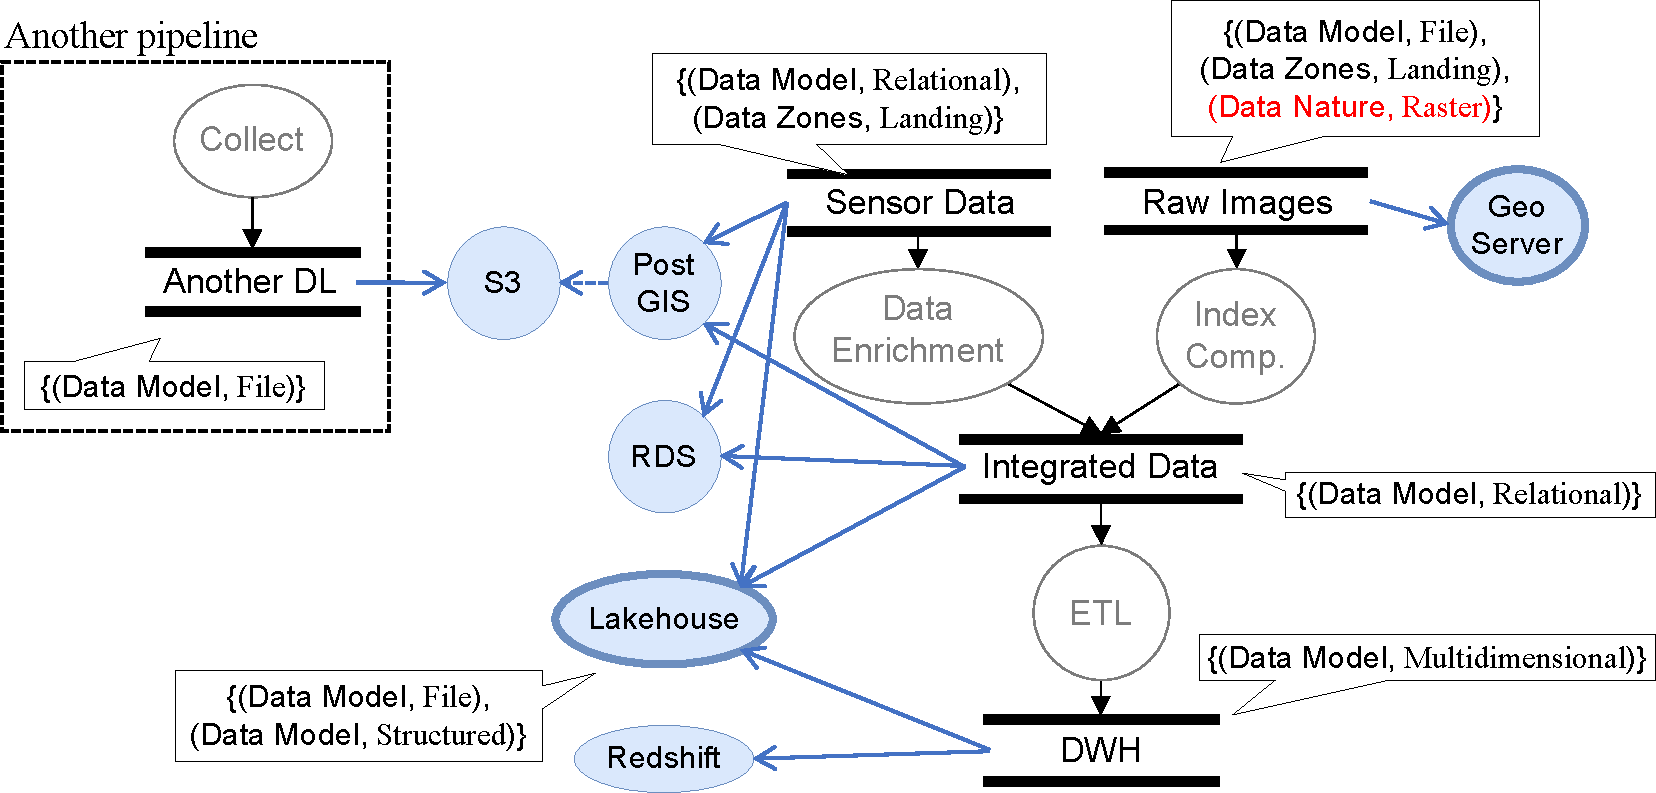
\includegraphics[width=0.8\textwidth]{parts/methods/images/matchingdl.pdf}
\caption{Matching the Lakehouse pattern; in gray the processes that are not relevant for matching the Lakehouse pattern and in red the property preventing the match between \dfd{Raw Images} and \serv{Lakehouse}.}
\label{fig:pdd-matchlake}
\end{figure}

\paragraph{Lakehouse.}

Databricks' \serv{Lakehouse} is a multi-platform service that implements the Lakehouse pattern. Given a DFD graph including one (or more) Lakehouse pattern $\bar{G}$ with nodes $\bar{N}$ and a service graph including the node $n_s=\serv{Lakehouse}$, the matched graph $G^M$ is augmented with new arcs $(N^M, A^M \cup A, P^M, L^M)$ where $A = \{a_{is} ~s.t.~ match(n_i, n_s) = true, n_i \in \bar{N}\}$ is an additional set of arcs, one for every (property) match between nodes in $\bar{N}$ and $n_s$. Arcs in $A$ are labeled as \lbl{ImplementedBy}.

In other words, the Lakehouse is a potential implementation for the DFD repositories in the path connecting a data lake to a data warehouse.

\begin{example}[Design pattern match]
\Cref{fig:pdd-matchlake} depicts two examples of matching the service \serv{Lakehouse} (processes are grayed out since they are not relevant for matching the Lakehouse pattern). \serv{Lakehouse} does not match \dfd{Another DL} since the latter belongs to a pipeline without a data warehouse. Conversely, \serv{Lakehouse} matches \dfd{Sensor Data}, \dfd{Integrated Data}, and \dfd{DWH} since in the DFD graph exists a path connecting a landing area (\dfd{Sensor Data}) to a data warehouse (\dfd{DWH}) and optionally passing through a relational repository (\dfd{Integrated Data}). In other words, this data pipeline is organized according to the medallion architecture that can be implemented by \serv{Lakehouse}. Additionally, \serv{Lakehouse} does not match \dfd{Raw Images} since it has the property \prop{Data Nature}{Raster} and \serv{Lakehouse} cannot directly manage spatial data/queries (more formally $match(\dfd{Raw Images}, \serv{Lakehouse}) = false$). Noticeably, if \serv{Lakehouse} is matched and later selected in place of \serv{RDS} and \serv{Redshift}, the cost of the solution in \Cref{ex:pdd-optimization} and \Cref{fig:pdd-match} decreases from 7.5 to 6.5.
\end{example}

\paragraph{Lambda Architecture.}
The lambda architecture does not require any augmentation since the composition of the services necessary for its implementation is already matched through the properties of single nodes. However, as we will see immediately below, its exploitation is accomplished by a modified formulation of the optimization problem.

\begin{figure}[htbp]
\centering
%[FIGURE: pattern Lambda architecture -- sorgente streaming/processing streaming, big data storage, big data batch engine]
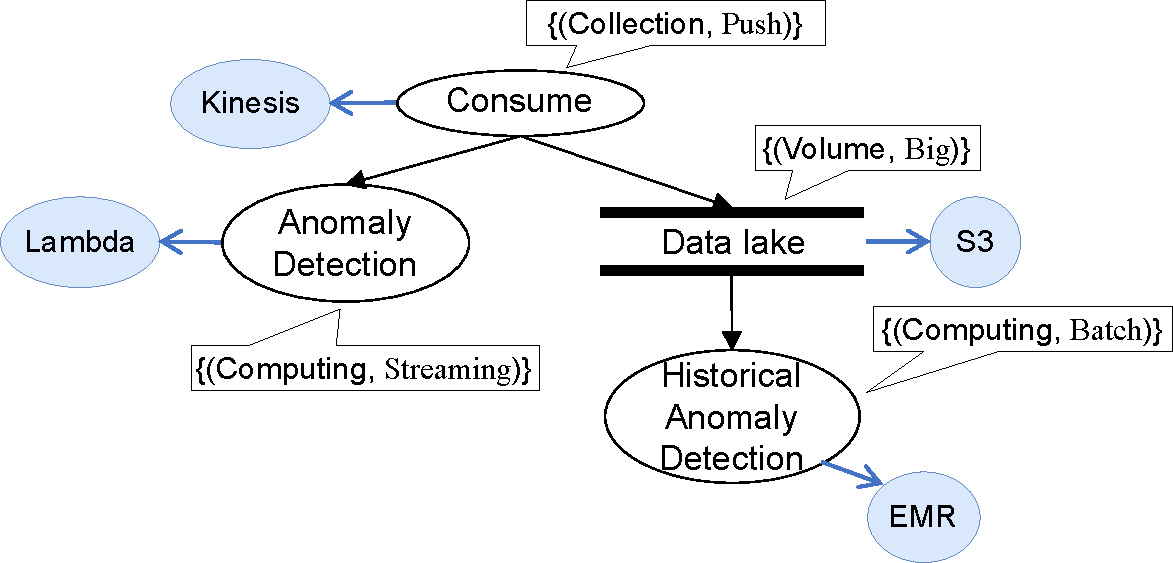
\includegraphics[width=0.7\textwidth]{parts/methods/images/lambda.pdf}
\caption{Lambda pattern.}
\label{fig:pdd-lambda}
\end{figure}

\subsubsection{Refining the Optimization}

To implement the design patterns, additional constraints could be plugged into the optimization or the weights of some services could be adjusted to prefer the adoption of some services to others.

\paragraph{Lakehouse.}

The adoption of the Lakehouse pattern $\bar{G}$ with nodes $\bar{N}=\{n_i,...,n_k,...,n_j\}$ (with $n_i$ representing a data lake, $n_j$ representing a data warehouse, and $n_k$ is an optional structured repository in between the data lake and the data warehouse) requires that, if \serv{Lakehouse} service $n_s$ is picked (i.e., $s_s=1$), such service must cover the data lake and the data warehouse as well as the optional intermediate structured repositories (there is no point in having a partial implementation of a \serv{Lakehouse}).
{\footnotesize
\begin{align*}
s_{is}\cdot ... \cdot s_{ks} \cdot ... \cdot s_{js} > s_s   \textup{ for all }& a_{is}, a_{ks}, a_{js} \in A,\\
& label(a_{is})=label(a_{ks})=label(a_{js})=\lbl{ImplementedBy}
\end{align*}
}

\paragraph{Lambda Architecture.}

The adoption of the Lambda architecture $\bar{G}$ with nodes $\bar{N}=\{n_i,n_j,n_k,n_l\}$ (with $n_i$ representing a streaming source, $n_j$ a streaming processing, $n_k$ a big data storage, and $n_l$ a big data engine) does not require additional constraints but pushes towards the adoption of some services. For instance, the AWS documentation usually leverages \serv{S3} as a big data storage, \serv{EMR} as a big data engine, \serv{Kinesis} as a streaming source, and \serv{Lambda} as streaming processing (although different services could be used, such as queuing services in place of \serv{Kinesis}). Since these services are \textit{recommended} by AWS to create a Lambda Architecture, their properties are extended with the additional property $\prop{Preferred}{True}$.
\begin{align*}
&props(\serv{S3}) = \{\prop{Preferred}{True}\} \cup props(\serv{S3})\\
&props(\serv{EMR}) = \{\prop{Preferred}{True}\} \cup props(\serv{EMR})\\
&props(\serv{Kinesis}) = \{\prop{Preferred}{True}\} \cup props(\serv{Kinesis})\\
&props(\serv{Lambda}) = \prop{Preferred}{True} \cup props(\serv{Lambda})
\end{align*}
Given the optimization problem formulated in \Cref{ssec:pdd-opt}, from Line (1) it follows that $w_i = 0.5 \textup{ if } s_i \in \{\serv{S3}, \serv{EMR}, \serv{Kinesis}, \serv{Lambda}\}$ since $w_i$ is set to 0.5 if $\prop{Preferred}{True} \in props(s_i)$. In other words, weights are decreased to 0.5 to bias the optimization towards the selection of the four services.

\subsection{Evaluation}
\label{sec:pdd-eval}

We implemented our approach (available at \url{https://github.com/big-unibo/DataPlatformDesign}) using GraphDB (to store the taxonomy of tags, the service graph, and the DFD diagrams) and Python, where we leverage the CPlex library to solve the optimization problem.

\subsubsection{Validation with Real Use Cases}
\label{sec:pdd-val}

To assess the approach, we applied it in two real contexts\footnote{We anonymize the names of the companies due to non-disclosure agreements.}: Company1 (one of the largest Italian consulting firms specialized in data analysis and with strong expertise in the field of data platforms and cloud computing) and Company2 (an international company leading in the production of smart and digitalized sports equipment). In particular, (i) we asked their experts for two use cases of data platforms implemented on different cloud service providers to prove the portability of our approach, (ii) we generated a blueprint for each use case, (iii) we asked the experts to evaluate and compare our blueprints against the ones they implemented.

In this experimental setup, we act as platform designers, whereas experts from the companies act as clients. The collection of the case studies was done by setting up 2 to 3 interviews of a maximum of 1 hour each and according to the methodology from \Cref{sec:pdd-overview}.

\begin{itemize}
    \item Step (1): we created the service graphs for Microsoft Azure and Google Cloud. We adopted the taxonomy of tags summarized in \Cref{tab:pdd-tags}.
    \item Step (2): the first interview was devoted to understanding the proposed data-driven processes: the main steps, subjects, and analysis goals. The output of the interview was the DFD diagram of the processes.
    \item Steps (3) and (4): we enriched the DFD with tags from our taxonomy and matched it with the service graphs.
    \item Step (5): the second interview was devoted to refining the DFD and augmenting the matched graph with the clients. This additional iteration on the DFD is necessary in case of ambiguities in the tagging.
    \item Step (6): we generated the blueprint and used the final interview to discuss the solution with the clients.
\end{itemize}

\begin{figure}[htbp]
    \centering
    %[FIGURE: matched graph e servizi selezionati per il caso studio 1 (KPI factory)]
    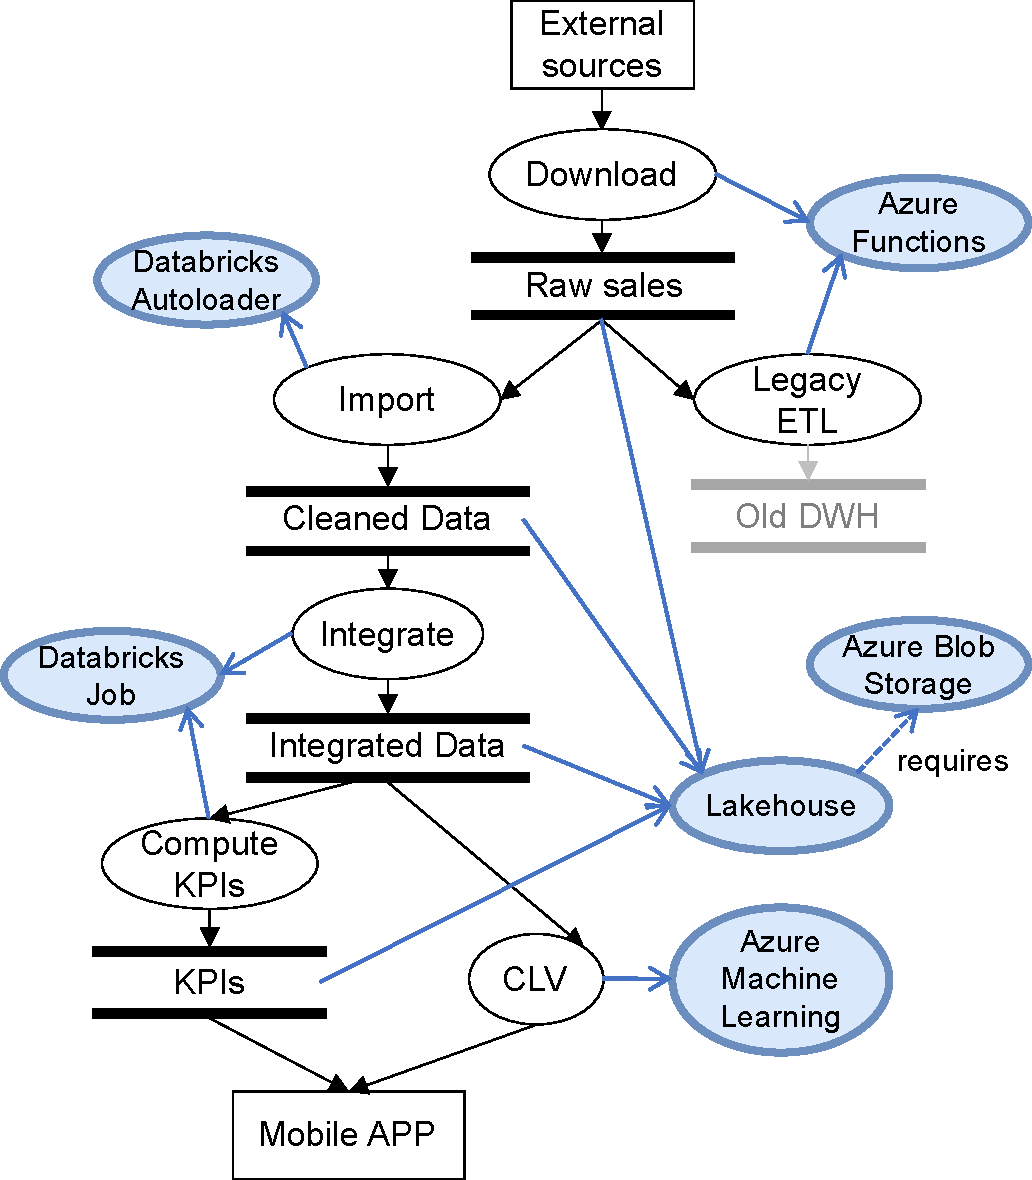
\includegraphics[width=0.55\textwidth]{parts/methods/images/ico.pdf}
    \caption{Matched graph and selected services for case study \#1.}
    \label{fig:pdd-cs1}
\end{figure}

Here follows a description of the Case Studies (CS). Their DFDs along with their blueprints are represented in \Cref{fig:pdd-cs1,fig:pdd-cs2}.

\begin{example}[CS\#1: creating a KPI factory]
Starting from an on-premises data warehouse that has reached a performance plateau, a sales company aims to create a KPI factory: a centralized system where all KPIs are incrementally computed. The data warehouse only supports KPI calculations four times a day, but the company needs more frequent updates. The KPI calculation starts with sales data being drawn from external sources every hour via HTTP API. This data is then stored in its original format, cleaned, integrated, and made usable on a multidimensional engine. It is crucial to store the data at each processing step to facilitate different levels of analysis. For instance, the integrated data is utilized for machine learning models to estimate customer lifetime value. The calculated KPIs are sent to applications managed by client advisors for client-telling actions and are accessible via JDBC connectors. Additionally, the (old) data warehouse must continue to be updated with new data through its legacy ETL procedure. Since the on-premises data warehouse is out of the scope of the platform, we grayed it out in \Cref{fig:pdd-cs1}.
\end{example}

\begin{figure}[htbp]
    \centering
    %[FIGURE: matched graph e servizi selezionati per il caso studio 2 (customer lifetime value forecasting)]
    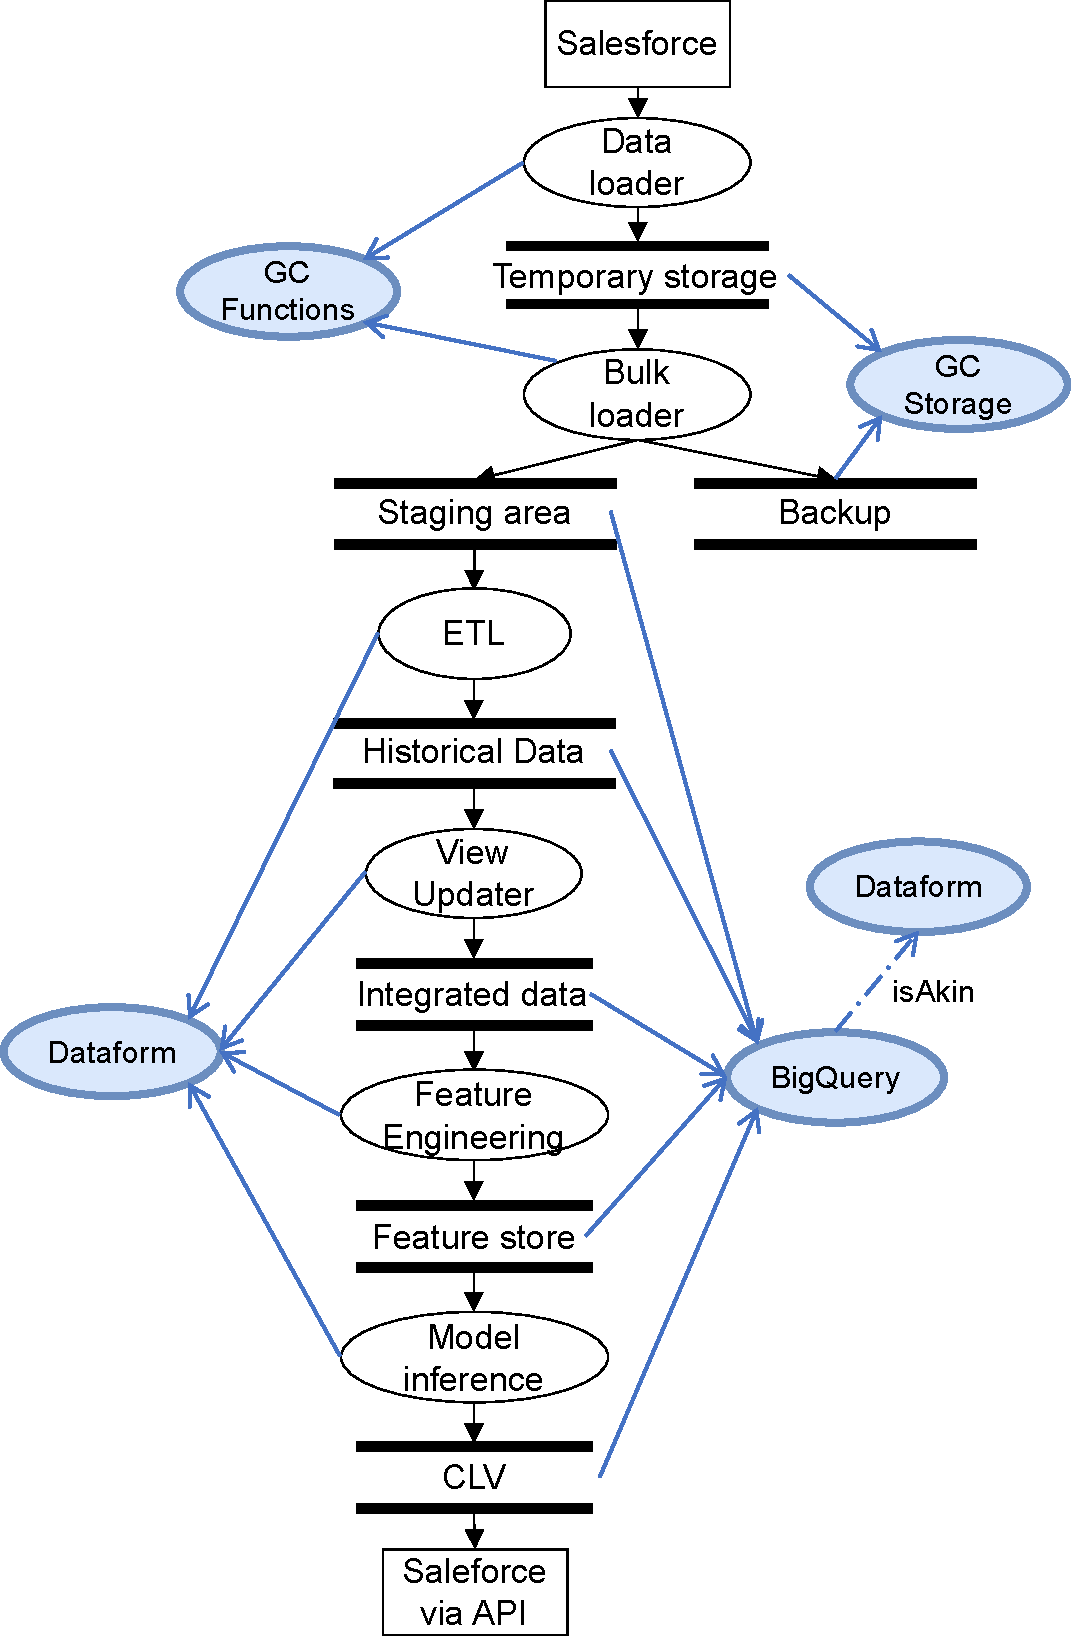
\includegraphics[width=0.5\textwidth]{parts/methods/images/technogym.pdf}
    \caption{Matched graph and selected services for case study \#2.}
    \label{fig:pdd-cs2}
\end{figure}

\begin{example}[CS\#2: forecasting customer lifetime value]
From a Salesforce CRM ecosystem, users' data is extracted every thirty minutes via API calls leveraging a change-data-capture mechanism and is stored in .csv files. Daily, such .csv files are then pushed into two buckets: the first acts as an ingestion backup storage while the other serves as a staging area. From the latter on, data flows through an ETL procedure that updates both the historical trend and the real-time view of each user. The output of the ETL procedure is transformed through feature engineering and fed to a machine learning model predicting the customer lifetime value. Finally, inferred data is filtered and copied into the Salesforce CRM via a custom application.
\end{example}

All in all, we draw the following conclusions.
\begin{itemize}
    \item \textbf{Blueprints effectiveness.} The blueprints returned by our system are compatible and overlap with the ones actually adopted by the companies. In CS\#1, our solution matches the company's solution with 6 services out of 7. The only difference is \serv{Azure Machine Learning}. The company preferred to keep the machine learning activity within the Databricks ecosystem rather than in Azure. This could be fixed by imposing a mandatory service to fulfill the \serv{CLV} process. Similarly, in CS\#2 we matched 4 services out of 5 since we adopted \serv{Google Cloud Functions} for the \dfd{Data Loader} process but the company preferred to use \serv{GSUtils} within the \serv{Google Cloud CLI} (command line interface). \serv{BigQuery} is akin to \serv{Dataform} since \serv{Dataform} operationalizes scalable data transformations pipelines in \serv{BigQuery} using SQL \cite{dataform}.

\item \textbf{Methodology effectiveness.} The requirement analysis was smooth and the staff from the two companies had no problem describing the data-processes and answering questions needed for tagging. The case study from Company1 required a refinement of the DFD since it involved several organizational constraints. For instance, the \dfd{Raw Sales} repository is handled by a different department than the one handling the repositories \dfd{Cleaned Data}, \dfd{Integrated Data}, and \dfd{KPIs}. This organizational constraint impacts the blueprint. On the one hand, if the two departments were willing to share the same technological solution, then all repositories could be implemented by \sf{Lakehouse} even though their management would be separated (as in \Cref{fig:pdd-cs1}). On the other hand, if \dfd{Raw Sales} should be detached from the following part of the pipeline, then it would implemented using \serv{Azure Blob Storage} rather than \serv{Lakehouse} (being a data lake that is not eventually connected to a data warehouse, we correctly discard \serv{Lakehouse} as a possible implementation).
\end{itemize}
Both companies acknowledged that selecting services for a project is highly complex and that staying up to date about service provider offerings requires considerable time and effort. Overall the experts were enthusiastic about the approach and highlighted the following strengths: (i) it can support and train young designers for the creation of blueprints, (ii) it can remove bias in the selection of services (e.g., consultants mainly working with a hyperscaler could tend to prefer services that hyperscaler), and (iii) it is an objective approach to compare different blueprints. Although the blueprints are not perfectly overlapping, experts claim that our blueprints are correct from a technical and technological point of view. However, what could be improved in our approach is the integration of more organizational, political, or even familiarity constraints that could bias the service selection. Our approach partially addresses these issues during the augmentation of the matched graph (e.g., with properties \lbl{IsAkin}, \prop{Mandatory}{True}, and \prop{Preferred}{True}) but could benefit by allowing further expressiveness.

\subsubsection{Efficiency}

We test how our approach scales up to bigger cloud ecosystems and data pipelines, both translating into bigger service and DFD graphs with more nodes and relationships.

To do so, we implement additional synthetic pipelines (i.e., DFDs with increasing nodes $|N^D|$) that share the service ecosystem and the taxonomy of tags. DFDs are created using a tree structure that is randomly expanded until a given number of nodes is reached. The shared service ecosystem contains 200 services with a compatibility rate of 95\% (that is, each service is compatible with 95\% of the others). Each service is enriched with a pair of tags randomly extracted from the shared taxonomy (using a uniform distribution). Finally, each node in the DFD is enriched with a pair of tags selected from the set of tag pairs previously assigned to the services within the service ecosystem. This ensures that every node in the DFD is implemented by at least one service.

To assess the scalability of the approach, the synthetic pipelines differ by a factor of 5x in terms of the number of nodes composing each DFD, starting with DFDs of 10 nodes (as for the real pipelines described in \Cref{sec:pdd-val}) up to 250 nodes.\footnote{We use DFDs of 250 nodes to stress our system although we believe that they are hardly manageable in real applications.} For each number of nodes $N^D \in [10, 50, 250]$ we randomly generate 10 DFD graphs and \Cref{tab:pdd-scalability} and \Cref{fig:pdd-scalability} summarize the average results. Overall, our approach scales well to scenarios involving 200 services and 250 data processes/repositories in the DFD, with a computational time of less than 10 seconds. The time necessary for augmentation and pruning is negligible, whereas matching dominates the total time (93\% for 250 nodes). Matching could be improved by further optimizing GraphDB since the match is automatically solved by the reasoner.

\begin{table}[htbp]
    \centering
    \caption{Breakdown of performance (in seconds) by increasing the nodes of the DFD.}
    \label{tab:pdd-scalability}
    \begin{tabular}{c|ccc|c}
    \toprule
    $|N^D|$ & Match & Augment & Select & Total \\
    \midrule
    10 & 0.22  & $4 \cdot 10^{-5}$ & 0.17 & 0.38 \\
    50 & 0.87  & $4 \cdot 10^{-5}$ & 0.26 & 1.13 \\
    250 & 7.23 & $5 \cdot 10^{-5}$ & 0.53 & 7.76 \\
    \bottomrule
    \end{tabular}
\end{table}

\begin{figure}[htbp]
    \centering
    %[FIGURE: stacked bar chart delle performance (match/augment/select) al crescere della dimensione del DFD]
    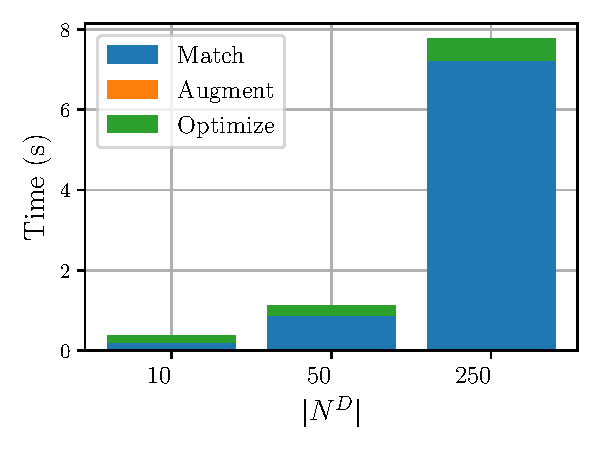
\includegraphics[width=0.7\textwidth]{parts/methods/images/stacked_bar_chart.pdf}
    \caption{Performance by increasing the size of the DFD.}
    \label{fig:pdd-scalability}
\end{figure}

\subsection{Related Work}
\label{sec:pdd-related}

Understanding which ``building blocks'' should be part of a data platform is nontrivial. Several functional architectures (system representations that focus on its functions and their interactions) have been proposed. NIST designed the Big Data Reference Architecture \cite{chang2019nist} which comprised vendor-, technology- and infrastructure-independent logical functional components that are necessary for managing and processing big data (data provider, data consumer, system orchestrator, big data application provider, and big data framework provider). Lambda \cite{DBLP:conf/bigdataconf/KiranMMDB15} is an architecture designed to handle massive quantities of data by taking advantage of both batch and stream-processing methods. Kappa \cite{kreps2014questioning} overcomes some limitations (e.g., ``redundant'' batch and streaming implementations) of Lambda by using a pure streaming approach with a single code base. While these architectures define functional components necessary for (big) data platforms, they are abstract and do not address the problem of selecting the optimal services necessary for designing, implementing, and deploying working data platforms.

Cloud service providers such as Amazon \cite{aws}, Google \cite{gcp}, and Microsoft \cite{azure} provide ecosystems of independent and interoperable services. While ecosystems enable easy deployment of data pipelines, choosing the \textit{optimal} services is hard: (i) each provider offers different services, (ii) a shared categorization and organization of services is missing, and (iii) it is hard for the users to understand which services are needed based on their data-driven processes \cite{DBLP:journals/jnca/SunDHHC14}. Some multi-objective optimization techniques have been proposed, where users express requirements and preferences (e.g., minimal QoS) about single services \cite{DBLP:conf/ncca/CavalcanteLBCDP11,DBLP:journals/cluster/NejatMVB22,DBLP:journals/jss/LuY18}, cloud deployment models (public and private) \cite{DBLP:journals/tcc/Garg22}, and service providers \cite{DBLP:journals/eswa/KarKPK23,DBLP:journals/cluster/TomarKG23}. Finally, domain languages and ontologies have been introduced (e.g., \cite{DBLP:conf/webi/NouraG19}) to enable some service composition (e.g., \cite{DBLP:journals/jsan/MahfoudhCS21}).

With respect to these works, the novelties of our approach are (i) the introduction of a methodology to enable data platform design, (ii) a computer-aided approach to support designers in their choices, and (iii) process-driven optimization to select the optimal blueprint out of many data flows, even from multiple stakeholders.

\subsection{Conclusion and Future Directions}
\label{sec:pdd-conclusion}

The design of data platforms is a nontrivial task. {\color{red}This chapter} introduced a methodology to aid designers in selecting the optimal services (out of a service ecosystem) supporting data-driven processes from multiple stakeholders (e.g., partners in a research project), and addressed such selection as a facility location optimization problem. Our approach can match and select single services as well as design patterns (e.g., Lakehouse to replace both data lakes and warehouses), it supports additional constraints (e.g., mandatory and affinity), and the produced blueprints have been successfully compared with the ones recommended by expert designers.

We believe that the expressiveness of the approach can still be improved as follows. \textit{Expressiveness}: introduce more advanced constraints to support organizational and political factors in the design of the blueprints. \textit{Resource provisioning}: additionally to selecting the services, a complete approach should also consider how many instances of a service are required (to do so, a cost model should be studied). \textit{Metadata integration}: while catalog and meta-data management services do not directly introduce functionalities for data transformation and exploitation, the design should also recommend services helping in the management of the platform itself \cite{francia2021moses}.

{\color{red}
The metadata-integration direction identified above is taken up directly in the following chapter, which investigates how Large Language Models can support users in querying the metadata of a data-intensive system -- in that case, a data warehouse -- without requiring expertise in its underlying schema, continuing this thesis's preliminary exploration of the mechanisms required for Digital Twins to be understood, and eventually integrated, beyond the boundaries of a single deployment.
}

\section{LLM guided metadata exploration}
\label{sec:llm-guided-metadata-exploration}\
\input{parts/methods/chapters/llm4bi.tex}
%%%%%%%%



%%%%%%%%

\chapter{Applications}
\label{chap:applications}

\section{Data-driven optimization of water consumption in kiwifruit orchards}
\label{sec:smarter}

\section{Anomaly Detection in complex sensor networks}
\label{sec:s2g}


\begin{epilogue}
\chapter{Conclusion and Future Work}
\label{chap:conclusion}

\end{epilogue}

\backmatter

\part*{}

\nocite{*} % comment this to only show the referenced entries from the .bib file
\bibliographystyle{alpha}
\bibliography{phd-thesis}

\end{document}